\documentclass{master-thesis}
\usepackage[
backend=biber,
style=ieee,
language=autobib,
autolang=hyphen
]{biblatex}
\usepackage{amsfonts}

\addbibresource{./03_bibliography/bibliography.bib}

\hyphenation{Put-SIMD-IN-Gate}
\hyphenation{Put-Dummy-SIMD-IN-Gate}
\hyphenation{Put-IN-Gate}
\hyphenation{Put-Dummy-IN-Gate}
\hyphenation{Shan-non}
\hyphenation{De-ter-min-is-tic}

\newacronym{SMPC}{SMPC}{Secure Multi Party Computation, Ασφαλής Υπολογισμός Πολλών Μερών}
\newacronym{2PC}{2PC}{2 Party Computation, μια συγκεκριμένη μορφή SMPC με μόνο δύο συμμετέχοντες}
\newacronym{IoT}{IoT}{Internet of Things, Διαδίκτυο των Πραγμάτων}
\newacronym{TTP}{TTP}{Trusted Third Party, Έμπιστος Τρίτος}
\newacronym{FHE}{FHE}{Fully Homomoprhic Encryption, Πλήρης Ομομορφική Κρυπτογραφία}
\newacronym{HE}{HE}{Homomorphic Enryption, Ομομορφική Κρυπτογραφία}
\newacronym{SHE}{SHE}{Somewhat Homomorphic Encryption, Κάπως Ομομορφική Κρυπτογραφία}
\newacronym{SSS}{SSS}{Shamir Secret Sharing, Διαμοίραση Μυστικών Shamir}
\newacronym{BLAS}{BLAS}{Basic Linear Algebra Subroutines, Βασικές Υπορουτίνες Γραμμικής Άλγεβρας}
\newacronym{RSA}{RSA}{Ronald, Shamir, Ademir, Διάσημο πρωτόκολλο ασυμμετρικής κρυπτογραφίας}
\newacronym{GMW}{GMW}{Goldreich, Micali, Wigderson, Πρωτόκολλο SMPC}
\newacronym{BMR}{BMR}{Ben-Or, Micali, Rogaway, Πρωτόκολλο SMPC}
\newacronym{gcd}{GCD}{Greatest Common Divisor}
\newacronym{lcm}{LCM}{Least Common Multiple}

\begin{document}
    % \improvement{Clarify that in MPC protocols pre-established secure channels are assumed to exist}

\listoftodos

% \nocite{*}

\begin{titlepage}
    \begin{center}
        
\includegraphics[width=0.4\textwidth]{00_preamble/images/upatras.jpg}
        \vspace*{1cm}
        \\ \textsc{Τμήμα Μηχανικών Ηλεκτρονικών Υπολογιστών και Πληροφορικής
        \\Πολυτεχνική Σχολή}
        \vspace{0.3cm}
    \large{
    \textbf{\\ΤΙΤΛΟΣ \\ Μελέτη Πρωτοκόλλων Ασφαλούς Υπολογισμού Πολλών Μερών
    \\ (Study on Secure Multi Party Protocols)}}
        \vspace{0.5cm}
        \\Διπλωματική εργασία \\
        του\\
        \vspace{0.5cm}
        \textbf{ΘΕΟΔΩΡΟΥ ΣΥΜΕΩΝΙΔΗ}\\
        \vspace{1cm}
        
    \end{center}
    \begin{center}
        \begin{tabular}{ c c } 
            \textbf{Επιβλέπων:} & Ιωάννης Σταματίου \\ 
              & Καθηγητής  \\
            \textbf{Συνεπιβλέπων:} & Χρήστος Μακρής  \\ 
              & Αν. Καθηγητής \\ 
            \textbf{Συνεπιβλέπων:} & Αριστείδης Ηλίας \\ 
              & Ε.ΔΙ.Π \\ 

        \end{tabular}
    \end{center}
    \begin{center}
        \vfill
        Πάτρα \today
    \end{center}

\end{titlepage}

\chapter*{Περίληψη}
\addcontentsline{toc}{chapter}{Περίληψη}

\pagestyle{plain}

Στην παρούσα διπλωματική εργασία γίνεται εισαγωγή και μελέτη σε διαφορετικά πρωτόκολλα Υπολογισμού Πολλών Μερών (Secure Multi Party Computation ή SMPC), μερικά από τα οποία στη συνέχεια εφαρμόζονται για τη δημιουργία, της πρώτης στη βιβλιογραφία, BLAS βιβλιοθήκης, για Ασφαλή Υπολογισμό Δύο Μερών, BLAS συναρτήσεων Επιπέδου-1 για πραγματικούς αριθμούς κινητής υποδιαστολής μονής ακρίβειας. Πριν ξεκινήσουμε τη μελέτη αυτή, γίνεται μια εισαγωγή στην κρυπτογραφία και στην αποδείξιμη θεωρητική ασφάλεια παρουσιάζοντας όλο το απαραίτητο θεωρητικό υπόβαθρο, μαθηματικό και αλγοριθμικό, που απαιτείται για τη βαθύτερη κατανόηση του αντικειμένου. Στη μελέτη αυτή εστιάζουμε σε σύγχρονα κρυπτογραφικά εργαλεία που χρησιμοποιούνται σήμερα ως συστατικά στοιχεία για την κατασκευή σύνθετων κρυπτογραφικών σχημάτων, δίνοντας περισσότερη έμφαση σε εργαλεία που χρησιμοποιούνται για την κατασκευή σχημάτων Ασφαλούς Υπολογισμού Πολλών Μερών.

\vspace{0.3cm}

\begin{flushleft}
\huge\textbf{Abstract}
\end{flushleft}

On the current diploma thesis we present an introduction and a study on various Secure Multi Party Computation Protocols (SMPC) where some of them are used next to implement the first SMPC BLAS Level-1 library for single precision real floating point numbers. Before this begin this study, we present an introduction to cryptography and provable theoretical security including all the required mathematical and algorithmic background needed for the deeper understand of the subject. On this study we focus on modern cryptographic tools that are used today as a building part to construct complex cryptographic schemes while giving more focus on the set of these tools that are used mostly in the construction of SMPC schemes.

\chapter*{Ευχαριστίες}
\addcontentsline{toc}{chapter}{Ευχαριστίες}

\pagestyle{plain}

Θα ήθελα να ευχαριστήσω θερμά τους ανθρώπους που συνέβαλαν στην ολοκλήρωση
της παρούσας ιπλωματικής εργασίας αλλά και τους ανθρώπους που στάθηκαν δίπλα μου κατά της περίοδο εκπόνησης της. Θα ήθελα να ευχαριστήσω θερμά τον επιβλέποντα καθηγητή μου, Ιωάννη Σταματίου, καθώς τον συνεπιβλέπον Αριστείδη Ηλία, Ε.ΔΙ.Π. για την πολύτιμη συνεισφορά και βοήθεια τους. Επίσης, θα ήθελα να ευχαριστήσω όλα τα μέλη του εργαστηρίου του κύριου Χρήστου Μακρή, Αναπληρωτή Καθηγητή, στο οποίο βρισκόμουν όλο τον καιρό εκπόνησης αυτής της διπλωματικής εργασίας, για την πολύτιμη βοήθεία τους σε τεχνικά θέματα αλλά και για την καλή τους παρέα. Τα μέλη αυτά είναι ο Αγοράκης Μπομπότας, ο Νικήτας Καλογερόπουλος και ο Παναγιώτης ΚεχαγιάΤέλος. Τέλος, οφείλω ένα μεγάλο ευχαριστώ στην οικογένειά μου, στους φίλους μου και στην κοπέλα μου για την κατανόηση, τη συμπαράσταση και τη στήριξή τους.

\null\vfill
\begin{flushright}
    \textit{Αφιέρωση}
\end{flushright}

\tableofcontents

\listoffigures

\listoftables

\chapter*{List of Acronyms}
\addcontentsline{toc}{chapter}{Λίστα ακρωνυμιών}
% \begin{acronym}
% \acro{MPC}{Multi Party Computation}
% \acro{2PC}{2 Party Computation, μια συγκεκριμένη μορφή MPC με μόνο δύο συμμετέχοντες}
% \acro{IoT}{Internet of Things}
% \acro{TTP}{Trusted Third Party}
% \acro{FHE}{Fully Homomoprhic Encryption}
% \acro{HE}{Homomorphic Enryption}
% \acro{SHE}{Somewhat Homomorphic Encryption}
% \acro{FE}{Functional Encryption}
% \acro{YGC}{Yao's Garbled Circuits}
% \end{acronym}
    \pagestyle{fancy}
    \newpage

Στην παρούσα εργασία οι όροι κρυπτογραφικό σχήμα, κρυπτοσύστημα χρησιμοποιούνται ως συνώνυμες, σε αντίθεση με τον όρο κρυπτογραφικό κατασκεύασμα που χρησιμοποιείται κυρίως για να αναφερθούμε σε παλαιότερους τρόπους κρυπτογράφησης που χρησιμοποιούνταν στην αρχαιότητα και βασίζονταν κυρίως σε κατασκευαστικούς μηχανισμούς.

\chapter{Εισαγωγή}

\label{chapter:intro}

Στα πλαίσια αυτής της διπλωματικής εργασίας κάνουμε μια μελέτη στις βασικές έννοιες της Κρυπτογραφίας, Αποδείξιμης Ασφάλειας και του Ασφαλούς και Επαληθεύσιμου Υπολογισμού, κυρίως μέσω των πρωτοκόλλων Ασφαλούς Υπολογισμού Πολλών Μερών. Θα μελετήσουμε δηλαδή τα βασικά συστατικά στοιχεία που χρειάζονται στην κατασκευή και στην απόδειξη της ασφάλειας ενός πρωτοκόλλου αυτού του είδους. Μελετάτε ένα ευρύ φάσμα αυτών των πρωτοκόλλων, ξεκινώντας από τα πρώτα πρωτόκολλα που προτάθηκαν στη βιβλιογραφία φτάνοντας μέχρι και τα πιο σύγχρονα. Τέλος, παρουσιάζεται μια Ασφαλούς Υπολογισμού Δύο Μερών BLAS Level-1 βιβλιοθήκης, η οποία κατά τη γνώση μας, παρουσιάζεται πρώτη φορά στη βιβλιογραφία, και χρησιμοποιεί κρυπτογραφικά εργαλεία και έννοιες που θα αναλύσουμε στη συνέχεια.


\section{Κρυπτογραφία}

Η λέξη κρυπτογραφία προέρχεται από τη σύνθεση δύο ελληνικών λέξεων, 'κρύπτο' που σημαίνει μυστικό και 'γράφω'.

\subsection{Ιστορική αναδρομή}

Από την αρχαιότητα κιόλας, υπήρχε η ανάγκη για ασφαλή ανταλλαγή μηνυμάτων. Έτσι, σε πολλούς αρχαίους πολιτισμούς έχει παρατηρηθεί ότι χρησιμοποιούνταν πρωταρχικά κρυπτογραφικά κατασκευάσματα, όπως αυτά της Σκυτάλης \cite{doi:10.1080/0161-119891886902} και του Καίσαρα \cite{9452465}. Ύστερα, παράλληλα με την πρόοδο των μαθηματικών, παρατηρούνται να εμφανίζονται όλο και πιο σύνθετα κρυπτογραφικά κατασκευάσματα βασισμένα στα αυτά. Ιστορικά, η κρυπτογραφία στον πόλεμο αποτελούσε μια μορφής όπλο, ο αντιμαχόμενος που είχε το ισχυρότερο σύστημα ή αυτός που μπορούσε να παραβιάσει την ασφάλεια του συστήματος του αντιπάλου, είχε πρόσβαση σε πληροφορίες που το εξασφάλιζαν σημαντικό πλεονέκτημα. Όπως και στην περίπτωση του πολεμικού εξοπλισμού, άρχισε να εμφανίζεται ανταγωνισμός (arms race) μεταξύ των κρυπτογραφικών κατασκευασμάτων \cite{osti_1671059}. Ιστορικά, το πιο γνωστό τέτοιο παράδειγμα είναι η μηχανή Enigma που χρησιμοποιούσαν οι Γερμανοί στον 2ο Π.Π. την οποία οι Συμμαχικές Δυνάμεις, με τη βοήθεια του Άλαν Τούρινγκ και τον συνάδελφων του, κατάφεραν να παραβιάσουν και να αποκτήσουν σοβαρό πλεονέκτημα στον πόλεμο. Έτσι, παράλληλα με την κρυπτογραφία, αλλά κυρίως από τότε που άρχισε να παίρνει πιο μαθηματική διατύπωση, αναπτύσσεται και ο κλάδος της κρυπτανάλυσης. Η κρυπτανάλυση, στην πιο απλή της μορφή, πρόκειται για την ανάλυση ενός κρυπτοσυστήματος, δίχως πρόσβαση στην κρυφή πληροφορία, συνήθως με τη μορφή κλειδιού, που επιτρέπει αποτελεσματικά την αποκωδικοποίηση του κρυπτοκειμένου, με σκοπό την παραβίαση του και την απόκτηση του απλού κειμένου \cite{Bauer2011}. Οι έννοιες κρυπτογραφικό κλειδί και κρυπτοκείμενο θα οριστούν στην επόμενη ενότητα. Η κρυπτογραφία και η κρυπτανάλυση εντάσσονται στον ευρύτερο κλάδο της κρυπτολογίας.

\subsection{Σύγχρονη Κρυπτογραφία}
Ο κλάδος άρχισε γνωρίζει μεγάλη άνθηση από τότε που οι άνθρωποι άρχισαν να χρησιμοποιούν, μαζικά, τηλεπικοινωνιακά συστήματα για να επικοινωνούν σε μεγάλες αποστάσεις, δηλαδή στις αρχές του 20ού αιώνα, αλλά και πιο συγκεκριμένα όταν η πληροφορία που μετέφεραν άρχισε να γίνεται απόρρητη και να αποκτά μεγάλη αξία, δηλαδή με την έλευση του 2ου Π.Π. Τα πρώτα θεμέλια της μαθηματικής κρυπτογραφίας μπήκαν από τις επιστημονικές εργασίες του Kerchoffs \cite{kerckhoffs1883cryptographie} το 1883 και του Shannon \cite{shannon1945mathematical} το 1949. Στην πρώτη, ο Kerchoffs έθεσε τις βασικές σχεδιαστικές αρχές που πρέπει να διέπουν ένα κρυπτογραφικό σχήμα, μεταξύ των οποίων την πασίγνωστη σχεδιαστική αρχή κατά την οποία η ασφάλεια ενός σχήματος πρέπει να έγκειται μόνο στη μυστικότητα του κλειδιού και να μην εξαρτάται από τη μυστικότητα του αλγορίθμου κρυπτογράφησης. Στην δεύτερη, η κρυπτογραφία μετατρέπεται σε αυστηρό επιστημονικό πεδίο, όπου ορίζεται η έννοια του κρυπτοσυστήματος και η απόλυτη ασφάλεια. Ιστορικά, να αναφέρουμε πως όλα τα κρυπτογραφικά κατασκευάσματα μέχρι τα μέσα του 20ου αιώνα, που άρχισαν να γνωρίζουν άνθηση οι υπολογιστές, κατατάσσονται στην εποχή της Κλασσικής Κρυπτογραφίας, από εκεί και έπειτα που άρχισε να διατυπώνεται με αυστηρό μαθηματικό τρόπο ξεκινάει η εποχή της Σύγχρονης Κρυπτογραφίας. Επαναστατικές ήταν επίσης και οι εργασίες των Diffi-Hellman \cite{10.1109/TIT.1976.1055638} το 1976 και των Rivest, Shamir, Adleman το 1977 \cite{10.1145/359340.359342}, η οποίες ξεκίνησαν την επανάσταση της κρυπτογραφίας δημόσιου κλειδιού. Στην πρώτη θέτονται τα θεμέλια της κρυπτογραφίας δημόσιου κλειδιού και παρουσιάζεται το πρώτο πρωτόκολλο ανταλλαγής κλειδιών, το οποίο χρησιμοποιείται μέχρι και σήμερα και είναι γνωστό στην βιβλιογραφία με τα ονόματα των συγγραφέων της εργασίας, το Πρωτόκολλο Diffie-Hellman (DH) ή αλλιώς το Πρωτόκολλο Ανταλλαγής Κλειδιών Diffie-Hellman (Diffie Hellman Key Exchange ή DHKE). Ωστόσο, στην εργασία αυτή δεν παρουσιάζεται κάποιο κρυπτογραφικό σχήμα δημοσίου κλειδιού με υποστήριξη ανταλλαγής μηνυμάτων ή ψηφιακών υπογραφών. Αυτό παρουσιάστηκε για πρώτη φορά στη δεύτερη εργασία και είναι το πρώτο ιδιαίτερα επιτυχημένο κρυπτοσύστημα δημόσιου κλειδιού, το RSA, που χρησιμοποιείται με παραλλαγές μέχρι και σήμερα. Το κρυπτοσύστημα αυτό αναπτύχθηκε παράλληλα, το 1973, από τον Clifford Cocks όταν δούλευε για το GCHQ, ωστόσο έγινε δημόσια διαθέσιμο (declassified) το 1997.

\subsection{Η κρυπτογραφία σήμερα}
Σήμερα, βρισκόμαστε στην εποχή της 4ης Βιομηχανικής Επανάστασης \cite{drath2014industrie} \cite{skilton20184th}, το διαδίκτυο πλέον αριθμεί αρκετά δισεκατομμύρια συσκευές και καθημερινά παράγονται και αποθηκεύονται αρκετά μεγαλύτερες τάξεις μεγέθους από bytes δεδομένων. Οι εφαρμογές τις κρυπτογραφίας έχουν πλέον ξεφύγει από τους καθαρά πολεμικούς σκοπούς του παρελθόντος, οι οποίοι συνεχίζουν ωστόσο να είναι τα μεγαλύτερα κίνητρα, και έχουν πάρει μια πιο κοινωνικοποιημένη μορφή. Βρίσκονται πλέον σιωπηρά στην καθημερινότητα κάθε ανθρώπου. Η κρυπτογραφία αποτελεί πλέον επιστημονικό κλάδο με πολύ ισχυρά θεμέλια. Το φάσμα της έχει απλωθεί σε πάρα πολλούς τομείς, όπως της ασφαλούς επικοινωνίας (τηλεπικοινωνίες, εφαρμογές μηνυμάτων κα.), της ασφαλούς πρόσβασης και συναλλαγών (τραπεζικές συναλλαγές, ανέπαφες συναλλαγές κα.), των ηλεκτρονικών ψηφοφοριών (κρατικές ψηφοφορίες κα.), ασφαλών αναθέσιμων υπολογισμών και αποθήκευσης (αναθέσιμοι ασφαλείς cloud υπολογισμοί και αποθήκευση κα.), ενσωματωμένων εφαρμογών (συστήματα ασφαλείας όπως συναγερμοί, έξυπνα αντικείμενα όπως συσκευές οικιακής χρήσης κα.) και αποκεντρωμένων εφαρμογών και νομισματικών συστημάτων, όπως αυτή του κρυπτονομίσματος Bitcoin και του Ethereum. Γίνεται άμεσα αντιληπτή η σύνδεση και η αξιοποίηση της από πολλούς επιστημονικούς και βιομηχανικούς κλάδους. Ωστόσο, αξίζει να αναφέρουμε ότι στα περισσότερα προαναφερθέντα συστήματα η κρυπτογραφία παίζει τον ρόλο του διαφανούς ενδιάμεσου επιπέδου (transparent middle layer).

\section{Ασφαλής Υπολογισμός (Secure Computation)}

\subsection[Αναθέσιμος Υπολογισμός και Αποθήκευση (Outsource Computation and Storage)]{Αναθέσιμος Υπολογισμός και \\ Αποθήκευση (Outsource Computation and Storage)}
Η έννοιες του Αναθέσιμου Υπολογισμού (Outsourced Computation) και της Αναθέσιμης Αποθήκευσης (Outsourced Storage), με την ευρύτερη ονομασία Νέφους (Cloud) ή και με τις ισοδύναμες τους, αυτές του Υπολογισμού σε Νέφος (Cloud Computing) και Αποθήκευσης σε Νέφος (Cloud Storage) αντίστοιχα, γίνονται όλο και πιο διαδεδομένες στις μέρες μας. Πολλές φορές, η χρήση τους προέρχεται από επιτακτική ανάγκη, πέρα από επιλογή. Ας αναλύσουμε πως όμως προέκυψε η ανάγκη για τις δύο αυτές έννοιες Αναθεσιμότητας. Η ανάγκη αυτή προκύπτει, από το ότι ο αριθμός της υπολογιστικής ισχύς και αποθηκευτικής ικανότητας της μέσης συνδεδεμένης συσκευής ανά μονάδα χώρου αυξάνεται πολύ πιο αργά σε σχέση με τον αριθμό τον δεδομένων που παράγει και καλείται επεξεργαστεί. Πιο συγκεκριμένα, η αύξηση που παρατηρείται στην περίπτωση της υπολογιστικής και αποθηκευτικής ισχύος ανά μονάδα χώρου είναι το πολύ γραμμική στη μονάδα του χρόνου, ενώ αντίθετα η αύξηση των παραγομένων δεδομένων είναι τουλάχιστον πολυωνυμική στην ίδια μονάδα χρόνου. Αντιθέτως, ο ρυθμός αύξησης της μέσης ταχύτητας σύνδεσης μιας συσκευής στο διαδίκτυο παρατηρείται να είναι εκθετικός, γεγονός που κάνει τις έννοιες των Αναθέσιμου Υπολογισμού και Αποθήκευσης ιδιαίτερα ελκτικές \cite{aljabre2012cloud} \cite{golightly2022adoption} \cite{chen2016perceived}. Για να υποστηρίξουμε τους παραπάνω ισχυρισμούς, αρκεί να αναλογιστούμε πόσοι από εμάς "Δεν διαθέτουμε χώρο στο κινητό μας τηλέφωνο" και αναγκαζόμαστε να χρησιμοποιήσουμε κάποια εξωτερική υπηρεσία αποθήκευσης νέφους ώστε να αποθηκεύσουμε τα αρχεία μας, και πόσοι επιστημονικοί υπολογισμοί και πειράματα εκτελούνται σε υπηρεσίες Νέφους λόγω του ότι δε διαθέτουμε, ή είναι ασύμφορο να την αποκτήσουμε για τη χρήση μας, την κατάλληλη υλικοτεχνική υποδομή

\subsection[Ασφαλής Αναθέσιμος Υπολογισμός και Αποθήκευση (Secure Outsourced Computation and Storage)]{Ασφαλής Αναθέσιμος Υπολογισμός και Αποθήκευση (Secure \\ Outsourced Computation and Storage)}
Θα εξετάσουμε ένα παράδειγμα, από το Διαδίκτυο των Πραγμάτων, για το πως προκύπτει η ανάγκη για εφαρμογή κρυπτογραφικών μεθόδων στη χρήση του Αναθέσιμου Υπολογισμού και Αποθήκευσης. Πλέον, οι αισθητήρες και οι έξυπνες συσκευές (smart devices) βρίσκονται όλο και περισσότερο μέσα στην καθημερινότητα μας, χωρίς απαραίτητα να μας γίνεται αντιληπτό. Το Διαδίκτυο των Πραγμάτων (Internet of Things ή IoT) αρχίζει να είναι όλο ένα και περισσότερο μέρος της πραγματικότητας \cite{gershenfeld2004internet} \cite{li2015internet} . Έξυπνοι αισθητήρες, συσκευές και μηχανές είναι πλέον μέρος αυτής. Όμως, όπως είδαμε και προηγουμένως, το μεγαλύτερο ποσοστό αυτών των συσκευών είναι ανίκανο να επεξεργαστεί και να αποθηκεύσει τον όγκο των δεδομένων που παράγει. Έτσι οι περισσότερες συσκευές, όπως για παράδειγμα ένα έξυπνο ρολόι (smartwatch), πρέπει να στείλουν τα δεδομένα τους σε τρίτους με την κατάλληλη υπολογιστική ισχύ και αποθηκευτική ικανότητα ώστε να κάνουν τους υπολογισμούς και την αποθήκευση των δεδομένων. Έτσι γεννήθηκε το Cloud computing και storage. Τα δεδομένα όμως μπορεί να είναι προσωπικά ή ευαίσθητα ώστε να μην θέλουμε αυτός ο τρίτος να μπορεί να έχει πρόσβαση στο περιεχόμενο τους για να τα επεξεργαστεί, πόσο μάλλον για να τα αποθηκεύσει. Αυτή η κεντροποίηση (centralization) του υπολογισμού και της αποθήκευσης εναποθέτει την ασφάλεια των δεδομένων σε κάποιον Έμπιστο Τρίτο Μέρος (Trusted Third Party ή TTP). Δυστυχώς, όσο έμπιστος και αν είναι αυτός ο τρίτος, στην πράξη δημιουργείται Μοναδικό Σημείο Αστοχίας (Single Point of Failure) αφού αυτός ο τρίτος καταλήγει να κατέχει πολύτιμη ποσότητα δεδομένων και να γίνεται στόχος κυβερνοεπιθέσεων, το οποίο επαληθεύεται από τις δεκάδες διαρροές δεδομένων (data breaches) που συμβαίνουν πλέον καθημερινά. Έτσι, προκύπτει η ανάγκη για εφαρμογή κρυπτογραφικών μεθόδων με απώτερο σκοπό να περιοριστεί η πρόσβαση στα δεδομένα των χρηστών στις πλέον απαραίτητες οντότητες. Μπορούμε να φανταστούμε ένα σενάριο στο οποίο, κρυπτογραφήσουμε τα δεδομένα πριν τα στείλουμε σε κάποιον τρίτο για επεξεργασία, αυτός να κάνει τον υπολογισμό πάνω στην κρυπτογραφημένη τους μορφή και να μας επιστρέφει τα αποτελέσματα, ή την ανάκτηση αυτών, είτε σε κρυπτογραφημένη μορφή που μόνο εμείς θα έχουμε πρόσβαση, είτε σε απλή (μη κρυπτογραφημένη μορφή), όπου στην περίπτωση αυτή θα είχε πρόσβαση και αυτός ο τρίτος, ανάλογα με το αν το αποτέλεσμα του υπολογισμού το θεωρούμε ευαίσθητο ή όχι. Αντίστοιχα, μπορούμε να σκεφτούμε και παρόμοια σενάρια σχετικά με την αποθήκευση δεδομένων.

Το πρόβλημα που σχετίζεται με την με την Ασφαλή Αποθήκευση (Secure Storage) των δεδομένων, είναι εκ φύσεως πιο εύκολο στην επίλυση του και έχει σε ένα βαθμό επιλυθεί στις μέρες μας, για αυτό και δεν θα αναφερθούμε περαιτέρω σε αυτό στα πλαίσια αυτής της εργασίας. Ο αναγνώστης που ενδιαφέρεται να διαβάσει περισσότερα για αυτό μπορεί να ανατρέξει στις εργασίες \cite{10.1145/1315245.1315318} \cite{DBLP:journals/access/Gupta0LB22}. 

Το πρόβλημα που σχετίζεται με την ασφαλή επεξεργασία των δεδομένων έρχεται να λύσει ο Ασφαλής Υπολογισμός (Secure Computation), που χρησιμοποιείται ως μια γενική έννοια που συμπεριλαμβάνει όλες τις μεθόδους που χρησιμοποιούνται για τον υπολογισμό σε κρυπτογραφημένα δεδομένα. Πέραν όμως του ασφαλούς υπολογισμού, μας ενδιαφέρει και η επαλήθευση των αποτελεσμάτων, δηλαδή η εξακρίβωση αν τα αποτελέσματα όντως προέκυψαν από τον επιθυμητό υπολογισμό, αυτό είναι το αντικείμενο του Επαληθέυσιμου Υπολογισμού (Verifiable Computation). Ο Ασφαλής και ο Επαληθεύσιμος υπολογισμός αποτελούν από τους πιο ενεργούς κλάδους της κρυπτογραφίας σήμερα. Υπάρχουν δύο κύριοι υποκλάδοι που συνδυάζουν και τα δύο αυτά χαρακτηριστικά, ο Ασφαλής Αναθέσιμος Υπολογισμός (Secure Outsourced Computation) και ο Ασφαλής Υπολογισμός Πολλών Μερών (Secure Multi-Party Computation ή (SMPC)\footnote{Πρέπει να αναφέρουμε ότι στην βιβλιογραφία οι όροι Ασφαλής Υπολογισμός Πολλών Μερών (Secure Multi-Party Computation ή  SMPC) και Υπολογισμός Πολλών Μερών (Multi-Party Computation ή MPC)  χρησιμοποιούνται ως ταυτόσημοι, ωστόσο επειδή ο πρώτος είναι πιο περιγραφικός, στα πλαίσια αυτής της εργασίας θα χρησιμοποιήσουμε αυτόν.}. Η κύρια διαφορά του Ασφαλής Υπολογισμού Πολλών Μερών και του Ασφαλή Αναθέσιμου Υπολογισμού είναι ότι ο πρώτος περιλαμβάνει αποκλειστικά μη διαδραστικά (non-interactive) πρωτόκολλα ενώ ο δεύτερος περιλαμβάνει αποκλειστικά διαδραστικά (interactive) πρωτόκολλα.

\subsubsection{Ομομορφική Κρυπτογράφηση (Homomorphic Encryption ή HE)}
Η Ομομορφική Κρυπτογράφηση είναι ένα από τα βασικότερα εργαλεία που χρησιμοποιούνται στην επίτευξη Ασφαλούς Αναθέσιμου Υπολογισμού. Με τον όρο Ομομορφική Κρυπτογράφηση αναφερόμαστε σε μια κλάση μη διαδραστικών κρυπτογραφικών σχημάτων που επιτρέπουν ανάλογα με τη φύση τους, την εφαρμογή μίας ή περισσότερων πράξεων, για μία ή περισσότερες φορές σε ένα κρυπτοκέιμενο. Η έννοια αυτή είναι πολύ στενά συνδεδεμένη με αυτήν της Ευπλαστότητας (Malleability). Παρακάτω ορίζουμε την Ομομορφική Κρυπτογράφηση και τις κύριες κατηγορίες σχημάτων που εντάσσονται σε αυτήν.

\begin{definition}
\textbf{Ομομορφικό Σχήμα Κρυπτογράφησης (\EN{Homomorphic Encryption \\ Scheme} ή \EN{HE Scheme})} : Ένα κρυπτογραφικό σχήμα είναι ομομορφικό σε μια πράξη $\star$ όταν υποστηρίζει την παρακάτω ισοδυναμία
\begin{equation}
E_k(m_1) \star E_k(m_2) = E_k(m_1 \star m_2), \forall m_1, m_2 \in M
\end{equation}
όπου $E$ είναι ο αλγόριθμος κρυπτογράφησης και $M$ ο χώρος των μηνυμάτων.
\end{definition}
%
Διακρίνουμε τις εξής κατηγορίας Ομομορφικής Κρυπτογραφίας :
%
\begin{definition}
\begin{itemize}[leftmargin=*]
\textbf{Κύριες Κατηγορίες Ομομορφικής Κρυπτογράφησης} :
\item \textbf{Μερικώς Ομομορφικό Σχήμα Κρυπτογράφησης (Partially Homomorphic Scheme)} : Επιτρέπει μόνο ένα είδος πράξης χωρίς περιορισμό στον αριθμό των φορών που μπορεί να εφαρμοστεί σε ένα κρυπτοκείμενο.
\item \textbf{Κάπως Ομομορφικό Σχήμα Κρυπτογράφησης (Somewhat Homomorphic Encryption Scheme ή SWHE Scheme)} : Επιτρέπει περιορισμένο αριθμό πράξεων που μπορούν να εφαρμοστούν περιορισμένες φορές σε ένα κρυπτοκείμενο.
\item \textbf{Πλήρες Ομομορφικό Σχήμα Κρυπτογράφησης (\EN{Fully Homomorphic Encryption \\ Scheme} ή \EN{FHE Scheme})} : Δεν έχει περιορισμό ούτε στο πλήθος των πράξεων ούτε στον αριθμό των φορών που μπορούν αυτές να εφαρμοστούν σε ένα κρυπτοκείμενο.
\end{itemize}
\end{definition}

Το 2009 ο Gentry στη διατριβή του \cite{10.1145/1536414.1536440} δημιούργησε το πρώτο Πλήρες Ομομορφικό Κρυπτογραφικό Σχήμα, ένα ανοιχτό πρόβλημα για πάνω από 30 χρόνια στον κλάδο της κρυπτογραφίας. Ωστόσο, παρά την πολλή έντονη ερευνητική δραστηριότητα και τα πολλά κρυπτογραφικά σχήματα που έχουν προταθεί στη βιβλιογραφία, στον κλάδο της Πλήρους Ομομορφικής Κρυπτογραφίας, δεν έχουν βρεθεί ακόμα ιδιαίτερα πρακτικά σχήματα που να μπορούν να χρησιμοποιηθούν αποτελεσματικά στην πράξη. Συνήθως είτε έχουν πολύ μεγάλο μέγεθος κλειδιών είτε η διαδικασία εκκίνησης του πρωτοκόλλου είναι πολύ χρονοβόρα \cite{10.1007/978-3-642-20465-4_9}.

Στο Σχήμα \ref{fig:he_timeline} βλέπουμε την Ιστορική εξέλιξη της Ομομορφικής Κρυπτογραφίας μέχρι την ανακάλυψη του πρώτου Πλήρες Ομομορφικού Κρυπτογραφικού Σχήματος από τον Gentry.

\begin{figure}
    \centering
    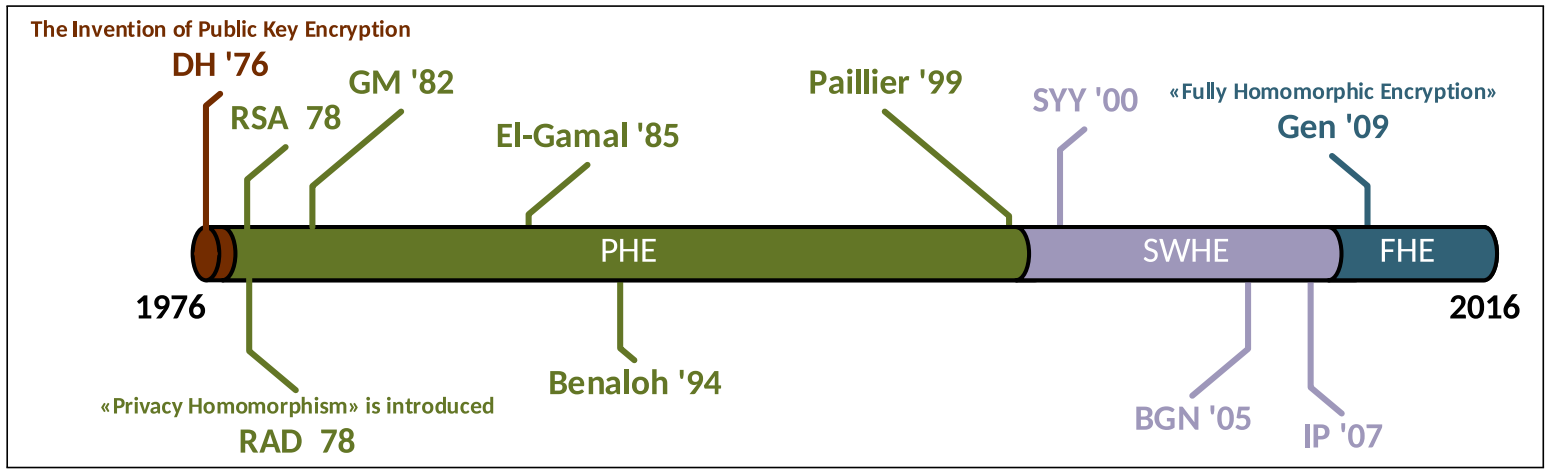
\includegraphics[width=0.8\columnwidth]{./01_body/images/he_timeline.png}
    \caption{Η ιστορική εξέλιξη των Ομομορφικών Σχημάτων μέχρι το πρώτο Πλήρες Ομομορφικό Κρυπτογραφικό Σχήμα \cite{acar2018survey}.}
    \label{fig:he_timeline}
\end{figure}

\subsubsection[Ασφαλής Υπολογισμός Πολλών Μερών (Secure Multi Party Computation ή SMPC)]{Ασφαλής Υπολογισμός Πολλών Μερών (Secure Multi Party \\ Computation ή SMPC)}
Με τον όρο Ασφαλής Υπολογισμών Πολλών Μερών, αναφερόμαστε σε μια κλάση διαδραστικών κρυπτογραφικών σχημάτων η οποία επιτρέπει σε δύο ή περισσότερους συμμετέχοντες που διαθέτουν αντίστοιχες εισόδους (ο κάθε συμμετέχον μπορεί να έχει παραπάνω από μία είσοδο, για χάριν απλότητας όμως μπορούμε να τις θεωρήσουμε ως μια, η οποία μπορεί να ενσωματώνει περισσότερες από μία μέσω κάποιας δομής όπως μια λίστα ή ένα διατεταγμένος ζεύγος), αλλά δεν εμπιστεύονται ο ένας τον άλλον, να υπολογίσουν τις εξόδους μιας συνάρτησης εισάγοντας δημόσια τις από εισόδους τους και εκτελώντας κάποιο κατανεμημένο, ή και μη, πρωτόκολλο. Ο στόχος ενός SMPC πρωτοκόλλου είναι να υπολογίσει σωστά τη συνάρτηση με βάση την είσοδο του κάθε συμμετέχον και να αποκρύψει από κάθε συμμετέχον οποιαδήποτε πληροφορία σχετικά με την είσοδο κάποιου άλλου συμμετέχοντος. Στην περίπτωσή των δύο συμμετεχόντων, αναφερόμαστε ως Ασφαλής Υπολογισμών Δύο Μερών (Secure Two Party Computation ή 2PC). Ο Ασφαλής Υπολογισμός Πολλών Μερών ορίζεται ως εξής :

\begin{definition}
\textbf[Ασφαλής Υπολογισμός Πολλών Μερών (Secure Multi Party Computation ή SMPC)]{Ασφαλής Υπολογισμός Πολλών Μερών (Secure Multi Party Computation ή SMPC)} : Είναι μια κλάση διαδραστικών κρυπτογραφικών σχημάτων που επιτρέπουν σε συμμετέχοντες $P_1, P_2, \dots, P_n$ με αντίστοιχες εισόδους $x_1, x_2, \dots, x_n$ να υπολογίσουν την συνάρτηση την έξοδο $y$ της συνάρτησης $f$, ως $y = f(x_1, x_2, \dots, x_n)$ και ικανοποιούν τις παρακάτω ιδιότητες :

\begin{itemize}
    \item \textbf{Ορθότητα} : Η έξοδος $y$ είναι η σωστή έξοδος της συνάρτησης για τις δεδομένες εισόδους $x_1, x_2, \dots, x_n$
    \item \textbf{Ιδιωτικότητα} : Η έξοδος $y$ είναι η μόνη πληροφορία που φανερώνει το πρωτόκολλο.
\end{itemize}
\end{definition}

Το πρώτο πρωτόκολλο για SMPC παρουσιάστηκε από τον Yao το 1986 στις εργασίες \cite{4568207} \cite{4568388} και προτάθηκε ως πρωτόκολλο επίλυσης του Προβλήματος των Εκατομμυριούχων (\EN{Millionaires' Problem}). Στην βιβλιογραφία σήμερα αναφέρεται ως Μπερδεμένα Δίκτυα Yao (\EN{Yao's Garbled Circuits} ή \EN{Yao's-GC} ή YaoGC). Θα αναλύσουμε το πρωτόκολλο αυτό καθώς και άλλα πρωτόκολλα για SMPC στην Ενότητα \ref{chapter:SMPC}.
\chapter{Κρυπτογραφία}
\label{chapter:cryptography}

Στο κεφάλαιο αυτό θα γίνει μια εισαγωγή στην Κρυπτογραφία. Αρχικά θα αναλύσουμε βασικούς ορισμούς/μοντέλα κρυπτογραφικών σχημάτων, ξεκινώντας από πιο ιστορικούς και καταλήγοντας σε πιο σύγχρονους. Πολλοί από αυτούς θα χρησιμοποιηθούν στην Ενότητα \ref{chapter:security} ως βασικά δομικά στοιχεία. Στην συνέχεια του κεφαλαίου θα αναλύσουμε κυρίως σύγχρονα κρυπτογραφικά εργαλεία και πρωτόκολλα που χρησιμοποιούνται ως συστατικά στοιχεία σε σύγχρονα πρωτόκολλα και πολλά από αυτά θα χρησιμοποιηθούν ως βασικά δομικά στοιχεία στις Ενότητες \ref{chapter:SMPC} και \ref{chapter:implementation}. Σε καμία περίπτωση αυτή η Ενότητα δεν αποτελεί μια πλήρη εισαγωγή στον κλάδο της κρυπτογραφίας. ο αναγνώστης που ενδιαφέρεται για κάτι τέτοιο μπορεί να απευθυνθεί στα βιβλία \cite{boneh2020graduate}, \cite{hoffstein2008introduction}, \cite{pagourtzis2016computational}, το τελευταίο εκ των οποίων είναι και στην ελληνική γλώσσα.

\section{Βασικοί Ορισμοί}

\subsection{Πρωταρχικοί Ορισμοί}

Αρχικά θα αναφερθούμε στους πρώτους ιστορικά τυποποιημένους ορισμούς κρυπτογραφικών σχημάτων που έγιναν από τον Shannon, οι οποίοι αναφέρονται σε συστήματα συμμετρικής κρυπτογραφίας, με απώτερο σκοπό να μπορέσουμε να παρουσιάσουμε με σαφήνεια τα μοντέλα των αντιπάλων, της ασφάλειας και των αποδείξεων τους στην Ενότητα \ref{chapter:security}. Αυτά στην συνέχεια μπορούν να γενικευθούν, να προσαρμοστούν και να χρησιμοποιηθούν σε όλα τα κρυπτογραφικά κατασκευάσματα, όπως αυτά της ασύμμετρης κρυπτογραφίας, των συναρτήσεων κατακερματισμού, των κρυπτογραφικών πρωτοκόλλων κ.α.

Ο Shannon στην εργασία \cite{shannon1945mathematical} όρισε το παρακάτω γενικό μαθηματικό μοντέλο συμμετρικού κρυπτογραφικού σχήματος.

\begin{definition}
\label{def:shannon_cipher}
\textbf{Κρυπτογραφικό Σχήμα Shannon (Shannon Cipher)} : Ένα ζεύγος ντετερμινιστικών συναρτήσεων $\mathcal{E} = (\enc, \dec)$ οι οποίες ορίζονται ως εξής:
\begin{itemize}
    \item $\enc$ : $\mathcal{K} \times \mathcal{M} \rightarrow \mathcal{C}$
    \item $\dec$ : $\mathcal{K} \times \mathcal{C} \rightarrow \mathcal{M}$
\end{itemize}
όπου $\mathcal{M}$, $\mathcal{C}$, $\mathcal{K}$ είναι οι χώροι των μηνυμάτων, κρυπτοκειμένων και κλειδιών αντίστοιχα τους οποίους θα θεωρήσουμε πεπερασμένους. Στην περίπτωση αυτή λέμε ότι το κρυπτοσύστημα $\mathcal{E}$ ορίζεται πάνω στο $(\mathcal{K},\mathcal{M},\mathcal{C})$. Οι συναρτήσεις $\enc, \dec$ ορίζονται ως εξής:

\begin{itemize}
    \item H $\enc$ είναι η συνάρτηση κρυπτογράφησης και παίρνει ως όρισμα ένα κλειδί $k \in \mathcal{K}$ και ένα μήνυμα $k \in \mathcal{M}$ και επιστρέφει ένα κρυπτοκείμενο $c \in \mathcal{C}$. Δηλαδή :
    $$
    c = \enc_k(m) \text{ ή με ισοδύναμο συμβολισμό } c = \enc(k, m)
    $$
    \item H $\dec$ είναι η συνάρτηση αποκρυπτογράφησης, δηλαδή η αντίστροφη συνάρτηση της \enc, και παίρνει ως όρισμα ένα κλειδί $k \in \mathcal{K}$ και ένα κρυπτοκέιμενο  $c \in \mathcal{C}$ και επιστρέφει ένα μήνυμα $m \in \mathcal{M}$. Δηλαδή : 
    $$
    m = \dec_k(c) \text{ ή με ισοδύναμο συμβολισμό } m = \dec(k, c)
    $$
\end{itemize}
    Όπου οι $\enc$, $\dec$ ακολουθούν την παρακάτω Ιδιότητα Ορθότητας:
    \begin{equation}
    \label{shannon_decryption_identity}
    \forall m \in \mathcal{M}, \forall k \in \mathcal{K} : Pr[m = \dec_k(\enc_k(m))] = 1
    \end{equation}
\end{definition}

Ένα παράδειγμα Κρυπτογραφικού Σχήματος Shannon είναι αυτό του Σημειωματάριου Μιας Χρήσης (One Time Pad ή OTP) \cite{miller1882telegraphic} με σταθερό ή και μεταβλητό μήκος $m$ και $c$. 

Δυστυχώς, ο Ορισμός \ref{def:shannon_cipher} είναι πολύ γενικός και η κλάση των κρυπτογραφικών σχημάτων που ορίζει, συμπεριλαμβάνει προβλήματα με μη πρακτικές χρονικές και χωρικές πολυπλοκότητες. Έτσι, υπήρξε ανάγκη στην βιβλιογραφία να συμπεριληφθεί μια ακόμα κλάση κρυπτογραφικών σχημάτων που συμπεριλαμβάνει, αποκλειστικά, κρυπτογραφικά σχήματα που μπορούν να υλοποιηθούν αποδοτικά.

\begin{definition}
\label{def:computational_cipher}
\textbf{Υπολογιστικό Κρυπτογραφικό Σχήμα (Computational Cipher) \cite{boneh2020graduate}} : Ένα ζεύγος συναρτήσεων $\mathcal{E} = (\enc, \dec)$ όπως ορίζονται στο Κρυπτογραφικό Σχήμα Shannon υπό τον περιορισμό ότι οι αλγόριθμοι $\enc$, $\dec$ είναι αποδοτικοί και πιθανοτικοί δηλαδή, $\enc, \dec \in PPT(\secparam)$, όπου $\secpar$ παράμετρος ασφάλειας, διατηρώντας την Ιδιότητα Ορθότητας \ref{shannon_decryption_identity}.
\end{definition}

Σήμερα για την ασφαλή ανταλλαγή μηνυμάτων διακρίνονται δύο κύριες κατηγορίες Υπολογιστικών Κρυπτογραφικών Σχημάτων. Τα Συμμετρικά και Ασύμμετρα Κρυπτογραφικά σχήματα, με την λέξη "Υπολογιστικά" να παραλείπεται και να αναφέρεται μόνο όπου υπάρχει ανάγκη διάκρισης από άλλα σχήματα, αφού κυρίως μας ενδιαφέρουν πρακτικά σχήματα και σε αυτά θα επικεντρωθούμε και στα πλαίσια αυτής της εργασίας.

\subsection{Συμμετρική Κρυπτογραφία}

Η συμμετρική κρυπτογραφία παίρνει το όνομά της από την συμμετρική χρήση κλειδιών, δηλαδή το ίδιο κλειδί που θα χρησιμοποιηθεί για την κρυπτογράφηση θα πρέπει να χρησιμοποιηθεί και για την αποκρυπτογράφηση. Στην κατηγορία των συμμετρικών κρυπτογραφικών σχημάτων ανήκουν τα περισσότερα σχήματα και συστήματα της Κλασσικής Κρυπτογραφίας.

\begin{definition}
\label{def:symetric_cryptographic_scheme}
\textbf{Συμμετρικό Κρυπτογραφικό Σχήμα (\EN{Symmetric Cryptographic \\ Scheme})} : Έστω κατάλληλα $\mathcal{M}$, $\mathcal{C}$, $\mathcal{K}$. Αποτελείτε από ένα σύνολο αποδοτικών αλγορίθμων $(\kgen, \enc, \dec)$ οι οποίοι ορίζονται παρόμοια με τον Ορισμό \ref{def:computational_cipher} και έχουν τις εξής λειτουργίες :
\begin{itemize}
    \item $k \leftarrow \kgen(1^\secpar)$ : Δημιουργεί ένα κρυπτογραφικό κλειδί $k$ το οποίο χρησιμοποιείται τόσο για κρυπτογράφηση όσο και για αποκρυπτογράφηση.
    \item $c \leftarrow \enc_{k}(m)$ : Κρυπτογραφεί ένα μήνυμα $m$ χρησιμοποιώντας το κλειδί $k$.
    \item $m \leftarrow \dec_{k}(c)$ : Αποκρυπτογραφεί ένα κρυπτοκείμενο $c$ χρησιμοποιώντας το κλειδί $k$.
\end{itemize}
Οι παραπάνω αλγόριθμοι πρέπει να ακολουθούν την εξής Ιδιότητα Ορθότητας όπως ακριβώς και με τον Ορισμό \ref{def:computational_cipher}.
\end{definition}

Ένα από τα βασικότερα μειονεκτήματα των συμμετρικών κρυπτογραφικών σχημάτων είναι ότι στην περίπτωση που χρησιμοποιούνται για ασφαλή επικοινωνία για κάθε συμμετέχοντα που θέλει να συμμετάσχει στην επικοινωνία θα πρέπει ο κάθε συμμετέχοντας να διαθέτει για την επικοινωνία τους ένα μοναδικό κλειδί. Δηλαδή στην περίπτωση των $n$ συμμετεχόντων θα χρειαστούμε $n^2$ κλειδιά, το πρόβλημα αυτό είναι γνωστό και ως \textbf{Πρόβλημα των Τετραγώνων στην βιβλιογραφία}. Έτσι τα σχήματα αυτά, από μόνα τους, καθίστανται ανίκανα για χρήση σε μεγάλα δίκτυα επικοινωνίας, όπως το Διαδίκτυο ή το Διαδίκτυο των Πραγμάτων. Ένα ακόμη μειονέκτημα είναι ότι οι συμμετέχοντες θα πρέπει να έχουν προαποφασίσει ένα συμμετρικό το συμμετρικό τους κλειδί. Τα προβλήματα αυτά έλυσε η εφεύρεση της ασύμμετρης κρυπτογραφίας. Τέλος σημαντικό είναι να αναφέρουμε ότι αυτά τα κρυπτογραφικά σχήματα λόγω του μεγάλου τους πλεονεκτήματος να έχουν πολύ γρήγορες υλοποιήσεις χρησιμοποιούνται κατά κόρον για μεταφορά μεγάλου όγκου δεδομένων.

\subsection{Ασύμμετρη Κρυπτογραφία}

Η ιστορία της Ασύμμετρης Κρυπτογραφίας αναφέρθηκε την Ενότητα \ref{chapter:intro}. Ο ορισμός των αντίστοιχων κρυπτογραφικών σχημάτων είναι παρόμοιος με αυτόν των συμμετρικών, με την κύρια διαφορά ότι υπάρχει ένα ζεύγος κλειδιών, το δημόσιο και το ιδιωτικό. Ο αυστηρώς ορισμός της παρουσιάζεται παρακάτω :

\begin{definition}
\label{def:assymetric_cryptographic_scheme}
\textbf{Ασυμμετρικό Κρυπτογραφικό Σχήμα (\EN{Assymetric Cryptographic \\ Scheme})} : Ορίζεται παρόμοια με τον Ορισμό \ref{def:symetric_cryptographic_scheme} με μοναδική διαφορά το ζέυγος κλειδιών και την ιδιότητα ορθότητας. Αποτελείτε από ένα σύνολο αλγορίθμων $(\kgen, \enc, \dec)$ με τις εξής λειτουργίες :
\begin{itemize}
    \item $(pk, sk) \leftarrow \kgen(1^\secpar)$ : Δημιουργεί ένα ζεύγος ασύμμετρων κρυπτογραφικά κλειδιών. Το Δημόσιο Κλειδί (Public Key) $pk$ που χρησιμοποιείται στην κρυπτογράφηση και το αντίστοιχο Ιδιωτικό Κλειδί (Private Key) $sk$ που χρησιμοποιείται στην αποκρυπτογράφηση.
    \item $c \leftarrow \enc_{pk}(m)$ : Κρυπτογραφεί ένα μήνυμα $m$ χρησιμοποιώντας το δημόσιο κλειδί $pk$.
    \item $m \leftarrow \dec_{sk}(c)$ : Αποκρυπτογραφεί ένα κρυπτοκείμενο $c$ χρησιμοποιώντας το ιδιωτικό κλειδί $sk$.
\end{itemize}
Όπως και στην περίπτωση της Συμμετρικής Κρυπτογραφίας οι παραπάνω αλγόριθμοι πρέπει να ακολουθούν την εξής ιδιότητα ορθότητας :
$$
    Pr(\dec_{sk}(\enc_{pk}(m))) = Pr(\enc_sk(\enc_pk{m})) = 1
$$
\end{definition}

Η τελευταία, ιδιότητα δηλαδή ότι $\dec_pk(m)=\enc^{-1}_sk(m)$ δίνει και την δυνατότητα για την υποστήριξη ψηφιακών υπογραφών και αποστολής μηνυμάτων με ένα ζεύγος κλειδιών ανά συμμετέχοντα.

Η Ασύμμετρη Κρυπτογραφία λύνει το πρόβλημα της διανομής κρυπτογραφικών κλειδιών που υπάρχει στην περίπτωση της Συμμετρικής, καθότι ο κάθε συμμετέχων χρειάζεται να διαθέτει μόνο ένα ζεύγος κλειδιών, από τα οποία το ένα μπορεί να το μοιραστεί δημόσια. Επίσης, μπορεί να χρησιμοποιηθεί ως συστατικό στοιχείο σε πολλά πρωτόκολλα με σκοπούς πέραν της απλής ανταλλαγής μηνυμάτων και των ψηφιακών υπογραφών, που θα ήταν αδύνατα χωρίς την ασύμμετρη κρυπτογραφία. Ωστόσο, αν και πρόκειται για σύγκριση ανόμοιων πραγμάτων, τα ασύμμετρα κρυπτογραφικά σχήματα είναι πιο κοστοβόρα (αρκετές δεκάδες φορές για μικρό μέγεθος μηνυμάτων και εώς και μια τάξη μεγέθους για μεγάλο μέγεθος μηνυμάτων) σε σχέση με τα συμμετρικά από άποψη υπολογισμών και πόρων στις υλοποιήσεις τους. Ένα απλό παράδειγμα φαίνεται στο Σχήμα \ref{code:rsa_vs_aes}\footnote{Είναι σημαντικό αναφέρουμε ότι σχεδόν όλοι οι σύγχρονοι CISC επεξεργαστές διαθέτουν εξειδικευμένα κυκλώματα καθώς και αντίστοιχες εντολές μηχανής και συμβολική γλώσσας για το κρυπτογραφικό σχήμα AES κάτι που σε καμία περίπτωση δεν ισχύει για τον RSA. Το τελευταίο οφείλεται και στο ότι η φύση τελευταίου δεν επιδέχεται μεγάλο βαθμό παραλληλοποίησης.} στο οποίο συγκρίνονται οι χρόνοι (cpu time) κρυπτογράφησης και αποκρυπτογράφησης ενός μικρού μηνύματος για τα σχήματα RSA και AES. Έτσι, σήμερα σεαρκετά δημοφιλή κρυπτογραφικά πρωτόκολλα, όπως για παράδειγμα στο πρωτόκολλο TLS \cite{RFC8446}, που χρησιμοποιείται για την ασφαλή επικοινωνία στο Επίπεδο Μεταφοράς ενός δικτύου, στην αρχή της συνεδρίας χρησιμοποιούνται ασυμμετρικά σχήματα ψηφιακών υπογραφών και ανταλλαγής κλειδιών, όπως τα ECDSA και ECDHE αντίστοιχα, με σκοπό την δημιουργία από κοινού συμμετρικών κλειδιών που χρησιμοποιούνται στην συνέχεια από συμμετρικούς αλγορίθμους για την κρυπτογράφηση των δεδομένων της επακόλουθης συνεδρίας. Ακόμα, ένα από τα κύρια χαρακτηριστικά των ασυμμετρικών σχημάτων είναι ότι πιο μαθηματικά δομημένα. Αυτό έχει ως αποτέλεσμα συνήθως να βασίζονται έμμεσα σε πιο πολύπλοκους μαθηματικούς υπολογισμούς, όπως η εύρεση μεγάλων πρώτων αριθμών σε σχέση με τους σχετικά απλούς υπολογισμούς που εκτελεί ένα συμμετρικό σχήμα. Μια ακόμα συνέπεια του χαρακτηριστικού τους ότι είναι πιο μαθηματικά δομημένα, είναι ότι η ασφάλεια τους κατά κόρον βασίζεται σε υποθέσεις πολυπλοκότητας, όπως αυτές που θα αναφερθούν στην Ενότητα \ref{chapter:security}, από τις οποίες πολλές από αυτές έχει αποδειχθεί ότι δεν ισχύουν σε μη κλασσικά μοντέλα υπολογισμού, όπως το κβαντικό, αλλά και κάνουν την απόδειξη της ασφάλειας τους πιο πολύπλοκη.

\begin{figure}[h]
    \begin{center}
        \inputminted[fontsize=\scriptsize,frame=single]{python}{./01_body/code/rsa-vs-aes.py}
        \inputminted[fontsize=\scriptsize,frame=single]{text}{./01_body/code/rsa-vs-aes.output}
    \end{center}
    \caption{Μικρή σύγκριση των επιδόσεων για την κρυπτογράφηση και την αποκρυπτογράφηση ενός απλού μηνύματος μεταξύ συμμετρικών και ασύμμετρων κρυπτογραφικών σχημάτων (AES, RSA).}
    \label{code:rsa_vs_aes}
\end{figure}

\section{Κρυπτογραφικά Εργαλεία}

Στην Ενότητα αυτή θα μελετήσουμε σύγχρονα κρυπτογραφικά εργαλεία που αποτελούν βασικά συστατικά στοιχεία πολλών Κρυπτογραφικών Προτοκόλλων με διάφορες εφαρμογές. Πολλά από αυτά παρατηρούνται συχνά σε πρωτόκολλα SMPC κάτι που θα το παρατηρήσουμε πρακτικά και στο Κεφάλαιο \ref{chapter:SMPC}.

\subsection{Σχήματα Δέσμευσης (Commitment Schemes)}

Τα Σχήματα Δέσμευσης (Commitment Schemes) είναι το πρώτο εργαλείο που θα εξετάσουμε. Αυτά έχουν τη μορφή πρωτοκόλλων επικοινωνίας δύο φάσεων μεταξύ δύο (ή πιο σπάνια περισσότερων) συμμετεχόντων. Παρέχουν την δυνατότητα σε έναν συμμετέχον, $S$, να δεσμευτεί κάποια συγκεκριμένη τιμή σε κάποιον άλλον, $R$, χωρίς όμως αυτός να γνωρίζει ο $S$ την συγκεκριμένη τιμή, δηλαδή η τιμή είναι σε κρυπτογραφημένη μορφή. Το πρωτόκολλο δίνει την δυνατότητα να αποκαλυφθεί στον $R$ η τιμή στην οποία δεσμεύτηκε αρχικά ο $V$, και μόνο αυτή, σε επόμενη χρονική στιγμή την οποία επιλέγει ο συμμετέχον $S$. Αυτό αποτρέπει τον συμμετέχον $S$ στο να μεταβάλλει την τιμή αυτή χωρίς να γίνει αντιληπτό από τον άλλο συμμετέχον. Τα σχήματα αυτά χρησιμοποιούνται ως δομικά στοιχεία σε σχήματα Αποδείξεων Μηδενικής Γνώσης αλλά και στον Ασφαλή Υπολογισμό. Το Σχήμα Δέσμευσης ορίζεται ως εξής :

\begin{definition}
    \textbf{Σχήματα Δέσμευσης} : Έστω $Μ$ ο χώρος των μηνυμάτων, $C$ ο χώρος των δεσμευμένων τιμών, $D$ ο χώρος των κλειδιών αποδέσμευσης και $R$ μια ομοιόμορφη πιθανοτική κατανομή που περιέχει αρκετή εντροπία για οποιοδήποτε σχήμα δέσμευσης. Τα σχήματα δέσμευσης είναι πρωτόκολλα δύο συμμετεχόντων, $S$ και $R$, στα οποία ο $S$ δεσμέυετε μια τιμή στον $R$. Αποτελούνται από μια τριάδα αλγορίθμων $(\text{Setup}, \text{Commit}, \text{Verify})$ που ορίζονται ως εξής :
    \begin{itemize}
        \item $\text{Setup}(\secparam)$ :
        \item $\text{Commit}(m, r)$ : Δέχεται ως όρισματα ένα μήνυμα $m$ και μερικά τυχαία νομίσματα $r$, και δίνει ως εξόδους μια δεσμευμένη τιμή $c$ και ένα κλειδί αποδέσμευσης $d$ για την $c$.
        \item $\text{Open}(c, m, d)$ : Δέχεται ως όρισματα μια δεσμευμένη τιμή $c$, το μήνυμα $m$ και το κλειδί ανοίγματος $d$, και δίνει ως έξοδο μια δυαδική τιμή ανάλογα με το αν η τιμή που φανερώθηκε από την αποδέσμευση της $c$ μέσω της $d$ είναι η $m$.
    \end{itemize}
    Το σχήμα πρέπει να ικανοποιεί τις παρακάτω ιδιότητες :
    \begin{itemize}
        \item \textbf{Ορθότητα (Completeness)} : $\forall m \in M, r \sample R : Pr[\text{Open}(\text{Commit}(m, r), m)] = 1$
        \item \textbf{Απόκρυψη (Hiding)} : $\forall \text{ distinct } m, m' \in M, r \sample \text{R}, \forall A :\\
         \abs{Pr[A(\text{Commit}(m, r))] - Pr[A(\text{Open(r, m')})]} \leq ε_h$
        \item \textbf{Δέσμευση (Binding)} : $\forall \text{ distinct } m, m', \forall \text{ distinct } d, d', \forall c :\\
         \abs{Pr[\text{Open}(c, m, d)] - Pr[\text{Open}(c, m', d')]} \leq ε_b$
    \end{itemize}
\end{definition}

Οι τιμές $ε_h$ και $ε_b$ εξαρτόνται από το είδος της ιδιότητας που θέλουμε να έχουμε. Σε αντιστοιχία με τους ορισμούς ασφάλειας αλλά και με την ισχύ του αντιπάλου που θα ορίσουμε στο επόμενο κεφάλαιο, μπορούμε να έχουμε \textbf{Υπολογιστική}, \textbf{Στατιστική} ή \textbf{Τέλεια} \textbf{Απόκρυψη} και \textbf{Δέσμευση} και οι τιμές που λαμβάνουν οι $ε_h$ και $ε_b$ είναι $0$, $negl(\secparam)$ και  $negl(\secparam)$ αντίστοιχα. Τέλος, μπορεί να αποδειχθεί σχετικά εύκολα, ότι δεν μπορούμε να έχουμε σχήματα που να διαθέτουν ταυτόχρονα τέλεια απόκρυψη και τέλεια δέσμευση.

\subsection{Αποδείξεις Μηδενικής Γνώσης}

Το επόμενο εργαλείο που θα εξετάσουμε είναι αυτό τον Αποδείξεων Μηδενικής Γνώσης. Η Μηδενική Γνώση είναι μια ιδιότητα που μπορεί να αποκτήσει η κλάση $\IP$ των Διαδραστικών Αποδείξεων αν υποθέσουμε ότι υπάρχουν Συναρτήσεις Μονής Διαδρομής (One Way Functions ή OWF), μια υπόθεση που θα δούμε στο επόμενο κεφάλαιο. Στο Κεφάλαιο \ref{chapter:appendix} κάνουμε μια μικρή μελέτη στις διαδραστικές αποδείξεις που είναι άμεσα συσχετισμένες με τις Αποδείξεις Μηδενικής Γνώσης. Διαισθητικά σε ένα πρωτόκολλο με την ιδιότητα αυτή ο Αποδεικνύων $P$, μπορεί να αποδείξει στον Επαληθευτή $V$ ότι γνωρίζει κάποιον μάρτυρα $w$ που ανήκει σε μια προκαθορισμένη γλώσσα $L$ που γνωρίζουν και οι δύο οντότητες, χωρίς ο $V$ να μπορεί να αποκτήσει γνώση σχετικά με τον $w$. Μια πιο παραστατική αντίληψη του πως λειτοργούν οι αποδείξεις με την ιδιότητα αυτή παρουσιάζεται στο Σχήμα \ref{fig:zero_knowledge_comic}. Σχετικά με τον αυστηρό ορισμό της ιδιότητας της Μηδενικής Γνώσης, χρειάστηκαν αρκετά χρόνια ώστε να υπάρξει ένας καταληκτικός ορισμός στη βιβλιογραφίας. Αυτός παρουσιάζεται παρακάτω σε αντιστοιχία με τον ορισμό της κλάσης IP:

\begin{figure}[ht]
    \centering
    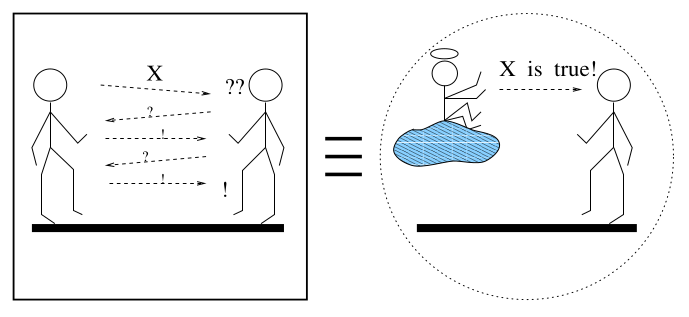
\includegraphics[width=10cm]{./01_body/images/zero_knowledge_comic.png}
    \caption{Κόμικ που αναπαρηστά πως λειτουργούν οι Αποδείξεις Μηδενικής Γνώσης \cite{goldreich2013short}.}
    \label{fig:zero_knowledge_comic}
\end{figure}

\begin{definition}
\label{def:czk}
\textbf{Κλάση Αποδείξεων Μηδενικής Γνώσης (\EN{Computational Zero Knowledge Proofs} ή $\CZK$)} : Έστω $P$ ντετερμινιστική συναρτήση ΤΜ που είναι απεριόριστης ισχύος. Η γλώσσα $L$ λέμε ότι ανήκει στην κλάση $\IP$, δηλαδή $L \in IP$ αν υπάρχει μη ντετερμινιστική ΤΜ $V$ με $x, r, a_{1}, \ldots, a_{i}, V$ και χρονική πολυπλοκότητα σε $O(poly(|x|))$ που ικανοποιεί τις παρακάτω ιδιότητες :s
\begin{itemize}
    \item \textbf{Πληρότητα (Completeness)} : $x \in L \Rightarrow \exists \operatorname{Pr}\left[\text { out }_{V}\langle V, P\rangle(x)=1\right] \geq (ε=) \dfrac{2}{3}$
    \item \textbf{Ορθότητα (Soundness)} : $x \notin L \Rightarrow \forall \operatorname{Pr}\left[\text { out }_{V}\langle V, P\rangle(x)=1\right] \leq 1 - ε$
    \item \textbf{Μηδενική Γνώση} : $\forall V, \exists S \in PPT : \forall x \in L \wedge w \in R_L$ :
    $$
    View_V = S(x,z)
    $$
\end{itemize}
\end{definition}

Προφανώς όπως ισχύει και για τις ιδιότητες της Πληρότητας και της Ορθότητας των Διαδραστικών Αποδείξεων έτσι και για την ιδιότητα της Μηδενικής Γνώσης μπορούμε να έχουμε από τους αντίστοιχους ορισμούς ασφάλειας που θα παρουσιαστούν στο επόμενο κεφάλαιο, \textbf{Τέλεια}, \textbf{Στατιστική} ή \textbf{Υπολογιστική Μηδενική Γνώση} ανάλογα με τον τύπο της δυσδιακριτότητας των κατανομών της μηδενικής γνώσης και οι κλάσεις που ορίζουν είναι οι $PZK$, $SZK$ και $CZK$ αντίστοιχα. Για τις κλάσεις αυτές γνωρίζουμε ότι $\PZK \subseteq \SZK \subseteq \CZK$. Η ευρύτερη από αυτές τις κλάσεις είναι αυτή της $\CZK$ που παρουσιάστηκε και στον Ορισμό \ref{def:czk}. Για την κλάση $\CZK$ γνωρίζουμε ότι $\IP=\CZK=\PSPACE$ και ότι $\NP \subseteq \CZK$, προφανώς υπό την υπόθεση OWF \cite{ben1988everything}. Για τις κλάσεις $\SZK$ και $\PZK$ ωστόσο δεν έχει αποδειχθεί κάποια παρόμοια ισότητα αλλά γνωρίζουμε το εξής $\PZK \subseteq \SZK \subseteq \AM \cap \coAM$ και επίσης εικάζεται ότι δεν ισχύει $NP \subseteq \SZK$ καθώς τότε καταρρέει όλη η πολυωνυμική ιεραρχία της $\NP$. Μια σύνοψη της γνώσης που έχουμε προς το παρόν για τις τρεις προηγούμενες κλάσεις, συμπεριλαμβανομένων και αρκετών σχέσεων που παραλήψαμε για λόγους συνοπτικότητας, μπορεί να βρεθεί στην εργασία \cite{couteau2017zero}. Δεν μπορούμε να παραλείψουμε να αναφέρουμε δύο σημαντικές κλάσεις που σχετίζονται άμεσα με την $CZK$, αυτή των Μη Διαδραστικών Αποδείξεων Μηδενικής Γνώσης, $NICZK$, και αυτή των Πιθανοτηκά Ελεγχόμενων Αποδείξεων $\PCP$, ωστόσο η μελέτη τους εμπείπτει εκτός τον σκοπώς αυτής της εργασίας.

Παρακάτω παρουσιάζεται ένα από τα πιο γνωστά σχήματα μηδενικής γνώσης, το Πρωτόκολλο Schnorr που μπορεί να χρησιμοποιηθεί για να αποδειχθεί η γνώση μιας λύσης ενός στιγμιοτύπου του προβλήματος του Διακριτού Λογαρίθμου, δηλαδή ενός στοιχείου $x$ τέτοιου ώστε $h=g^x$.

\begin{definition}
    \textbf{Πρωτόκολλο Schnorr : Απόδειξη Μηδενικής Γνώσης για τον Διακριτό Λογάριθμο} \cite{cramer1994proofs} :
    Έστω μια πολλαπλασιαστική ομάδα $G$, πρώτης τάξης με $\abs{G}=q$.
    \begin{itemize}
        \item \textbf{Εισόδοι} :
            \begin{itemize}
                \item $P$ : $x$, $h$
                \item $V$ : $h$
            \end{itemize}
        \item \textbf{Πρωτόκολλο} : 
            \pcb {
                P \< \< V \\ [][\hline]
                r \sample \mathbb{Z_q} \< \< \\
                u \gets g^r \< \< \\
                \< \sendmessageright*{u} \< \\
                \< \< c \sample \mathbb{Z}_q \\
                \< \sendmessageleft*{c} \< \\
                z \gets r + cx \< \< \\
                \< \sendmessageright*{z} \< \\
                \< \< g^z \stackrel{?}{=} u \cdot h^c
            }
        \item \textbf{Εξόδοι} :
            \begin{itemize}
                \item $P$ : $\perp$
                \item $V$ : $0$ ή $1$ ανάλογα με το αν ισχύει η τελευταία πράξη ισότητας που εκτέλεσαι
            \end{itemize}
    \end{itemize}
\end{definition}

\subsection{Σχήματα Ανυποψίαστης Μεταφοράς}

Τα σχήματα Ανυποψίαστης Μεταφοράς (Oblivious Transfer ή OT) είναι το επόμενο κρυπτογραφικό εργαλείο που θα μελετήσουμε.Πρόκειται πρωτόκολλα δύο συμμετεχόντων, $P_1$, $P_2$, στα οποία ο ένας συμμετέχον έχει $n$ τιμές και από τις οποίες ο άλλος συμμετέχον μπορεί να επιλέξει $t \le n$ από αυτές δίχως ο πρώτος συμμετέχον να γνωρίζει ποιες επέλεξε ο δεύτερος. Ίσως να ακούγεται ανόητη η χρησιμότητα τους όμως έχει αποδειχθεί ότι έχουν πολύ μεγάλη σημασία και δίχως σχήματα OT πολλά σύνθετα δεν μπορούν να υλοποιηθούν. Για να αντιληφθούμε την σημασία τους, έχει αποδειχθεί πως με βάση μόνο σχήματα OT μπορεί να υπολογιστεί οποιαδήποτε SMPC συνάρτηση \cite{10.1561/3300000019}. Το πρώτο πρωτόκολλο Ανυποψίαστης Μεταφοράς παρουσιάστηκε στην βιβλιογραφία το 1981 από τον Rabin, στην εργασία \cite{cryptoeprint:2005/187}. Μπορούμε να μοντελοποιήσουμε τα σχήματα αυτά ως εξης :

\begin{definition}
\textbf{Πρωτόκολλο Ανυποψίαστης Μεταφοράς t από τα n (Oblivious Transfer ή ΟΤ t-out-of-n)} :
\begin{itemize}
    \item \textbf{Εισόδοι} :
        \begin{itemize}
            \item $P_1$ : $b_{0}, b_{1}, \ldots b_{n} \in \bin^l$
            \item $P_2$ : $t_{0}, t_{1}, \ldots t_{n} \in \bin$
        \end{itemize}
    \item \textbf{Εξόδοι} :
        \begin{itemize}
            \item $P_1$ : $\perp$
            \item $P_2$ : \{$\forall t_n : b_{\{t_n = 1\}}\}$
        \end{itemize}
\end{itemize}
\end{definition}

Πολλές φορές στην βιβλιογραφία χρησιμοποιείται ο συμβολισμός OT t/n ή OT t-n, δηλαδή για παράδειγμα OT 1-2 ή OT 1/2. Παρακάτω παρουσιάζεται ένα πρωτόκολλο για OT 1-2 που είναι Σημασιολογικά Ασφαλές απέναντη σε Παθητικούς Αντιπάλους και παρουσιάστηκε στην εργασία \cite{even1985randomized}.

\begin{definition}
\label{def:oblivious_transfer}
\textbf{Πρωτόκολλο Ανυποψίαστης Μεταφοράς 1/2 (Oblivious Transfer 1/2)} \cite{even1985randomized} : 
\begin{itemize}
\item \textbf{Εισόδοι} : 
    \begin{itemize}
    \item Κοινή είσοδος : Οικογένεια Trapdoor Permutations (TDP) : $(I, S, F, F^{-1})$, Hardcore Predicate : $B$
    \item $P_{1}$ : $b_{0}, b_{1} \in\{0,1\}$
    \item $P_{2}$ : $\sigma \in\{0,1\}$.
    \end{itemize}
\item \textbf{Πρωτόκολλο} : \\
    \pcb {
    P_1 \< \< P_2 \\ [][\hline]
    (a, τ) \gets I(\secparam) \< \< \\
    \< \sendmessageright*{(a, t)} \> \\
    \< \< x_σ \gets S(a) \\
    \< \< y_{1-σ} \gets S(a) \\
    \< \< y_{σ} \gets F(a, x_s) \\
    \< \sendmessageleft*{y_0, y_1} \< \\
    x_0 \gets F^{-1}(a, y_0) \< \< \\
    x_1 \gets F^{-1}(a, y_1) \< \< \\
    β_0 \gets B(a, x_0) \oplus b_0 \< \< \\
    β_1 \gets B(a, x_1) \oplus b_1 \< \< \\
    \< \sendmessageright*{β_0, β_1} \< \\
    \< \< b_σ \gets B(a, x_σ) \oplus β_σ
    }

\item \textbf{Εξόδοι} :
    \begin{itemize}
        \item $P_1$ : $\perp$
        \item $P_{2}$ : $b_σ$
    \end{itemize}
\end{itemize}
\end{definition}

\subsection{Σχήματα Διαμοίρασης Μυστικών (Secret Sharing)}

Το τελευταίο κρυπτογραφικό εργαλείο που θα μελετήσουμε είναι αυτό των σχημάτων Διαμοίρασης Μυστικών. Για να αντιληφθούμε τη χρησιμότητα των σχημάτων Διαμοίρασης Μυστικών ας εξετάσουμε πρώτα ένα απλό παράδειγμα. Ας υποθέσουμε ότι ο ιδιοκτήτης μιας επιχείρησης έχει στην κατοχή του κάποια πολύ σημαντικά έγγραφα τα οποία βρίσκονται σε κάποια θυρίδα που είναι ασφαλισμένη με κάποιο κωδικό. Σε αυτά τα έγγραφα θέλει να έχει πρόσβαση το Διοικητικό Συμβούλιο της εταιρίας ακόμα και στην περίπτωση που αυτός δεν είναι παρόν, π.χ. στην περίπτωση που αυτός ξαφνικά φύγει από την ζωή, υπό την προϋπόθεση όμως ότι η πλεοψηφία, ή κάποιο συγκεκριμένο ποσοστό που έχει επιλέξει αυτός,των συμβούλων συμφωνεί στο άνοιγμα της θυρίδας. 

Το πρώτο κρυπτογραφικό σχήμα που λύνει το πρόβλημα αυτό παρουσιάστηκε από τον Shamir στην εργασία \cite{10.1145/359168.359176} το 1979 και σήμερα απαντάται στην βιβλιογραφία ως Πρωτόκολλο Διαμοίρασης Μυστικών Shamir. Βασίζεται στο γεγονός ότι οποιοδήποτε σύνολο $n+1$ σημείων σε ένα δυδιάστατο πεδίο $\mathbf{F}^2$ καθορίζει μοναδικά ένα πολυώνυμο $n$ βαθμού. Δηλαδή αν $f:\mathbb{F} \rightarrow \mathbb{F}$ όπου $f(x)=\pn{α}{x}$ τότε ένα σύνολο σημείων $(x_i, f(x_i))$ όπου $x \in [0, n]$ είναι επαρκές για να ανακτήσουμε την συνάρτηση $f$. Αυτό μπορεί πολύ εύκολα να συμβεί λύνοντας το σύστημα εξισώσεων μεγέθους $(n+1) \cdot (n+1)$ που προκύπτει αν αντικαταστήσουμε με κάθε σημείο την γενική εξίσωση πολυωνύμου $f(x_i)=\pn{a}{x_i}$. Ένας πιο εύκολος τρόπος να επιτευχθεί αυτό είναι μέσω των πολλαπλασιαστών Lagrange που αναλύθηκαν στην Ενότητα \ref{chapter:appendix}. Παρακάτω παρουσιάζονται οι δύο αλγόριθμοι του Πρωτοκόλλου Διαμοίρασης Μυστικών του Shamir, ένας για την διαμοίραση του μυστικού και ένας για την ανακατασκεύη του.

\begin{definition}
\textbf{Σχήμα Διαμοίρασης Μυστικών του Shamir (Shamir's Secret Sharing ή SSS)} : Έστω ένα πεδίο $\mathbb{F}$, $n$ παίκτες $P_0, P_1, P_2, \ldots, P_n$ που συμμετέχουν το πρωτόκολλο και μια τιμή $s \in \mathbb{F}$ που θα θεωρήσουμε ότι είναι το μυστικό που θέλει να διαμοιράσει ο παίκτης $P_0$, τον οποίο αποκαλούμε κάτοχο του μυστικού. Το πρωτόκολλο αυτό χρησιμοποιείται για την διαμοίραση  μυστικού σε $n$ συμμετέχοντες με τρόπο έτσι ώστε να χρειάζεται τουλάχιστον $t$, όπου $t \le n$, να συνεργαστούν ώστε να γίνει η αποκάλυψη του μυστικού.

\begin{itemize}
    \item \textbf{Πρωτόκολλο Διαμοίρασης} : Το πρωτόκολλο αυτό κτελείται μεταξύ όλων των συμμετεχόντων.
    \begin{itemize}
        \item \textbf{Εισόδοι} :
            \begin{itemize}
                \item Κοινή είσοδος : Πεδίο $\mathbb{F}$
                \item Κάτοχος του μυστικού $P_0$ : Μυστικό $s \in \mathbb{F}$
            \end{itemize}
        
        \item \textbf{Πρωτόκολλο} : \\
            \pcb {
                P_0 \< \< P_i\\ [][\hline]
                f(x) \sample \mathbb{F}[x] : deg(f_i(x)) = t+1 \land f_i(0) = s \< \< \\
                \forall i \in \{1, 2, \ldots\} : p_i \sample f(x)_{x \neq 0} \< \< \\
                \< \sendmessageright{top=$p_i$, bottom=to player $P_i$} \<
            }
        \item \textbf{Εξόδοι} : \\
            \begin{itemize}
                \item $P_i$ : $p_i$ (\textbf{Μετοχή του συμμετέχοντα } $i$)
            \end{itemize}
    \end{itemize}
    Το πρωτόκολλο ανακατασκευής εκτελείται μόνο μεταξύ των συμμετεχόντων που προσπαθούν να ανακατασκευάσουν το μυστικό $s$. Υποθέτουμε ότι μέσω κάποιου καναλιού επικοινωνίας τουλάχιστον $t+1$ από τους συμμετέχοντες συμμετέχοντες έχουν ανταλλάξει τα στοιχεία τους $p_i$ μεταξύ τους.
    \item \textbf{Πρωτόκολλο Ανακατασκευής} :
    \begin{itemize}
        \item \textbf{Εισόδοι} :
            \begin{itemize}
                \item Κοινή Είσοδος (των συμμετεχόντων που εκτελούν την ανακατασκευή): $S = \{\text{Σύνολο μετοχών } p_i \}$, όπου $t \le |S| \le n$
            \end{itemize}
        \item \textbf{Πρωτόκολλο} : \\
            \pcb {
                P_i \\ [][\hline]
                L(x) := \sum_{p_i \in S} p_i l_j(x) \textrm{, όπου } l_j(x) \textrm{ είναι οι συντελεστές Lagrange}\\
                s \gets L(0)
            }
        \item \textbf{Εξόδοι} :
            \begin{itemize}
                \item Κοινή Έξοδος : $s$
            \end{itemize}
    \end{itemize}
\end{itemize}

\end{definition}

Αξίζει να σημειωθεί ότι στην βιβλιογραφία έχουν προταθεί αρκετά πρωτόκολλα για Διαμοίραση Μυστικών. Όπως του Blakley \cite{blakley1979safeguarding}, του Mignotte και των Asmut-Bloom. Το πρώτο βασίζεται στο γεγονός ότι αν πάρουμε $n$ $n$-διάστατα υπερεπιπέδα με την προϋπόθεση ότι ανά δύο δεν είναι παράλληλα τότε όλα έχουν ένα κοινό μονοδιάστατο κοινό σημείο τομής. Έτσι αν θέλουμε να πάρουμε ένα σχήμα Διαμοίρασης Μυστικών με $n$ συμμετέχοντες και κατόφλι $t$, τότε αρκεί να δώσουμε ένα υπερεπίπεδο $t$-οστού βαθμού σε κάθε συμμετέχοντα, δηλαδή συνολικά $n$ υπερεπίπεδα υπό τον περιορισμό ότι όλα τα υπερεπίπεδα τέμνονται σε ένα σημείο το οποίο το επιλέγουμε εξ'αρχής και είναι ο μυστικό μας. Τέλος μια πολύ χρήσιμη ιδιότητα του σχήματος $SSS$ αλλά και αυτού του Blakley είναι ότι διαθέτουν τέλεια ασφάλεια, που εξηγούμε τι σημαίνει στο επόμενο κεφάλαιο. 
\chapter{Ασφάλεια}
\label{chapter:security}

Η κρυπτογραφία αναπτύσσεται επιδιώκοντας την ασφάλεια. Η επιφάνεια του αντικειμένου της ασφάλειας ενός κρυπτογραφικού σχήματος είναι πολύ ευρεία, ξεκινάει από την στιγμή που σχεδιάζεται αυτό και τελειώνει, ίσως, όταν αυτό αρχίσει να χρησιμοποιείται στην πράξη. Στο κεφάλαιο αυτό θα μελετήσουμε, από τις μόνες μορφές αποδείξιμης  ασφάλειας, την θεωρητική ασφάλεια ενός σχήματος. Επειδή, στα πλαίσια αυτής της εργασίας πραγματευόμαστε αποκλειστικά την θεωρητική ασφάλεια, θα αναφερόμαστε σε αυτήν απλά ως ασφάλεια. Προφανώς, ακόμα και η έννοια της θεωρητικής ασφάλειας ίσως να ακούγεται πολύ γενική. Παρατηρούμε ότι ανάλογα με την κατηγορία του σχήματος ή του εκάστοτε αλγορίθμου που εξετάζουμε επιθυμούμε να έχει και διαφορετικές ιδιότητες. Για παράδειγμα, με  διαφορετικό τρόπο ορίζουμε την ασφάλεια για ένα SMPC πρωτόκολλο και με διαφορετικό για ένα σχήμα δημόσιου κλειδιού, αφού διαθέτουν ποιοτική διαφορά. Επίσης, αν λάβουμε υπόψιν και την ισχυρότατα της ασφάλειας που επιθυμούμε να αποδείξουμε, μοντελοποιούμε και τον αντίπαλο του σχήματος με διαφορετικό τρόπο και άρα προκύπτει και μια ποσοτική διαφορά των ιδιοτήτων ασφάλειας. Αυτό συνήθως συμπεριλαμβάνει τους υπολογιστικούς πόρους και τις προθέσεις (π.χ. να γίνει αντιληπτός) που μπορεί να έχει κάποιος επιτιθέμενος για να σπάσει την ιδιότητα της ασφάλειας αλλά και το κέρδος που μπορεί να έχει από αυτό. Έτσι, για παράδειγμα, διαφορετικό τύπο αντιπάλων θα υποθέταμε στην μοντελοποίηση της ασφάλειας ενός κρυπτοσυστήματος ανταλλαγής κρατικών μυστικών και διαφορετικό τύπου αντιπάλων για ένα ανταλλαγής δεδομένων μεταξύ αισθητήρων που μετράνε το οξυγόνο σε ένα δάσος, υποθέτοντας ότι η πρόσβαση σε αυτά τα δεδομένα δεν δίνει κάποιο ιδιαίτερο κέρδος σε έναν αντίπαλο. Έτσι, ένα τυπικό παράδειγμα ισχυρισμού για την ασφάλεια ενός κρυπτοσυστήματος είναι το εξής :
"Σημασιολογικά ασφαλές για υπολογιστικά περιορισμένους αντιπάλους". Στο παράδειγμα αυτό, "Σημασιολογικά ασφαλές" είναι η ιδιότητα που επιθυμούμε να έχει το κρυπτοσύστημα μας και "Υπολογιστικά περιορισμένοι αντίπαλοι", είναι ως προς ποιο μοντέλο αντιπάλων επιθυμούμε να ισχύει αυτή η ιδιότητα. Όμως δεν αρκεί απλά να ισχυριστούμε ότι ένας αλγόριθμος είναι ασφαλείς πρέπει και να το αποδείξουμε. Στην συνέχεια του κεφαλαίου θα παρουσιαστούν και θα μελετηθούν βασικοί ορισμοί μοντέλων αντιπάλων, βασικοί ορισμοί της ασφάλειας, τυπικών ισχυρισμών αυτής, μεθόδων απόδειξης και βασικών μοντέλων/υποθέσεων στα οποία ανάγουμε αυτές. Πριν ξεκινήσουμε την μελέτη μας πρέπει πρώτα να δώσουμε έναν γενικό ορισμό ενός αντιπάλου τον οποίο θα κάνουμε πιο συγκεκριμένο στην συνέχεια του κεφαλαίου. Αυτός είναι ο εξής :

\begin{definition}
\textbf{Αντίπαλος κρυπτογραφικού σχήματος} : Είναι μια οντότητα ο οποία μπορεί να "χειρίζεται" έναν ή και περισσότερους συμμετέχοντες (ανάλογα με το πόσοι συμμετέχουν στο κρυπτογραφικό σχήμα) σε σχήμα, δηλαδή μπορεί να διαφθείρει έναν ή περισσότερους συμμετέχοντες με σκοπό να λειτουργήσουν σύμφωνα με το δικό του σκοπό. Στην πράξη μοντελοποιείται με έναν αλγόριθμο ή που ελέγχει όλους τους διεφθαρμένους συμμετέχοντες. Προφανώς, δεν έχει νόημα να θεωρήσουμε έναν αντίπαλο που ελέγχει όλους τους συμμετέχοντες ενός σχήματος.
\end{definition}

Στο σημείο αυτό πρέπει να αναφέρουμε ότι για πολλούς από τους ορισμούς που θα μελετήσουμε έχουν χρησιμοποιηθεί ως βιβλιογραφικές πηγές οι \cite{Bauer2011}, \cite{hoffstein2008introduction}, \cite{10.1561/3300000019}.

\section{Βασικοί Ορισμοί}

Στην ενότητα αυτή θα γίνει μια εισαγωγή στην βασική σημειολογία της θεωρητικής ασφάλειας, στα βασικά μοντέλα ασφάλειας και στις βασικές κρυπτογραφικές υποθέσεις που χρησιμοποιούμε για να καταφέρουμε να αποδείξουμε την ασφάλεια ενός κρυπτογραφικού σχήματος.
\subsection{Βασική Σημειολογία}

Θα ξεκινήσουμε με μια εισαγωγή στην σημειολογία που χρησιμοποιείται στην θεωρητική ασφάλεια. Δεν μπορούμε να ξεκινήσουμε παρά ορίζοντας μια συνάρτηση που είναι πανταχού παρόν στην κρυπτογραφία και κυρίως στις αποδείξεις υπολογιστικής ασφάλειας. Αυτή της μηδαμινής συνάρτησης, που ορίζεται ως εξής :

\begin{definition}
\textbf{Μηδαμινή συνάρτηση (Negligible function)} : Κάθε συνάρτηση $negl: \mathbb{N} \rightarrow \mathbb{R}$ που συναρτήσει της εισόδου της $Ν$, τείνει ως προς το $0$ ασυμπτωτικά γρηγορότερα από κάθε αντίστροφη θετική πολυωνυμική συνάρτηση.
\end{definition}

Συνήθως στις αποδείξεις ασφάλειας η μηδαμινή συνάρτηση παίρνει ως είσοδο κάποια παράμετρο ασφάλειας, οπότε στη βιβλιογραφία πολύ συχνά συναντάμε συμβολισμούς όπως ο $negl(\secparam)$. Πολύ βασική είναι επίσης και η έννοια της δυσδιακριτότητας μεταξύ δύο κατανομών, διακρίνουμε δύο τύπους δυσδιακριτότητας ανάλογα με τους υπολογιστικούς πόρους το αντιπάλου, την υπολογιστική και την στατιστική, που ορίζονται ως εξής :

Έστω ότι έχουμε δύο πιθανοτικούς αλγορίθμους, που η έξοδος του ακολουθεί κατανομή $D_1$ και $D_2$ αντίστοιχα.

\begin{definition}
\textbf{Στατιστική δυσδιακριτότητα (Statistical Indistinguishability)} : Οι κατανομές $D_1$ και $D_2$ έχουν Στατιστική δυσδιακριτότητα (Indistinguishable distributions), αν για οποιονδήποτε αλγόριθμο (ακόμα και με απεριόριστους υπολογιστικούς πόρους) $A$ ισχύει:
$$
\operatorname{Pr}\left[A(D_{1}(n))=1\right]-\operatorname{Pr}\left[A(D_{2}(n))=1\right] \leq negl(\secparam)
$$
όπου $Δ$ είναι η στατιστική απόσταση των δύο κατανομών, όπου $n$ μια παράμετρος ασφάλειας. 
\end{definition}

\begin{definition}
\textbf{Υπολογιστική Δυσδιακριτότητα (\EN{Computational Indistinguishability})} : Οι κατανομές $D_1$ και $D_2$ έχουν Υπολογιστική δυσδιακριτότητα (Computational indistinguishability), αν για οποιονδήποτε μη ομοιόμορφο πιθανοτικό πολυωνυμικό αλγόριθμο (non-uniform PPT) $A$ ισχύει:
$$
\operatorname{Pr}\left[A(D_{1}(n))=1\right]-\operatorname{Pr}\left[A(D_{2}(n))=1\right] \leq negl(\secparam)
$$
όπου $n$ μια παράμετρος ασφάλειας.
\end{definition}

Οι έννοιες τις δυσδιακριτότητας είναι ιδιαίτερα χρήσιμες στις αποδείξεις ασφάλειας καθώς ο στόχος κάθε απόδειξης είναι να δείξουμε ότι η κατανομή των δεδομένων που γνωρίζει ένας αντίπαλος μέσω κάποιου κρυπτογραφικού σχήματος είναι δυσδιάκριτη από κάποια τυχαία κατανομή.
Οι παράμετροι ασφάλειας (security parameters) εμφανίζονται στις αποδείξεις ασφάλειας κρυπτογραφικών σχημάτων ως ένας τρόπος ποσοτικοποίησης της ασφάλειας, δηλαδή της δυσκολίας του αντιπάλου να σπάσει την ασφάλεια τους. Ουσιαστικά οι παραμέτροι ασφάλειας είναι ένα μέτρο ποσοτικοποίησης του πλεονεκτήματος του αντιπάλου σε ένα σύστημα. Όπως θα δούμε και στη συνέχεια, είναι άμεσα συσχετισμένο με τις έννοιες τις δυσδιακριτότητας. Στην βιβλιογραφία απαντάμε δύο κύριες παραμέτρους ασφάλειας, αυτή της στατιστικής και αυτή της υπολογιστικής.
 
Η παράμετρος της υπολογιστικής ασφάλειας προφανώς σχετίζεται με την Υπολογιστική Ασφάλεια και άρα με την ποσοτικοποίηση της δυσκολία επίλυσης κάποιου υπολογιστικού προβλήματος από έναν υπολογιστικά περιορισμένο αντίπαλο. Ας δούμε ένα πρακτικό παράδειγμα. Σε ένα πρωτόκολλο RSA για παράδειγμα η παράμετρος υπολογιστικής ασφάλειας είναι είσοδος της συνάρτησης $\kgen$, αφού πρόκειται και πρακτικά είναι το μήκος $\secpar$ σε bit των πρώτων αριθμών $p$,$q$ που επιλέγουμε τέτοιοι ώστε $N=p \cdot q$. Είναι σύνηθες να απαντάμε αυτή την παράμετρο ως το μήκος κλειδιού που χρησιμοποιείται σε ένα σχήμα. Την ορίζουμε ως εξής :

\begin{definition}
\textbf{Παράμετρος υπολογιστικής ασφάλειας (\EN{Computational security parameter}) $\secpar$} : Είναι η παράμετρος που σχετίζεται με την δυσκολία σπασίματος προβλημάτων από τον αντίπαλο μέσω της υπολογιστικής ισχύς του. Όταν δίνεται ως όρισμα σε μια συνάρτηση συμβολίζεται με τον μοναδιαίο συμβολισμό $\secparam$.
\end{definition}

Αντίστοιχα, η παράμετρος της στατιστικής ασφάλειας σχετίζεται με την Στατιστική Ασφάλεια, δηλαδή με την ποσοτικοποίηση της δυσκολίας επίλυσης κάποιου προβλήματος, με την γενικότερη έννοια, που δεν σχετίζεται με την υπολογιστική ισχύ του αντιπάλου, αφού στην περίπτωση της Στατιστικής Ασφάλειας υποθέτουμε ότι ο αντίπαλος διαθέτει άπειρους υπολογιστικούς πόρους. Για παράδειγμα, σε ένα διαδραστικό πρωτόκολλο ο αντίπαλος μπορεί να διαθέτει μια μοναδική ευκαιρία να παραβιάσει την ασφάλεια του πρωτοκόλλου αν καταφέρει να προβλέψει μια τυχαία τιμή που θα επιλέξει ο 
κάποιος συμμετέχον στον επόμενο γύρο. Είναι προφανές ότι πρόβλεψη αυτής της τιμής είναι ανεξάρτητη από τους υπολογιστικούς πόρους του αντιπάλου. Την πιθανότητα να προβλέψει αυτή την τιμή την ποσοτικοποιούμε με την παράμετρο αυτή. Η παράμετρος ορίζεται ως εξής :

\begin{definition}
\textbf{Παράμετρος στατιστικής ασφάλειας (\EN{Statistical security parameter}) $σ$} : Είναι η παράμετρος που σχετίζεται με την δυσκολία σπασίματος προβλημάτων που δεν σχετίζονται με την υπολογιστική του ισχύ αντιπάλου. Όταν δίνεται ως όρισμα σε μια συνάρτηση συμβολίζεται επίσης με τον μοναδιαίο συμβολισμό $1^σ$.
\end{definition}

Πρέπει να αναφέρουμε πως εκ των ονομάτων των παραμέτρων αυτών, είναι απολύτως λογικό να περίμενε κάποιος σε ένα κρυπτογραφικό σχήμα να υπάρχει μια παράμετρος ασφαλείας η οποία ανάλογα με το τι είδος ασφάλειας θέλουμε να αποδείξουμε να ονομάζεται στατιστική ή υπολογιστική παράμετρος ασφάλειας αντίστοιχα. Η αλήθεια είναι ότι σε πιο σύνθετα σχήματα, όπως για παράδειγμα το πρωτόκολλο Cut-and-Choose που θα δούμε στο Κεφάλαιο \ref{chapter:SMPC}, μπορούν να περιέχουν και τις δύο παραμέτρους ασφάλειας. Στην περίπτωση αυτή ο σωστός τρόπος να ερμηνεύσουμε την ασφάλεια του συστήματος είναι ως : $2^{-σ} + negl(\secparam)$. Είναι προφανές ότι στην περίπτωση που υπάρχουν και οι δύο παράμετροι ασφαλείας το μέγιστο επίπεδο ασφάλειας που μπορεί να επιτύχει ένα σχήμα είναι αυτό της Υπολογιστικής Ασφάλειας.

\subsection{Βασικά Κρυπτογραφικά Μοντέλα}

Θα συνεχίσουμε με τα βασικά κρυπτογραφικά μοντέλα ή αφαιρέσεις που χρησιμοποιούνται στην θεωρητική ασφάλεια. Η απόδειξη της θεωρητικής ασφάλειας ενός κρυπτογραφικού σχήματος δεν είναι καθόλου εύκολη υπόθεση. Πολλές φορές για να γίνει εφικτή η απόδειξη αυτή χρειάζεται να μοντελοποιήσουμε ή να εξιδανικεύσουμε αρκετά στοιχεία του σχήματος που εξετάζουμε, όπως για παράδειγμα στοιχεία που σχετίζονται με την υλοποίηση ή στοιχεία που σχετίζονται με κρυπτογραφικά εργαλεία που χρησιμοποιεί το σχήμα τα οποία τα θεωρούμε ως ιδανικά ώστε να διαχωρίσουμε τις αποδείξεις ασφάλειας του. Για παράδειγμα, μια συνάρτηση κατακερματισμού μπορούμε να την μοντελοποιήσουμε ως ένα Τυχαίο Μαντείο όταν χρησιμοποιείται ως συστατικό στοιχεία σε ένα σχήμα. Η εξέταση του κατά πόσο η συνάρτηση αυτή προσεγγίζει το μοντέλο αυτό αποτελεί αντικείμενο κάποιας άλλης απόδειξης. Ας ξεκινήσουμε με το πιο απλό αλλά και ταυτόχρονα το πιο ισχυρό μοντέλο ασφάλειας. Στο μοντέλο αυτό θεωρείται εξαιρετικά δύσκολο να αποδειχθεί κάποιο σχήμα ότι είναι ασφαλές. 

\begin{definition}
\textbf{Κανονικό Μοντέλο (Standard Model ή SM)} : Στο μοντέλο αυτό o μόνος περιορισμός ενός επιτιθέμενου είναι ότι διαθέτει υπολογιστικά περιορισμένους πόρους και ότι ισχύουν οι συνήθεις εικασίες πολυπλοκότητας συγκεκριμένων προβλημάτων και κλάσεων προβλημάτων, όπως για παράδειγμα για το DLP ή για την παραγοντοποίηση σε πρώτους παράγοντες.
\end{definition}

Στο μοντέλο αυτό, δεν είναι καθόλου πρακτικό καθώς κάνει τις ελάχιστες δυνατές υποθέσεις. Πολλά πρωτόκολλα που έχουν προταθεί ως ασφαλή στο μοντέλο αυτό εν τέλει έχουν απορριφθεί λόγω του ότι βρέθηκαν λάθη στην απόδειξη της ασφάλειας τους.

Το επόμενο μοντέλο που θα μελετήσουμε κάνει μια σχετικά απλή υπόθεση, μια εξιδανίκευση της υλοποίησης. Ας το δούμε πρώτα μέσα από ένα παράδειγμα. Ένα κρυπτογραφικό σχήμα, όπως το Diffie-Hellman γνωρίζουμε ότι χρησιμοποιεί μια πεπερασμένη πολλαπλασιαστική ομάδα μεγάλης πρώτης τάξης. Η υλοποιητική αναπαράσταση της ομάδας αυτής μπορεί να φανερώνει πληροφορίες σχετικά με την εσωτερική δομή της, γεγονός που να επιτρέπει την χρήση πιο εξειδικευμένων και γρήγορων αλγορίθμων, σε σχέση με γενικευμένους αλγόριθμους (π.χ. γενικευμένους αλγορίθμους αναζήτησης όπως ο Baby step-Giant), για την επίλυση του DLP ή του CDH προβλήματος. Επιθέσεις που σχετίζονται με την εκάστοτε υλοποίηση κάποιου σχήματος δεν μπορούμε να της λάβουμε υπόψη, αφού αντικείμενο της θεωρητικής ασφάλειας δεν είναι η υλοποίηση ενός αλγορίθμου παρά μόνο ο αλγόριθμος ενός σχήματος. Έτσι το 1997 προτάθηκε από τον Shoup στην εργασία \cite{shoup1997lower} ένα μοντέλο για την επίλυση αυτού του προβλήματος, δηλαδή την μοντελοποίηση της υλοποίησης μιας αλγεβρικής ομάδας.

\begin{definition}
\textbf{Μοντέλο Γενικευμένης Ομάδας (\EN{Generic Group Model ή GGM}) \cite{cryptoeprint:2006/230}} : Έστω μια πολλαπλασιαστική ομάδα $\langle G, \cdot \rangle$, με $ord(G)=q$ και μια συνάρτηση κωδικοποίησης $σ : \mathcal{Z} \rightarrow {0,1}*$. Στο μοντέλο αυτό οποιαδήποτε αλληλεπίδραση με στοιχεία της ομάδας γίνεται μόνο μέσω ενός μαντείου $\oracle$. Το μαντείο αυτό υποστηρίζει δύο είδους ερωτήματα :
\begin{itemize}
    \item $\oracle(i)$, με $i \in [0, q]$ : Επιστρέφει $σ(i)$. Αν δεν έχει ξανά δεχτεί το ίδιο ερώτημα $i$ επιστρέφει μια ομοιόμορφα τυχαία τιμή διαφορετικά επιστρέφει την ίδια τιμή $σ(i)$ που επέστρεψε και στο παρελθόν.
    \item $\oracle(r, s, σ(i), σ(j))$, με $r, s \in [0, q]$ : Επιστρέφει $σ(ri + sj \mod q)$. Ψάχνει τα  $σ(i)$ και  $σ(j)$ στον κατάλογο του, βρίσκει τα αντίστοιχα $i$, $j$ και υπολογίζει την τιμή $k=ri+sj modq$. Στην συνέχεια εκτελεί το $\oracle(k)$.
\end{itemize}
\end{definition}

Μπορεί παρόμοια να οριστεί και Γενικευμένο Μοντέλο Δακτυλίων. Το παραπάνω μοντέλο θεωρείται αρκετά εξιδανικευμένο αφού για παράδειγμα σε πολλές υλοποιήσεις το ταυτοτικό στοιχείο αναπαρίσταται με το 1, το οποίο έρχεται σε πλήρη αντίθεση με το μοντέλο GGM. Το μοντέλο αυτό έχει δεχτεί αρκετή κριτική από την βιβλιογραφία κυρίως γιατί έχουν υπάρξει παραδείγματα αποδείξεων για κρυπτογραφικά σχήματα, όπως η \cite{bellare1994optimal} για το σχήμα RSA-OAEP, οι οποίες βασίζονταν το GGM και εν τέλη αποδείχθηκε ότι διέθεταν λάθος στην απόδειξη, όπως η \cite{nguyen2001insecurity} για το RSA-OAEP. Ωστόσο, συνήθως τα προβλήματα στις αποδείξεις αυτές όπως αναλύεται στην εργασία \cite{cryptoeprint:2006/230} δεν σχετίζονται άμεσα με το GGM αλλά με το ότι μπορεί να απλοποιήσει σημαντικά τις διαδικασίες απόδειξης με αποτέλεσμα να παραληφθούν άλλες σημαντικές επιφάνειες επίθεσης στην ασφάλεια ενός σχήματος.

Ένα ακόμα μοντέλο που χρησιμοποιείται ευρέως είναι αυτό του Τυχαίου Μαντείου. Συνήθως χρησιμοποιείται ως αφαίρεση για μια κρυπτογραφική συνάρτηση κατακερματισμού που μπορεί να χρησιμοποιεί κάποιο σχήμα. Όπως και το GGM, στην βιβλιογραφία θεωρείται ως αρκετά ουτοπικό καθώς αρκετές συναρτήσεις κατακερματισμού που χρησιμοποιούνταν σε κρυπτογραφικές υλοποιήσεις έως και πριν μερικά χρόνια, όπως η SHA-1 ή η MD5, δεν μπορούν να μοντελοποιηθούν σωστά από αυτό το το μοντέλο αυτό, αφού είναι γνωστό πως είναι ευάλωτες σε Επιθέσεις Επέκτασης Μήκους. Το μοντέλο αυτό ορίζεται ως εξής :

\begin{definition}
\textbf{Μοντέλο Τυχαίου Μαντείου (Random Oracle Model ή ROM)} : Πρόκειται για ένα μαντείο $\oracle \rightarrow {0,1}^* \times {0,1}^*$ που δέχεται ερωτήματα με μια παράμετρο, δηλαδή $\oracle(i)$ και επιστρέφει μια τιμή. Αν η τιμή $i$ δεν έχει επαναληφθεί σε προηγούμενο ερώτημα τότε η τιμή που επιστρέφεται είναι μια ομοιόμορφα τυχαία τιμή. Διαφορετικά αν η τιμή $i$ έχει επαναληφθεί επιστρέφεται τιμή που είχε επιστραφεί στο τελευταίο ερώτημα για την τιμή $i$ 
\end{definition}

Έχει αποδειχθεί ότι δεν μπορούμε να κατασκευάσουμε συναρτήσεις που να έχουν τις ιδιότητες ενός Τυχαίου Μαντείου και ταυτόχρονα να είναι υπολογιστικά αποδοτικές. Αυτό έχει ως αποτέλεσμα πολλά κρυπτογραφικά σχήματα να χρησιμοποιούν κρυπτογραφικές συναρτήσεις, οι οποίες είναι αποτελεσματικές με τα όποια όμως μειονεκτήματα υπάρχουν σε αυτές και στην συνέχεια να αφήνεται στην επιστημονική κοινότητα να καταλήξει στο αν αυτά τα μειονεκτήματα μπορούν να χρησιμοποιηθούν αποτελεσματικά για την παραβίαση της ασφάλειας του σχήματος.

Σε πολλά μη διαδραστικά σχήματα, όπως οι Μη Διαδραστικές Αποδείξεις Μηδενικής Γνώσης που θα εξετάσουμε σε επόμενη ενότητα, προκειμένου να απλοποιηθεί η απόδειξη του σχήματος χρειάζεται να υποθέσουμε κάποιο κοινό σημείο εκκίνησης, κάποια κοινή γνώση μεταξύ των συμμετεχόντων. Η πληροφορία αυτή συνήθως διατυπώνεται με την μορφή συμβολοσειρών αλλά μπορεί να έχει και οποιαδήποτε άλλη μορφή, δηλαδή ότι οι συμμετέχοντες έχουν όλοι στην κατοχή τους την ίδια συμβολοσειρά. Αυτή την συμβολοσειρά μπορεί να έχουν χρησιμοποιήσει κάποιο άλλο πρωτόκολλο για να την αποκτήσουν είτε απλά να βασιστούν σε έναν έμπιστο τρίτο άτομο να την διαμοιράσει σε αυτούς. Έτσι προκύπτει το παρακάτω μοντέλο.

\begin{definition}
\textbf{Μοντέλο Συμβολοσειρών Κοινής Αναφοράς (\EN{Common Reference String Model} ή CRSM)} : Το μοντέλο μοντέλο αυτό υποθέτει ότι όλες οι οντότητες ενός κρυπτογραφικού σχήματος έχουν πρόσβαση σε μια συμβολοσειρά $crs$ που ανήκει σε μια προκαθορισμένη κατανομή $D$.
\end{definition}

\subsection{Βασικές Κρυπτογραφικές Υποθέσεις}

Τελειώνοντας με την μελέτη της σημειολογίας στις αποδείξεις θεωρητικής ασφάλειας, δεν μπορούμε να παραλείψουμε τις βασικές κρυπτογραφικές υποθέσεις ή καλύτερα βασικές υποθέσεις της υπολογιστικής πολυπλοκότητας που έχουν εφαρμογή στην κρυπτογραφία. Αυτές πρόκειται για προτάσεις που δεν έχουμε καταφέρει να αποδείξουμε ούτε ότι ισχύουν αλλά ούτε το αντίθετο. Ωστόσο, τα περισσότερα κρυπτογραφικά σχήματα που έχουν αναφερθεί στην κρυπτογραφία βασίζουν την ασφάλεια τους σε αυτές τις υποθέσεις. Για παράδειγμα, ο κλάδος της κρυπτογραφίας δεν έχει καταφέρει να αποδείξει αν το πρωτόκολλο ανταλλαγής κλειδιών Diffie-Hellman είναι υπολογιστικά ασφαλές στο κλασσικό μοντέλο υπολογισμού (στο κβαντικό μοντέλο υπολογισμού γνωρίζουμε ότι δεν είναι), ωστόσο επειδή έχουν περάσει σχεδόν 50 χρόνια από τότε που προτάθηκε εικάζεται στην βιβλιογραφία ότι είναι πολύ πιθανό αυτό να συμβαίνει. Έτσι επειδή και άλλα σχήματα βασίζονται στο ίδιο πρόβλημα με αυτό του Diffie-Hellman, έχουμε δημιουργήσει ένα πρόβλημα για αυτό, αλλά και μια συσχετιζόμενη υπόθεση με το πρόβλημα αυτό. Το πρόβλημα Diffie-Hellman το απαντάμε σε δύο παραλλαγές αυτή του Υπολογιστικού και αυτή του Αποφαστιστικού Προβλήματος Diffie Hellman. Προφανώς υπάρχουν και οι αντίστοιχες υποθέσεις. Αυτές είναι οι παρακάτω.

\begin{definition}
\textbf{Υπόθεση Αποφαστιστικού Diffie-Hellman (\EN{Decisional Diffie-Hellman} ή \EN{DDH Assumption})} :
Έστω μια πολλαπλασιαστική ομάδα πρώτης τάξης $G$. Η DDH υπόθεση εκφράζει ότι οι πιθανοτικές κατανομές $(g^{a},g^{b},g^{ab})$ και $(g^{a},g^{b},g^{c})$, όπου $a, b, c \in G$ είναι τυχαία και ομοιόμορφα επιλεγμένα, είναι υπολογιστικά δυσδιάκριτες. Ισοδύναμα, το πλεονέκτημα οποιοδήποτε μη ντετερμινιστικού αντιπάλου με υπολογιστικά περιορισμένους πόρους που προσπαθεί να τις διακρίνει είναι το πολύ μηδαμινό σε συνάρτηση της παραμέτρου ασφάλειας η οποία είναι ο αριθμός των ψηφίων της τάξης της ομάδας $G$. Πιο αυστηρά το ορίζουμε το εξής :
$$
\forall A \in PPT : Pr[A(g^a, g^b, g^ab) = 1] - Pr[A(g^a, g^b, g^c)] \le negl(\secparam) = ε_{DDH}
$$
όπου $a, b, c \sample G$
Το πλεονέκτημα το συμβολίζουμε με $ε_{DDH}$.
\end{definition}

\begin{definition}
\textbf{Υπόθεση Υπολογιστικού Diffie-Hellman (\EN{Computational Diffie-Hellman} ή \EN{CDH Assumption})} :
Έστω μια πολλαπλασιαστική ομάδα πρώτης τάξης $G$. Η CDH υπόθεση εκφράζει ότι οποιοσδήποτε πολυωνυμικός αλγόριθμος με είσοδο την τριάδα $(g^{a},g^{b}, g)$ όπου $a, b, g \in G$ είναι τυχαία και ομοιόμορφα επιλεγμένα έχει το πολύ μηδαμινή πιθανότητα εύρεσης του $g^{ab}$.
\end{definition}

Είναι πολύ εύκολο να αποδειχθεί ότι η υπόθεση DDH είναι πιο ισχυρή υπόθεση από την CDH. Για λόγους πληρότητας αναφέρουμε πως το DHKE βασίζεται στην CDH υπόθεση, ωστόσο η DDH ονομάστηκε έτσι γιατί είναι συγγενικά παρόμοια με αυτή της CDH. Μια ακόμα πολύ γνωστή υπόθεση που σχετίζεται με αυτές είναι η Υπόθεση Διακριτού Λογαρίθμου η οποία είναι πιο χαλαρή υπόθεση ακόμα και από το CDH. 

\begin{definition}
\textbf{Υπόθεση Διακριτού Λογαρίθμου (Discrete Logarithm Assumption)} : Έστω μια κυκλική πολλαπλασιαστική ομάδα $\langle G, \cdot \rangle$  με $G = \langle g \rangle$ όπου $g$ ένας γεννήτορας της $G$ (π.χ. η $\langle \mathbb{Z}_p, \cdot \rangle$ όπου  $p$ πρώτος αριθμός). Η υπόθεση αυτή εκφράζει ότι, οποιοσδήποτε πολυωνυμικός στον αριθμό ψηφίων της τάξης της ομάδας αλγόριθμος, για ένα τυχαίο στοιχείο $a \in G$ έχει μηδαμινή πιθανότητα επίλυσης του Προβλήματος Διακριτού Λογαρίθμου, δηλαδή την εύρεση $x \in G$ τέτοιου ώστε $log_g(a) = x$.
\end{definition}

\begin{definition}
\textbf{Υπόθεση Συνάρτηση Μονής Διαδρομής (One Way Function ή OWF)} : Μια συνάρτηση  $f : \bin^{*} → \bin^{*}$ η οποία είναι εύκολο να υπολογιστεί από έναν πολυωνυμικό στο χρόνο αλγόριθμο αλλά η αντίστροφη της, $f^{-1}$, δεν μπορεί να υπολογιστεί επιτυχώς με μη μηδαμινή πιθανότητα από οποιονδήποτε πολυωνυμικό αλγόριθμο.
\end{definition}

\section{Μοντέλα αντιπάλων}

Αφού είδαμε βασικούς ορισμούς της θεωρητικής ασφάλειας βασιζόμενοι στον γενικό ορισμό ενός κρυπτογραφικού αντιπάλου τώρα θα προχωρήσουμε στην εξειδίκευση αυτού του ορισμού. Είναι προφανές ότι για να δημιουργήσουμε την απόδειξη ασφάλειας ενός κρυπτογραφικού σχήματος είναι απαραίτητο να διαθέτουμε ένα μοντέλο του αντιπάλου που θα κληθεί αυτό να αντιμετωπίσει όταν υλοποιηθεί στην πράξη. Είναι πολύ σημαντική η επιλογή κατάλληλου αντιπάλου που να προσεγγίζει όσο πιο ρεαλιστικά γίνεται μια οντότητα που θα προσπαθήσει να παραβιάσει την ασφάλεια του σχήματος μας και πολλές φορές καθορίζει την πρακτικότητα του σχήματος μας. Στην βιβλιογραφία υπάρχουν διάφορες κατηγορίες με μοντέλα αντιπάλων τα οποία μπορούμε να χρησιμοποιήσουμε και να συνδυάσουμε ανάλογα με την φύση του εκάστοτε κρυπτογραφικού σχήματος και των ιδιοτήτων ασφάλειας που επιθυμούμε να αποδείξουμε. Παρακάτω αναφέρουμε τις βασικές κατηγορίες αντιπάλων που απαντώνται στη βιβλιογραφία και σε ποια χαρακτηριστικά βασίζεται η διαφοροποίηση τους:

\begin{definition}
\textbf{Κατηγορίες αντιπάλων}:
\begin{itemize}
    \item Αντίπαλοι διαφοροποιημένοι ως προς την υπολογιστική τους ισχύ.
    \item Αντίπαλοι διαφοροποιημένοι ως προς την δυνατότητα διαφθοράς των συμμετεχόντων.
    \item Αντίπαλοι διαφοροποιημένοι ως προς το πότε επιλέγονται οι διεφθαρμένοι συμμετέχοντες.
\end{itemize}
\end{definition}

Στην συνέχεια, αναλύουμε τις παραπάνω κατηγορίες. Προφανώς, ένας αντίπαλος μπορεί να συνδυάζει περισσότερα από ένα χαρακτηριστικά, τα οποία όμως ανήκουν σε διαφορετικές κατηγορίες.

\subsection{Αντίπαλοι διαφοροποιημένοι ως προς την υπολογιστική ισχύ}

Η διαφοροποίηση των αντιπάλων ως προς την υπολογιστική του ισχύ είναι αντίστοιχη με αυτήν την ύπαρξης δύο διαφορετικών παραμέτρων ασφαλείας που αναλύσαμε σε προηγούμενη ενότητα. Ως επί το πλείστον βέβαια τα κρυπτογραφικά σχήματα σήμερα προκειμένου να είναι πρακτικά είναι ασφαλή μόνο ενάντια σε υπολογιστικά φραγμένους αντιπάλους.

\begin{definition}
\textbf{Αντίπαλος με υπολογιστικά άπειρους πόρους (Computational unbounded resources adversary)} είναι ένας αλγόριθμος, πιθανοκρατικός ή μη, ο οποίος έχει άπειρη υπολογιστική ισχύ.
\end{definition}

\begin{definition}
\textbf{Αντίπαλος με υπολογιστικά φραγμένους πόρους (Computationally bounded resources adversary)} είναι ένας πολυωνυμικός αλγόριθμος, πιθανοκρατικός ή μη, που τρέχει σε πολυωνυμικό χρόνο ως προς την παράμετρο υπολογιστική ασφάλειας $\secpar$.
\end{definition}

\subsection{Αντίπαλοι διαφοροποιημένοι ως προς την δυνατότητα διαφθοράς των συμμετεχόντων}

Η διαφοροποίηση αυτή τον αντίπαλων είναι αρκετά κρίσιμη και καθορίζει άμεσα τη χρησιμότητα του κρυπτογραφικού σχήματος αλλά και την δυσκολία απόδειξης της ασφάλειας του. Είναι προφανές ότι η μεγαλύτερη ισοδυναμεί με δυσκολότερη ή και αδύνατη την απόδειξη της ασφάλειας ενός κρυπτογραφικού σχήματος ενάντια σε έναν τέτοιο αντίπαλο. Οι κύριες κατηγορίες αντιπάλων ως προς την δυνατότητα διαφθοράς των συμμετεχόντων σε ένα κρυπτογραφικών σχήμα είναι οι παρακάτω :

\begin{definition}
\textbf{Παθητικός αντίπαλος (Passive adversary) ή Περίεργος αντίπαλος (Honest-but-curious adversary)} είναι ένας αλγόριθμος, πιθανοκρατικός ο οποίος δεν επεμβαίνει παρεμβατικά στο κρυπτοσύστημα με τρόπο ώστε να αλλάξει τον τρόπο εκτέλεσης του. Εκτελεί το κρυπτοσύστημα σωστά, ωστόσο από τις πληροφορίες που συλλέγει, από τους συμμετέχοντες που έχει διαφθείρει, μπορεί να εκτελέσει επιπλέον υπολογισμούς με σκοπό την εξαγωγή επιπλέον πληροφοριών που οδηγούν στο σπάσιμο της ασφάλειας του συστήματος. Η παρουσία του δεν μπορεί να γίνει αντιληπτή από τους μη διεφθαρμένους συμμετέχοντες.
\end{definition}

\begin{definition}
\textbf{Ενεργητικός αντίπαλος (Reactive adversary)} είναι ένας αλγόριθμος, πιθανοκρατικός ή μη, ο οποίος είναι ένα υπερσύνολο του Παθητικού αντιπάλου, με την έννοια ότι πέρα τον επιπλέον υπολογισμών που μπορεί να εκτελέσει, μπορεί επίσης να εκτελέσει και να απέχει αυθαίρετα από το κρυπτοσύστημα με σκοπό το σπάσιμο της ασφάλειας του. Η παρουσία του γίνεται αντιληπτή από τους μη διεφθαρμένους συμμετέχοντες.
\end{definition}

\begin{definition}
\textbf{Συγκαλυμμένος αντίπαλος (Covert adversary)} είναι ένας αλγόριθμος, πιθανοκρατικός ή μη, ο οποίος ενεργεί όπως ο Ενεργητικός αντίπαλος, με τον περιορισμό ότι η παρουσία του δεν γίνεται αντιληπτή από τους μη διεφθαρμένους συμμετέχοντες.
\end{definition}

\begin{definition}
\textbf{Ημι-κακόβουλος αντίπαλος (Semi-malicious adversary)} είναι ένας αλγόριθμος, πιθανοκρατικός ή μη, ο οποίος ακολουθεί το πρωτόκολλο όμως επιλέγει αυθαίρετα την είσοδο του και το αποτέλεσμα τυχαίων πειραμάτων στην περίπτωση που είναι πιθανοκρατικός.
\end{definition}

Ουσιαστικά η κλάση των αλγορίθμων των Παθητικών αντίπαλων είναι ένα υποσύνολο της κλάσης Συγκαλημένων αντιπάλων και η κλάση των Συγκαλυμμένων αντίπαλων είναι ένα υποσύνολο της κλάσης των Ενεργητικών αντιπάλων.

\subsection{Αντίπαλοι διαφοροποιημένοι ως προς το πότε επιλέγονται οι διεφθαρμένοι συμμετέχοντες}

Μια ακόμα παράμετρος διαφοροποίησης των αντιπάλων που έχει εφαρμογή κυρίως σε κρυπτογραφικά σχήματα με πολλούς συμμετέχοντες είναι αυτή του συνόλου των διεφθαρμένων συμμετεχόντων που ελέγχει ο αντίπαλος. Το σύνολο αυτό μπορεί να είναι είτε στατικό είτε δυναμικό. Οι ακριβείς ορισμοί είναι οι παρακάτω :

\begin{definition}
\textbf{Στατικός αντίπαλος (Static adversary)} είναι ένας αλγόριθμος, πιθανοκρατικός ή μη, ο οποίος επιλέγει στατικά τους διεφθαρμένους συμμετέχοντες στην αρχή, δηλαδή δεν έχει την δυνατότητα να αλλάξει τις επιλογές του στην συνέχεια.
\end{definition}

\begin{definition}
\textbf{Προσαρμοστικός αντίπαλος (Adaptive adversary)} είναι ένας αλγόριθμος, πιθανοκρατικός ή μη, οποίος επιλέγει δυναμικά τους διεφθαρμένους συμμετέχοντες κατά την διάρκεια εκτέλεσης του κρυπτοσυστήματος.
\end{definition}


\section{Είδη Ασφάλειας (Security Notions)}

Στην ενότητα αυτή θα μελετήσουμε κάποια είδη ασφάλειας της ασφάλειας ξεκινώντας από τους ιστορικά πιο παλιούς και καταλήγοντας σε αυτούς που χρησιμοποιούνται σήμερα. Ο Shannon, το 1945, στην εργασία \cite{shannon1945mathematical} πέραν του Ορισμού \ref{def:shannon_cipher} όρισε και την έννοια της Απόλυτης Ασφάλειας για το Κρυπτογραφικό Σχήμα Shannon.

\begin{definition}
\textbf{Απόλυτη ασφάλεια :} Έστω $\mathcal{E} = (\enc,\dec)$ ένα Κρυπτογραφικό Σχήμα Shannon ορισμένο στα $(\mathcal{K},\mathcal{M},\mathcal{C})$ και έστω ένας αντίπαλος $\mathcal{A}$ με υπολογιστικά άπειρους πόρους. Αν το $k \sim U(\mathcal{K})$, το Κρυπτογραφικό Σχήμα είναι Απόλυτα Ασφαλές απένταντι στον $\mathcal{A}$ αν, και μόνο αν,
\begin{gather}
\label{perfect_security_equation}
\forall m_0, m_1 \in \mathcal{M}, \forall c \in \mathcal{C} : Pr[\enc(\mathbf{k}, m_0) = c] = Pr[\enc(\mathbf{k}, m_1) = c]\\
\Leftrightarrow \forall m_0, m_1, \enc(\mathbf{k}, m_0) \equiv \enc(\mathbf{k}, m_1)
\end{gather}
\end{definition}
Η Σχέση \ref{perfect_security_equation} ίσως να γίνει πιο κατανοητή από τον αναγνώστη αν λάβει υπόψιν του και την παρακάτω Σχέση :
\begin{equation}
    \text{Για σταθερά $m$, $c$ } : Pr[\enc(\mathbf{k}, m) = c] = \frac{\#(k \in \mathcal{K} : \enc(k, m) = c)}{|\mathcal{K}|}
\end{equation}

Πρακτικά αυτό σημαίνει, αν η επιλογή των κλειδιών $k$ είναι ομοιόμορφη τότε για ένα συγκεκριμένο μήνυμα $m$ και ένα συγκεκριμένο κρυπτοκείμενο $c$, το πλήθος των κλειδιών $k$ που μπορούν να δώσουν ως αποτέλεσμα $\enc(k,m) = c$ είναι το ίδιο για κάθε πιθανό ζεύγος $m$ και $c$. Με άλλα λόγια, ο αντίπαλος έχοντας πρόσβαση στο κρυπτοκείμενο δεν κερδίζει καμία πληροφορία σχετικά με το μήνυμα σε σχέση με αυτήν που είχε χωρίς να έχει πρόσβαση σε αυτό.

Ένας ακόμα τρόπος να ορίσουμε την Ασφάλεια ενός κρυπτογραφικού σχήματος, είναι αυτός του Παιχνιδιού της Δυσδιακριτότητας - Επίθεσης Επιλεγμένου Μηνύματος (\EN{Indisinguishability - Chosen Plaintext Attack} ή \indcpa), ο οποίος χρησιμοποιήθηκε αρχικά από τους Goldwasser και Micali στην εργασία \cite{10.1145/800070.802212} για τον ορισμό της Σημασιολογικής Ασφάλειας (Semantic Security), την οποία και θα ορίσουμε στην συνέχεια, ωστόσο ο τρόπος απόδειξης μέσω παιχνιδιού είχε μεγάλη απήχηση, αποκόπηκε από την έννοια της Σημασιολογικής Ασφάλειας και εν συνέχεια χρησιμοποιήθηκε και για τον ορισμό και άλλων τύπων ασφάλειας. Θα αναφερθούμε πιο αναλυτικά στις αποδείξεις ασφάλειας μέσω παιχνιδιού σε επόμενη ενότητα, ωστόσο προς το παρόν μπορούμε να σταθούμε σε αυτόν τον απλό ορισμό.

\begin{definition}
\textbf{Παιχνίδι Δυσδιακριτότητας - Επίθεσης Επιλεγμένου Μηνύματος ή \indcpa-Game } : Για δεδομένο κρυπτογραφικό σχήμα $\mathcal{E}=(\enc,\dec)$ ορισμένο στο $(\mathcal{K}, \mathcal{M}, \mathcal{C})$ και αντίπαλο $\mathcal{a}$ με υπολογιστικά άπειρους πόρους, ορίζουμε δύο πειράματα, Πείραμα $0$ και Πείραμα $1$, για $b=0,1$ ως εξής :

\begin{figure}[H]
\begin{pchstack}[center, boxed]
    \procedure{Πείραμα $b$} {
    \textbf{Challenger \cdv} \< \< \textbf{Adversary \adv} \\
    \< \sendmessageleft*{m_0, m_1 \in M} \< \\
    k \sample K \< \< \\
    c \sample \enc(k, m_b) \< \< \\
    \< \sendmessageright*{c} \< \\
    \< \sendmessageleft*{\hat{b} \in \{0, 1\}}\\
    }
\end{pchstack}
\label{fig:ind_game1}
\end{figure}

Έστω $S_b$ το γεγονός ότι $b = \hat{b}$, δηλαδή ο αντίπαλος $\adv$ να μάντεψε σωστά ποιο κείμενο κρυπτογραφήσε ο προκαλών $\cdv$ στο Πείραμα $b$. Τότε το πλεονέκτημά του $\adv$ μπορεί να οριστεί ως την πόση μεγαλύτερη πιθανότητα έχει να μαντέψει σωστά στο Πείραμα $1$ σε σχέση με το Πείραμα $2$. Δηλαδή, πιο τυπικά ως εξής :

\begin{equation}
    \indcpa\text{-}Advantage[\adv, \cdv] = | Pr[S_0] - Pr[S_1] |
\end{equation}
\end{definition}

Τώρα η απόλυτη ασφάλεια μπορεί να οριστεί ισοδύναμα ως εξής :

\begin{definition}
\label{def:perfect_security_1}
\textbf{Απόλυτη ασφάλεια (Ισοδύναμος ορισμός)} : Ένα κρυπτογραφικό σχήμα $\mathcal{E}$ είναι απόλυτα ασφαλές αν, και μόνο αν, $\indcpa\text{-}Advantage[\adv, \cdv] = | Pr[S_0] - Pr[S_1] | = 0$. Δηλαδή αν οποιοδήποτε ζεύγος κατανομών που παράγει το σύστημα είναι ισοδύναμες.
\end{definition}

Ένας επίσης ισοδύναμος ορισμός της Σημασιολογικής Ασφάλειας που συναντάται συχνά στη βιβλιογραφία, είναι το να θεωρήσουμε ότι αντί δύο πειραμάτων έχουμε ένα στο οποίο η μεταβλητή $b$ δεν θεωρείται παράμετρος. Τότε αλλάζει γεγονός που χρησιμοποιούμε για να ορίσουμε την ασφάλεια του σχήματος και επίσης αλλάζει και το πως παρέχεται η τυχαιότητα στο παιχνίδι.

\begin{definition}
\textbf{Παιχνίδι Δυσδιακριτότητας - Επίθεση Επιλεγμένου Μηνύματος ή \indcpa-Game (Ισοδύναμος Ορισμός)} : 
\begin{figure}[H]
\begin{pchstack}[center, boxed]
    \procedure{\indcpa-Game} {
    \textbf{Challenger \cdv} \< \< \textbf{Adversary \adv} \\
    r \sample R \< \< \\
    \< \sendmessageright*{r} \< \\
    \< \sendmessageleft*{m_0, m_1 \in M} \< \\
    b \sample \bin \< \< \\
    k \sample K \< \< \\
    c \sample \enc(k, m_b) \< \< \\
    \< \sendmessageright*{c, r} \< \\
    \< \sendmessageleft*{\hat{b} \in \{0, 1\}}\\
    }
\end{pchstack}
\label{def:indcpa_game_2}
\end{figure}

Έστω $S$ το γεγονός ότι $b = \hat{b}$, δηλαδή ο αντίπαλος $\adv$ να μάντεψε σωστά ποιο κείμενο κρυπτογράφησε ο προκαλών $\cdv$. Τότε το πλεονέκτημά του $\adv$ μπορεί να οριστεί ως την πόση μεγαλύτερη πιθανότητα έχει να μαντέψει σωστά σε σχέση με το αν μάντευε στην τύχη. Δηλαδή, πιο τυπικά ως εξής: 

\begin{equation}
    \indcpa\text{-}Advantage[\adv, \cdv] = | Pr[S] - \dfrac{1}{2} |
\end{equation}
\end{definition}

\begin{definition}
\label{def:perfect_security_2}
\textbf{Απόλυτη ασφάλεια (Ισοδύναμος ορισμός)} : Ένα κρυπτογραφικό σχήμα $\mathcal{E}$ είναι απόλυτα ασφαλές αν, και μόνο αν, 
$$\indcpa\text{-}Advantage[\adv, \cdv] = 0$$
\end{definition}

Μια βασική διαφορά των δύο ορισμών είναι ότι στον Ισοδύναμο Ορισμό 1, οι αλγόριθμοι του προκαλούντος και του αντιπάλου, έχουν ενσωματωμένη την πηγή τυχαιότητας άρα είναι τυχαιοκρατικοί, ενώ στην περίπτωση του Ισοδύναμου Ορισμού 2 του δίνεται ως όρισμα και άρα είναι ντετερμινιστικός. Στα πλαίσια της εργασίας αυτής θα χρησιμοποιήσουμε τον Ορισμό \ref{def:perfect_security_definition_2}, γιατί γιατί είναι πιο συνοπτικός και επιτρέπει με πιο κατανοητό τρόπο την χρήση της μεθόδου Μεταπήδησης μεταξύ Παιχνιδιών που θα αναλύσουμε στη συνέχεια της ενότητας.

Δυστυχώς, στην ίδια εργασία \cite{shannon1945mathematical} ο Shannon διατύπωσε το περίφημο θεώρημα του σχετικά με Απόλυτη Ασφάλεια ενός κρυπτογραφικού σχήματος, σύμφωνα με το οποίο το πιο αποδοτικό απόλυτα ασφαλές σχήμα είναι το Σημειωματάριο Μιας Χρήσης (OTP) το οποίο δεν είναι πρακτικό λόγω του μεγέθους που απαιτείται να έχει το κλειδί, δηλαδή να είναι ίδιου μήκους με το μήνυμα.


\begin{definition}
\label{shannon_theorem}
\textbf{Θεώρημα Shannon} : Έστω ένα κρυπτογραφικό σχήμα Shannon $\mathcal{E}=(\enc, \dec)$ ορισμένο στο $(\mathcal{K},\mathcal{M},\mathcal{C})$ με $|Κ|=L$, $|M|=N$. Δεν μπορεί να υπάρξει απόλυτα ασφαλές κρυπτογραφικό σχήμα με $L < N$. Δηλαδή, δεν μπορεί να υπάρξει απόλυτα ασφαλές κρυπτογραφικό σχήμα με μέγεθος κλειδιού μικρότερο από το μέγεθος του μηνύματος.
\end{definition}

Το παραπάνω Θεώρημα αποτελεί ένα πολύ περιοριστικό αποτέλεσμα το οποίο οφείλεται στο ότι ορίζεται πάνω σε πολύ ισχυρές υποθέσεις, αυτή του αντίπαλου με απεριόριστους υπολογιστικούς πόρους και αυτή του μηδενικού πλεονεκτήματος του αντιπάλου. Για να προσπεράσουμε το παραπάνω ιδιαίτερα περιοριστικό θεώρημα, πρέπει να χαλαρώσουμε τις υποθέσεις. Έτσι στην βιβλιογραφία έχουν προκύψει οι παρακάτω ορισμοί ασφάλειας. Στην περίπτωση που χαλαρώσουμε τον περιορισμό του μηδενικού πλεονεκτήματος προκύπτει ο ορισμός της Στατιστικής Ασφάλειας ενώ αν χαλαρώσουμε επίσης και τον περιορισμό του αντιπάλου με άπειρους υπολογιστικούς πόρους προκύπτει η Υπολογιστική Ασφάλεια ή αλλιώς Σημασιολογική Ασφάλεια.

\begin{definition}
\textbf{Στατιστική Ασφάλεια} : Ένα κρυπτογραφικό σχήμα $\mathcal{E}$ είναι Στατιστικά Ασφαλές απέναντι σε αντιπάλους $\mathcal{A}$ με υπολογιστικά άπειρους πόρους αν, και μόνο αν,
$$
\indcpa\text{-}Advantage[\adv, \cdv] = | Pr[S] - \dfrac{1}{2} | = negl(\secpar)
$$
\end{definition}

\begin{definition}
\textbf{Υπολογιστική Ασφάλεια (Computational Security) ή Σημασιολογική Ασφάλεια (Semantic Security)}
Ένα κρυπτογραφικό σχήμα $\mathcal{E}$ είναι Υπολογιστικά Ασφαλές απέναντι σε αντιπάλους $\mathcal{A}$ με υπολογιστικά περιορισμένους πόρους αν, και μόνο αν, 
$$
    \indcpa\text{-}Advantage[\adv, \cdv] = | Pr[S] - \dfrac{1}{2} | = negl(\secpar)
$$
\end{definition}

Σε αυτό το σημείο, πρέπει να αναφερθεί ότι η Σημασιολογική Ασφάλεια όπως ορίστηκε αρχικά στην εργασία \cite{10.1145/800070.802212} δεν ήταν συνδεδεμένη με το παιχνίδι $\indcpa$. Ωστόσο ο ορισμός που της είχε δοθεί δεν ήταν πολύ πρακτικός και όπως αποδείχθηκε ήταν ισοδύναμος με τον ορισμό της Υπολογιστικής ασφάλειας μέσω $\indcpa$ όπως και ορίζεται σήμερα. Στην συνέχεια το παιχνίδι $\indcpa$ χρησιμοποιήθηκε και για τον ορισμό της Στατιστικής, της Απόλυτης Ασφάλειας καθώς και άλλως τύπων ασφάλειας.
Οι παραπάνω Ορισμοί συνοψίζονται στον Πίνακα \ref{security_notions_summary}.

\begin{table}[]
\begin{center}
\begin{tabular}{|l|l|l|}
\hline
$\indcpa\text{-}Adv(\mathcal{A}, \mathcal{C})$ & Μη Φραγμένος Αντίπαλος   & Φραγμένος Αντίπαλος      \\ \hline
Απόλυτη Ασφάλεια      & $0$                      & \cellcolor[HTML]{C0C0C0} \\ \hline
Φραγμένη Ασφάλεια     & $negl(\secparam)$          & \cellcolor[HTML]{C0C0C0} \\ \hline
Υπολογιστική Ασφάλεια & \cellcolor[HTML]{C0C0C0} & $negl(\secparam)$            \\ \hline
\end{tabular}
\caption{Σύνοψη ορισμών ασφάλειας}
\label{security_notions_summary}
\end{center}
\end{table}

\section{Αποδείξεις ασφάλειας}

Αφού καλύψαμε τη βασική προαπαιτούμενη σημειολογία και ορισμούς της θεωρητικής ασφάλειας στη κρυπτογραφία που μας επιτρέπει να περάσουμε στο κυρίως θέμα του κεφαλαίου, τις αποδείξεις ασφάλειας. Θα εξετάσουμε αρχικά την γενική βασική μεθοδολογία που μπορεί να ακολουθήσει κάποιος που προσπαθεί να συντάξει την απόδειξη ασφάλειας ενός κρυπτογραφικού συστήματος. Στην συνέχεια θα αναφερθούμε στις δύο βασικές μεθόδους που χρησιμοποιούνται σήμερα στις κρυπτογραφικές αποδείξεις και τέλος θα συγκρίνουμε τα πλεονεκτήματα και τα μειονεκτήματα των μεθόδων αυτών.

\subsection{Βασική Μεθοδολογία}

Αν υποθέσουμε ότι διαθέτουμε ένα οποιοδήποτε κρυπτογραφικό σχήμα, το οποίο θέλουμε να αποδείξουμε ότι είναι ασφαλές ενάντια σε κάποιο μοντέλο αντιπάλων, τότε η γενική μεθοδολογία που ακολουθούμε στην απόδειξη της ασφάλειας του είναι παρόμοια, και αποτελείται από τα παρακάτω βήματα :
  
\begin{enumerate}
    \item \textbf{Μοντελοποίηση των συστατικών στοιχείων του κρυπτογραφικού σχήματος}\\
    Στο βήμα αυτό αναπαριστούμε το κρυπτοσύστημα μας με ένα μοντέλο αυτού. Αυτό ουσιαστικά σημαίνει ότι σε κάθε κρυπτογραφικό συστατικό στοιχείο που χρησιμοποιείται το αντικαθιστούμε με μια μοντελοποίηση αυτού, δηλαδή μια αφαιρετική μαθηματική αναπαράσταση αυτού. Για παράδειγμα, αν χρησιμοποιείται μια κρυπτογραφική συνάρτηση κατακερματισμού μπορούμε να την αντικαταστήσουμε με το Μοντέλο Τυχαίου Μαντείου (Random Oracle Model) και σε αυτήν την περίπτωση η ασφάλεια του συστήματος μας θα βασίζεται στην Υπόθεση Τυχαίου Μαντείου (Random Oracle Assumption) \cite{10.1145/168588.168596}. Είναι πολύ σημαντικό οι υποθέσεις που γίνονται, να αντικατοπτρίζουν κατά το μέγιστο δυνατό την πραγματικότητα, διαφορετικά η πρακτική ασφάλεια του κρυπτοσυστήματος μας μπορεί να απέχει πολύ από αυτήν.
    \item \textbf{Μοντελοποίηση δρώντων}\\
    Αναπαριστούμε τους δρώντες του συστήματος μας, με μοντέλα αυτών. Οι δρώντες, αποτελούνται τους καλοπροαίρετους συμμετέχοντες στο κρυπτοσύστημα αλλά και τους κακόβουλους/διεφθαρμένους συμμετέχοντες που τους χειρίζεται ο αντίπαλος. Για παράδειγμα, οι κακόβουλοι συμμετέχοντες μπορεί να είναι παθητικοί ή ενεργητικοί, μπορεί επίσης να έχουν πρόσβαση σε περιορισμένους ή απεριόριστους υπολογιστικούς πόρους ανάλογα με το είδος του αντιπάλου. Αντίστοιχα και οι καλοπροαίρετοι μπορεί να έχουν πρόσβαση σε περιορισμένους ή απεριόριστους πόρους. Στην πράξη συνήθως και τα δύο είδη συμμετεχόντων έχουν πρόσβαση σε περιορισμένους πόρους. Ουσιαστικά στο βήμα αυτό αποφασίζουμε τα χαρακτηριστικά που θα θεωρήσουμε ότι θα έχει ο αντίπαλος, τα οποία τα αναλύσαμε σε προηγούμενη ενότητα και τα χαρακτηριστικά των καλοπροαίρετων συμμετεχόντων, εκεί ωστόσο υπάρχει μικρότερη γκάμα επιλογής χαρακτηριστικών.
    \item \textbf{Μοντελοποίηση καναλιών επικοινωνίας}\\
    Αναπαριστούμε τα κανάλια επικοινωνίας του συστήματος, με μοντέλα αυτών. Για παράδειγμα, μπορούμε να θεωρήσουμε την ύπαρξη ενός ασφαλούς καναλιού επικοινωνίας το όποιο έχει εγκαθιδρυθεί με κάποιον εξωτερικό τρόπο ως προς το σύστημα μας.
    \item \textbf{Μοντελοποίηση λοιπών συστατικών στοιχείων}\\
    \improvement{Improve this!}
    \item \textbf{Επιλογή κρυπτογραφικών ιδιοτήτων προς απόδειξη}\\
    Επιλέγουμε τις κρυπτογραφικές ιδιότητες που θα επιθυμούσαμε να έχει το μοντέλο του συστήματος που δημιουργήσαμε προηγουμένως. 
    \item \textbf{Απόδειξη κρυπτογραφικών ιδιοτήτων}\\
    Σε αυτό το τελευταίο βήμα αποδεικνύουμε τις κρυπτογραφικές ιδιότητες που επιλέξαμε στο προηγούμενο βήμα. Συνήθως στις αποδείξεις βασιζόμαστε σε αναγωγές σε προβλήματα που έχουν αποδειχθεί δυσεπίλυτα ή πιστεύεται ότι είναι δυσεπίλυτα στην βιβλιογραφία. Στις αποδείξεις αυτές συνήθως χρησιμοποιούμε κάποια μέθοδο απόδειξης όπως αυτές που θα αναλύσουμε παρακάτω.
\end{enumerate}

\subsection{Απόδειξη ασφάλειας κρυπτοσυστήματος μέσω παιχνιδιού (Game based security proof)}

H απόδειξης της ασφάλειας ενός κρυπτογραφικού σχήματος μέσω παιχνιδιού εισήχθη στην βιβλιογραφία από τους Goldwasser και Micali, το 1982, στην πολύ γνωστή εργασία τους \cite{10.1145/800070.802212}, που εισήγαγε αρκετές καινοτομίες στον τομέα της Κρυπτογραφίας, όπως η πρόταση του πρώτου (πιθανοτικού) πρωτοκόλλου δημοσίου κλειδιού το οποίο είναι ασφαλές στο Κανονικό Μοντέλο. Στην συνέχεια η τεχνική αυτή ορίστηκε με πιο αυστηρό τρόπο στην εργασία \cite{bellare2004game} από τους Bellaware και Rogaway. Η μέθοδος αυτή είναι η πιο βασική μέθοδος που χρησιμοποιείται στη βιβλιογραφία, και θεωρείται πιο απλή κατά την σύνταξη των αποδείξεων σε σχέση με αυτή της προσομοίωσης που θα εξετάσουμε στην επόμενη ενότητα. Ωστόσο δεν είναι ιδιαίτερα ισχυρή καθότι για κάθε διαφορετική ιδιότητα ασφάλειας που επιθυμούμε να εξασφαλίσουμε στο σύστημα μας πρέπει να παρέχουμε και την αντίστοιχη απόδειξη. Συνήθως προτιμάται για πιο απλά κρυπτογραφικά σχήματα με λίγους συμμετέχοντες και για λίγες επιθυμητές ιδιότητες ασφάλειας, διότι διαφορετικά είναι οι αποδείξεις γίνονται αρκετά πολύπλοκες. Στα πλαίσια της ενότητας αυτής η κύρια βιβλιογραφική μας αναφορά είναι η εισαγωγική εργασία \cite{cryptoeprint:2004/332} του Shoup, αφού δυστυχώς υπάρχει ελάχιστη μελέτη τους σε βιβλία.

Πριν μπούμε στις λεπτομέρειές και τη μεθοδολογία απόδειξης ας σταθούμε στην έννοια του "παιχνιδιού". Η έννοια αυτή στον κλάδο της Ασφάλειας έχει πολλές ερμηνείες. Συγκεκριμένα ο όρος "παιχνίδι", πέρα από τον κλάδο της κρυπτογραφίας χρησιμοποιείται στον κλάδο της Ποσοτικής Ασφάλειας (Quantitative Security) και είναι άμεσα συσχετισμένος με τον αντίστοιχο όρο της Θεωρίας Παιγνίων. Στην συγκεκριμένη περίπτωση που θα αναφερθούμε, πρόκειται για ένα κρυπτογραφικό "παιχνίδι" και είναι ασυσχέτιστο με την έννοια "παιχνίδι" της Ποσοτικής Ασφάλειας και της Θεωρίας Παιγνίων \cite{Alpcan2019} Είναι μια θεωρητική έννοια που εκφράζεται ως ένας αλγόριθμος, αλλά θα μπορούσε να έχει την φυσική μορφή μιας δημόσιας διαμάχης (public debate). Στο παιχνίδι συμμετέχουν δύο παίχτες, ένας προκαλών (challenger) \cdv και ένας αντίπαλος (adversary) \adv. Άρα αν θέλαμε να το ορίσουμε πιο αυστηρά, ένα παιχνίδι πρόκειται για έναν κατανεμημένο αλγόριθμο με ένα πρωτόκολλο επικοινωνίας που χρησιμοποιούν οι παίκτες. Ο αλγόριθμος που ακολουθεί ο προκαλών είναι αυστηρά ορισμένος ανάλογα με την ιδιότητα της ασφάλειας που θέλουμε να αποδείξουμε (π.χ. Σημασιολογική Ασφάλεια ενάντια σε Επιθέσεις Επιλεγμένων Κρυπτοκειμένων κτλ.). Αυτό εξασφαλίζει ότι η πρόκληση που ο προκαλών θα δημιουργήσει για τον αντίπαλο είναι σωστά δημιουργημένη. Παρόμοια, το πρωτόκολλο με το οποίο αλληλεπιδρούν οι παίκτες στα πλαίσια του παιχνιδιού είναι και αυτό αυστηρά ορισμένο και καθορίζεται επίσης από την ιδιότητα ασφάλειας που θέλουμε να αποδείξουμε. Αντιθέτως, ο αντίπαλος ο αντίπαλος έχει απόλυτη ελευθερία σχετικά με τους υπολογισμούς που θα εκτελέσει, αρκεί μόνο να συμβαδίζει το μοντέλο αντιπάλου που έχουμε υποθέσει (π.χ. Αντίπαλος με υπολογιστικά φραγμένους πόρους, Ενεργητικός ή Παθητικός αντίπαλος κτλ.). Έτσι, συνήθως τον αντίπαλο σχετικά με τον εσωτερικό αλγόριθμο που ακολουθεί, τον αντιμετωπίζουμε σαν μαύρο κουτί (black box) το οποίο ακολουθεί το πρωτόκολλο του παιχνιδιού για την επικοινωνία με τον προκαλών. Ανάλογα με την ιδιότητα ασφάλειας που θέλουμε να αποδείξουμε στα πλαίσια του παιχνιδιού εκτελούνται διάφοροι γύροι υπολογισμού και επικοινωνίας μεταξύ των δύο παικτών, ωστόσο οι τελευταίοι γύροι είναι κοινοί σε όλες τις περιπτώσεις. Ο προκαλών δημιουργεί μια πρόκληση που καλείται ο αντίπαλος να απαντήσει. Στο τελευταίο και πιο σημαντικό βήμα, προσπαθούμε να αποδείξουμε ότι η τυχαία μεταβλητή της απάντησης του αντιπάλου ακολουθεί μια επιθυμητή κατανομή που ορίζεται αυστηρά από την ιδιότητα της ασφάλειας που επιθυμούμε να αποδείξουμε και από το είδος του παιχνιδιού, γιατί μπορεί για μια ιδιότητα να υπάρχουν ισοδύναμα παιχνίδια. Τέλος, πρέπει να είναι ξεκάθαρο στον αναγνώστη ότι όταν αναφέρουμε "αυστηρά ορισμένο" σητν συγκεκριμένη περίπτωση, αναφερόμαστε στον ορισμό ή σε ισοδύναμους του, που υπάρχουν στην βιβλιογραφία για την συγκεκριμένη ιδιότητα ασφάλειας.

\subsubsection{Απόδειξη Σημασιολογικής Αφάλειας Hashed ElGamal με την Μέθοδο Μεταπήδησης μεταξύ Παιχνιδιών}

Για να κατανοήσουμε τα παραπάνω, θα αναλύσουμε την απόδειξη της ασφάλειας ενός κρυπτοσυστήματος μέσω παιχνιδιού με τη βοήθεια ενός παραδείγματος. Ας πάρουμε για παράδειγμα το κρυπτοσύστημα δημόσιου κλειδιού Hashed ElGamal \cite{cryptoeprint:2004/332}, το οποίο είναι μια παραλλαγή του γνωστού κρυπτοσυστήματος δημοσίου (ασύμμετρου) κλειδιού ElGamal η οποία αντιμετωπίζει τα μηνύματα ως συμβολοσειρές από bit (bitstrings) αντί για στοιχεία ομάδας. Θα αποδείξουμε την ασφάλεια του κρυπτογραφικού σχήματος Hashed ElGamal μέσω παιχνιδιού. Το κρυπτογραφικό σχήμα Hashed ElGamal ορίζεται όπως στο Σχήμα \ref{def:hashed_el_gamal}.

\begin{definition}
    \label{def:hashed_el_gamal}
    \textbf{Ασύμμετρο κρυπτογραφικό σχήμα Hashed ElGamal} : Έστω μια πολλαπλασιαστική ομάδα $G$ πρώτης τάξης $q$, την συμβολίζουμε με $\mathbb{Z}_q$ αφού γνωρίζουμε ότι όλες οι ομάδες πολλαπλασιαστικές ομάδες πρώτης τάξης είναι ισομορφικές σε αυτή. Οι κατάλληλοι χώροι $(K, M, C)$ από τον Ορισμό \ref{def:assymetric_cryptographic_scheme} είναι οι $(Z_q, \bin^l, \bin^l)$. Έστω επίσης μια οικογένεια κρυπτογραφικών συναρτήσεων κατακερματισμού με κλειδί $H := \{H_k\}_{k \in K}$ συνάρτηση κατακερματισμού $H : G \rightarrow \bin^l$. Οι αλγόριθμοι $(\kgen, \enc, \dec)$ ορίζονται ως εξής :
    \begin{pchstack}[center, boxed, space=1em]
        \procedure[linenumbering]{\kgen(\secparam)} {
        x \sample \mathbb{Z}_q \\
        k \sample K \\
        a \leftarrow g ^ x \\
        pk \leftarrow (x, h) \\
        sk \leftarrow (x, k) \\
        \pcreturn (pk, sk)
        }
        \procedure[linenumbering]{\enc_{pk}(m)}{
        y \sample \mathbb{Z}_q \\
        s \leftarrow a^y \\
        h \leftarrow H_k(s) \\
        c_1 \leftarrow g^y \\
        c_2 \leftarrow h \oplus m \\
        c \leftarrow (c_1, c_2) \\
        \pcreturn c
        }
        \procedure[linenumbering]{\dec_{sk}(c)}{
        m \leftarrow  H_k(c_1^x) \oplus c_2 \\
        \pcreturn m
        }
    \end{pchstack}
\end{definition}

Σκοπός μας είναι να αποδείξουμε ότι το σχήμα Hashed ElGamal είναι Σημασιολογικά Ασφαλές (Semantically Secure) υπό την υπόθεση του Αποφασιστικού Diffie Hellman (Decisional Diffie Hellman ή DDH) και υπό την υπόθεση ότι η $H := \{H_k\}_{k \in K}$ είναι μια οικογένια κρυπτογραφικών συναρτήσεων κατακερματισμού που διαθέτει την ιδιότητα της Εξομάλνσης Εντροπίας (Entropy Smoothing). Η ιδιότητα αυτή ορίζεται εξής : 

\begin{definition}
    \label{def:entropy_smoothing}
\textbf{Υπόθεση Εξομάλυνσης Εντροπίας (Entropy Smoothing Assumption) για Κρυπτογραφικές Συναρτήσεις Κατακερματισμού } : Έστω μια ομάδα $G$ και $H := \{H_k\}_{k \in K}$ όπου $H_k : G \rightarrow \bin^l$, μια οικογένια κρυπτογραφικών συναρτήσεων κατακερματισμού με κλειδί. Η $H$ διαθέτει την ιδιότητα αυτή αν, και μόνο αν :
\begin{align}
    &Pr[k \sample K, s \sample G : D(k, H_k(s)) = 1] - \\
    &Pr[k \sample K, h \sample bin^l : D(k, h) = 1] \\
    &\le negl(\secparam) = ε_{ES}
\end{align}
\end{definition}

Στην παρακάτω απόδειξη γίνεται χρήση της Μεθόδου Μεταπήδησης μεταξύ Παιχνιδιών, την οποία θα αναλύσουμε λεπτομερώς στην επόμενη ενότητα, ωστόσο πιστεύουμε ότι το παράδειγμα αυτό θα βοηθήσει στην πιο διαισθητική αντίληψη της ώστε να μπορέσουμε στην συνέχεια να της ορίσουμε πιο αυστηρά. Θα προσπαθήσουμε ξεκινώντας από τον αρχικό ορισμό του Παιχνιδιού της Δυσδιακριτότητας για το Hashed ElGamal και χρησιμοποιώντας τη Μεθόδο της Μεταπήδησης μεταξύ Παιχνιδιών να καταλήξουμε σε ένα παιχνίδι του οποίου το πλεονέκτημα ενός αντιπάλου είναι ισοδύναμο με αυτό ενός αντιπάλου στο Πρόβλημα DDH. 

Ας ξεκινήσουμε με τον ορισμό του παιχνιδιού της του Παιχνιδιού της Δυσδιακριτότητας στην περίπτωση του Hashed ElGamal κρυπτογραφικού σχήματος, οποίος φαίνεται στο Σχήμα \ref{fig:hashed_el_gamal_proof_game_0}. Έστω $S_0$ το γεγονός $b=\hat{b}$ στο Παιχνίδι 0. Παρατηρούμε ότι το $h=H_k(g^{xy})$, το οποίο μπορεί να κατασκευαστεί από κάποιον που γνωρίζει το ιδιωτικό κλειδί αφού $x$ και το κρυπτοκείμενο περιέχει το $c_1 = g^y$ και άρα μπορεί να υπολογίσει το $h$. Ορίζουμε τώρα μια παραλλαγή του Παιχνιδιού 0, στο οποίο $h=H_k(g^z)$, όπου το $z \sample \mathbb{Z_q}$. Το Παιχνίδι 1 φαίνεται στο Σχήμα \ref{fig:hashed_el_gamal_proof_game_1}, στο οποίο είναι σκιασμένες οι διαφορές του από το προηγούμενο παιχνίδι.

\begin{figure}[t]
\begin{pchstack}[center, boxed]
    \procedure{\indcpa-Game} {
    \textbf{Challenger \cdv} \< \< \textbf{Adversary \adv} \\
    r \sample \mathbb{R} \< \< \\
    x \sample \mathbb{Z}_q, a \sample g^x \< \< \\
    k \sample K \< \< \\
    \< \sendmessageright*{r, a, k} \< \\
    \< \sendmessageleft*{m_0, m_1 \in M} \< \\
    b \sample \bin \< \< \\
    y \sample \mathbb{Z}_q \< \< \\
    c_1 \leftarrow g^y \< \< \\
    s \leftarrow a^y \< \< \\
    h \leftarrow H_k(s) \< \< \\
    c_2 \leftarrow h \xor m_b \< \< \\
    \< \sendmessageright*{r, a, k, c_1, c_2} \< \\
    \< \sendmessageleft*{\hat{b} \in \{0, 1\}}\\
    }
\end{pchstack}
\caption{Hashed ElGamal : Παιχνίδι 0}
\label{fig:hashed_el_gamal_proof_game_0}
\end{figure}

\begin{figure}
\begin{pchstack}[center, boxed]
    \procedure{\indcpa-Game} {
    \textbf{Challenger \cdv} \< \< \textbf{Adversary \adv} \\
    r \sample \mathbb{R} \< \<\\
    x \sample \mathbb{Z} \< \< \\
    a \sample g^x \< \< \\
    k \sample K \< \< \\
    \< \sendmessageright*{r, a, k} \< \\
    \< \sendmessageleft*{m_0, m_1 \in M} \< \\
    b \sample \bin \< \< \\
    y \sample \mathbb{Z}_q \< \< \\
    c_1 \leftarrow g^y \< \< \\
    \highlight{Light-gray}{z \sample \mathbb{Z}_q} \< \< \\
    \highlight{Light-gray}{s \leftarrow g^z} \< \< \\
    h \leftarrow H_k(δ) \< \< \\
    c_2 \leftarrow h \xor m_b \< \< \\
    \< \sendmessageright*{r, a, k, c_1, c_2,} \< \\
    \< \sendmessageleft*{\hat{b} \in \{0, 1\}}\\
    }
\end{pchstack}
\caption{Hashed ElGamal : Παιχνίδι 1}
\label{fig:hashed_el_gamal_proof_game_1}
\end{figure}

Έστω $S_1$ το γεγονός $b=\hat{b}$ στο Παιχνίδι 1. Θέλουμε να δείξουμε ότι $Pr[S_0]-Pr[S_1]=ε_{DDH}$, όπου $ε_DDH$ είναι το πλεονέκτημα που έχει οποιοσδήποτε πολυωνυμικός αντίπαλος στο πρόβλημα $DDH$. Δημιουργούμε το Υβριδικό Παιχνίδι 1-2, το οποίο φαίνεται στο Σχήμα \ref{ref:hashed_el_gamal_proof_hybrid_game_0_1} και συνδυάζει τα Παιχνίδια 1 και 2, για αυτό το αποκαλούμε \textbf{Υβριδικό Παιχνίδι}. Το Υβριδικό Παιχνίδι 0-1 φαίνεται στο Σχήμα \ref{fig:hashed_el_gamal_proof_game_2} και γενικότερα η Μέθοδος Υβριδικού Παιχνιδιού ορίζεται ως εξής :

\begin{definition}
    \textbf{Μέθοδος Υβριδικού Παιχνιδιού} Είναι ένας αλγόριθμος που χρησιμοποιείται για να συνδυάσει δύο παιχνίδια, έστω το Παιχνίδι $i$ και Παιχνίδι $j$. Το υβριδικό παιχνίδι έχει την δυνατότητα να εκτελεί είτε το Παιχνίδι $i$ είτε το Παιχνίδι $j$ ανάλογα με τις εισόδους που του δίνονται. Συνήθως χρησιμοποιείτε για να δείξει με συνοπτικό και κατανοητό τρόπο ότι τα πλεονεκτήματα των αντιπάλων των δύο παιχνιδιών ικανοποιούν κάποια ιδιότητα.
\end{definition}


\begin{figure}
\begin{pchstack}[center, boxed]
    \procedure{$D_0(a, c_1, s)$} {
    r \sample R \\
    k \sample K \\
    (m_0, m_1) \leftarrow A(r, a, k) \\
    b \sample \bin \\
    h \sample H_k(δ) \\
    c_2 \leftarrow h \xor m_b \\
    \hat{b} \leftarrow A(r, a, k,  c_1,  c_2) \\
    \pcreturn b = \hat{b}
    }
\end{pchstack}
\label{fig:hashed_el_gamal_proof_hybrid_game_0_1}
\caption{Hash ElGamal : Υβριδικό Παιχνίδι 0-1}
\end{figure}

Για τον αλγόριθμο $D_0$ του Υβριδικού Παιχνιδιού 0-1, είναι προφανές ότι στην περίπτωση όπου $a \leftarrow g^x, c_1 \leftarrow g^y, s \leftarrow g^{xy}$ τότε εκτελείτε το Παιχνίδι 1, ενώ όταν $a \leftarrow γ^x, c_1 \leftarrow g^y, s \leftarrow g^{z}$ εκτελείται το Παιχνίδι 2. Ουσιαστικά αυτό που θέλουμε να δείξουμε μέσω του υβριδικού παιχνιδιού είναι ότι ο προκαλών $\cdv$ στα Παιχνίδια 1 και 2 μπορεί να αντικατασταθεί από τον υβριδικό αλγόριθμο και η πιθανότητα να γίνει αντιληπτός από τον αντίπαλο $\adv$ είναι ίδια με αυτή του προβλήματος $DDH$, δηλαδή το πλεονέκτημα του αντιπάλου στο Παιχνίδι 2 σε σχέση με το Παιχνίδι 1 είναι ισοδύναμο με την πιθανότητα επίλυσης του προβλήματος $DDH$. Έτσι αποδεικνύουμε το εξής :

\begin{equation}
    \label{equation:pr_s0_pr_s1}
    \abs{Pr(S_0) - Pr(S_1)} = ε_{DDH}
\end{equation}

Ορίζουμε τώρα μια παραλλαγή του Παιχνιδιού 1, στο οποίο $h=H_k(g^z)$, όπου το $z$ προέρχεται από ομοιόμορφη δειγματοληψία του $\mathbb{Z}_q$, με το Παιχνίδι 2, που φαίνεται στο Σχήμα \ref{hashed_el_gamal_proof_game_2} στο οποίο αντικαθηστούμε την $h$ με μια ομοιόμορφα τυχαία τιμή από το πεδίο τιμών της συνάρτησης $H_k$. Σε αντιστοιχία με τα προηγούμενα παιχνίδια ορίζουμε $S_2$ το γεγονός $b=\hat{b}$ στο Παιχνίδι 2. Είναι προφανές ότι η $h$ παίζει τον ρόλο του OTP για την τιμή και άρα λόγω της απόλυτης ασφάλειας που μας παρέχει ένα OTP σχήμα έχουμε το εξής :

\begin{equation}
    \label{equation:pr_s2}
    Pr[S_2] = 1/2
\end{equation} 

Ο σκοπός μας είναι να αποδείξουμε ότι :

\begin{equation}
    \label{equation:pr_s1_pr_s2}
    \abs{Pr(S_1) - Pr(S_2)} = ε_{ES}
\end{equation}

Για να το αποδείξουμε αυτό δημιουργούμε το Υβριδικό Παιχνίδι 1-2 που φαίνεται στο Σχήμα \ref{fig:hashed_el_gamal_proof_hybrid_game_1_2}. Είναι προφανές ότι ο αλγόριθμος $D_1$ παρεμβάλεται μεταξύ των πιθανοτικών κατανομών του Ορισμού \ref{def:entropy_smoothing} και άρα από τον ορισμό αυτόν αποδεικνύεται η σχέση αυτή.

\begin{figure}
\begin{pchstack}[center, boxed]
    \procedure{\indcpa-Game} {
    \textbf{Challenger \cdv} \< \< \textbf{Adversary \adv} \\
    r \sample \mathbb{R} \< \<\\
    x \sample \mathbb{Z}, a \sample g^x \< \< \\
    k \sample K \< \< \\
    \< \sendmessageright*{r, a, k} \< \\
    \< \sendmessageleft*{m_0, m_1 \in M} \< \\
    b \sample \bin \< \< \\
    y \sample \mathbb{Z}_q \< \< \\
    c_1 \leftarrow g^y \< \< \\
    z \sample \mathbb{Z}_q \< \< \\
    s \leftarrow g^z \< \< \\
    \highlight{Light-gray}{h \sample \bin^l} \< \< \\
    c_2 \leftarrow h \xor m_b \< \< \\
    \< \sendmessageright*{r, a, k, c_1, c_2} \< \\
    \< \sendmessageleft*{\hat{b} \in \{0, 1\}}\\
    }
\end{pchstack}
\caption{Hashed ElGamal : Παιχνίδι 2}
\label{fig:hashed_el_gamal_proof_game_2}
\end{figure}

\begin{figure}
\begin{pchstack}[center, boxed]
    \procedure{$D_1(k, h)$} {
        r \sample R \\
        a \leftarrow g^x \\
        k \sample K \\
        (m_0, m_1) \leftarrow A(r, a, k) \\
        b \sample {0, 1} \\
        y \sample \mathbb{Z}_q
        c_1 \leftarrow g^y \\
        c_2 \leftarrow h \oplus m_b \\
        \hat{b} \leftarorw A(r, a, k, c_1, c_2) \\
        \pcreturn b = \hat{b}
    }
\end{pchstack}
\caption{Hashed ElGamal : Υβριδικό Παιχνίδι 1-2}
\label{fig:hashed_el_gamal_proof_hybrid_game_1_2}
\end{figure}

Συνδυάζοντας τις σχέσεις \ref{equation:pr_s0_pr_s1}, \ref{equation:pr_s1_pr_s2} και \ref{equation:pr_s2} μέσω της τριγωνικής ανισώτητας καταλήγουμε σε αυτό που θέλαμε αρχικά να αποδείξουμε, δηλαδή ότι :

\begin{equation}
    \abs{Pr[S_0] - \sfrac{1}{2}} \le ε_{DDH} + ε_{ES} = negl{\secparam}
\end{equation}

\subsubsection{Μέθοδος Μεταπήδησης μεταξύ Παιχνιδιών}
Στην απόδειξη του Hashed ElGamal στην παραπάνω ενότητα παρατηρούμε ότι για κάθε νέο παιχνίδι που ορίζαμε είναι υπολογιστικά δυσδιάκριτο από το προηγούμενο, με απότερο σκοπό να δείξουμε ότι το πρώτο και το τελευταίο παιχνίδι είναι υπολογιστικά δυσδιάκριτα. Η Μέθοδος Μεταπήδησης μεταξύ Παιχνιδιών \cite{cryptoeprint:2004/332} χρησιμοποιείται για να απλοποιήσει την πολυπλοκότητα των αποδείξεων στην περίπτωση που έχουμε αρκετά σύνθετα πρωτόκολλα και μας επιτρέπει να κάνουμε πιο σύνθετες μεταβάσεις από το ένα παιχνίδι στο άλλο χωρίς να παραβιάζουμε την ασφάλεια. Πιο συγκεκριμένα στην \cite{cryptoeprint:2004/332} αναφέρονται τρία είδη μεταπήδησης μεταξύ παιχνιδιών, ωστόσο η περαιτέρω ανάλυση των ειδών μεταπήδησης, πλην της μεταπήδησης βασισμένης στην δυσδιακριτότητα που είδη αναλύσαμε, εμπίπτει εκτός του σκοπού αυτής της εργασίας:

\textbf{Είδη Μεταπήδησης μεταξύ παιχνιδιών} :
\begin{itemize}
    \item Μεταπήδηση βασισμένη στην δυσδιακριτότητα (Hopping based on indistinguishability)
    \item Μεταπήδηση βασιμένη σε γεγονότα αποτυχίας (Hopping based on failure events)
    \item Μεταπήδηση βασισμένη σε βήματα γεφύρωσης (Hopping based on bridging steps)
\end{itemize}


\subsection{Απόδειξη ασφάλειας μέσω προσομοίωσης (Simulation based security proof)}
Η απόδειξη ασφάλειας ενός παιχνιδιού προσεγγίζει τον ορισμό της ασφάλειας απο διαφορετική σκοπιά. Για να κατανοήσουμε αυτή τη σκοπία πρέπει να επανέλθουμε στον ορισμό της ασφάλειας. Ας πάρουμε για παράδειγμα ένα αυθαίρετο συμμετρικό κρυπτογραφικό σχήμα. Θα λέγαμε ότι ένα τέτοιο σχήμα είναι ασφαλές αν όλες οι δημόσιες πληροφορίες, στην προκείμενη περίπτωση το κρυπτοκείμενο και πιθανόν το μέγεθος του μπλοκ\footnote{Πρακτικά συνήθως λαμβάνει πολύ περισσότερες πληροφορίες, ωστόσο θεωρούμε ένα απλό παράδειγμα}, δεν δίνουν καμία γνώση παραπάνω σε έναν αντίπαλο σε σύγκριση με αυτήν που είδη κατέχει, την οποία μπορεί να έχει αποκτήσει από άλλα μέσα. Δηλαδή η a priori πληφοροία του δεν μεταβάλεται αφού γνωρίσει τις δημόσιες πληροφορίες του σχήματος. Το παραπάνω μπορούμε να το σκεφτούμε ως εξής. Για να αποδείξουμε ότι ένα κρυπτογραφικό σχήμα είναι ασφαλές με αυτή την μέθοδο θεωρούμε δύο κόσμους, έναν Πραγματικό και έναν Ιδανικό. Στους δύο αυτούς κόσμους όλοι οι συμμετέχοντες του κρυπτογραφικού σχήματος είναι ίδιοι εκτός από αυτούς που ελέγχει ο αντίπαλος. Στον Ιδανικό κόσμο θεωρούμε πως εκτελείται μια εξιδανικευμένη μορφή του κρυπτογραφικού σχήματος και άρα ο αντίπαλος δεν λαμβάνει καμία επιπλέον γνώση παρά μόνο τις παραμέτρους του συστήματος, ενώ στον Πραγματικό κόσμο θεωρούμε ότι εκτελείται αυτούσιο το κρυπτογραφικό σχήμα και άρα ο αντίπαλος λαμβάνει επιπλέον γνώση, όπως το κρυπτοκείμενο και το μήκος του μπλοκ. Στην περίπτωση του συμμετρικού σχήματος που αναφέραμε, το πρωτόκολλο στον ιδανικό κόσμο θα μπορούσε να ήταν το OTP ενώ στην περίπτωση ενός σύστηματος ψηφοφορίας θα μπορούσε να ήταν, θα ήταν μια εξειδανικευμένη μορφή του συστήματος αυτού θα ήταν να έχουμε ένα Έμπιστο Τρίτο Άτομο (Trusted Third Party ή TTP) στο οποίο κάθε συμμετέχον στέλνει την ψήφο του, ο TTP τις καταμετράει και ανακυρήσει τον νικητή της ψηφοφορίας σε όλους τους συμμετέχοντες. Για να αποδειχθεί ένα σύστημα ασφαλές με αυτή την μέθοδο θα πρέπει για κάθε πιθανό αντίπαλο του πραγματικού κόσμου να υπάρχει ένας αντίπαλος στον ιδανικό κόσμο για τους οποίους αν συγκρίνουμε όλη την γνώση που κατέχουν να είναι δυσδιάκριτες. Για τις αποδείξεις ασφάλειας μέσω προσωμοίωσης η βασική μας βιβλιογραφική αναφορά είναι η εργασία \cite{cryptoeprint:2016/046}, διότι δυστυχώς παρότι είναι ευρέως διαδεδομένη στον κλάδο της κρυπτογραφίας δεν καταφέραμε να βρούμε σημαντικές μελέτες και αναλύσεις τις σε βιβλία ή σε εκτενέστερες εργασίες. Σε προηγούμενη ενότητα δώσαμε τον ορισμό της σημασιολογικής ασφάλειας μέσω παιχνιδιού. Ενώ αυτός εκείνος ο ορισμός μπορούσε να χρησιμοποιηθεί για ασύμμετρα αλλά και συμμετρικά σχήματα, δεν ισχύει το ίδιο με την περίπτωση της προσωμοίωσης, καθότι το κάθε σχήμα διαθέτει διαφορετική φύση και διαφορετικές πληροφορίες γνωρίζει σε κάθε περίπτωση ο αντίπαλος. Για παράδειγμα ο αντίστοιχος ορισμός της υπολογιστικής ασφάλειας για ένα συμμετρικό κρυπτογραφικό σχήμα είναι ο παρακάτω :

\begin{definition}
    \label{def:simulation_security_symmetric_scheme}
    \textbf{Υπολογιστική Ασφάλειας μέσω Προσωμοίωσης για Συμμετρικά Κρυπτογραφικά σχήματα} :  Έστω συμμετρικό κρυπτογραφικό σχήμα $(\kgen, \enc, \dec)$. Το σχήμα αυτό είναι ασφαλές υπό τον ορισμό αυτό αν για κάθε μη-ομοιόμορφο αλγόριθμο $\adv \in PPT$, υπάρχει $\adv' \in PPT$, τέτοιος ώστε για κάθε πιθανοτική ακολουθία $\{X\}_{\secpar \in \mathbb{N}}$  με $\abs{X_n} \le poly(\secparam)$ και για κάθε ζεύγος (υπολογιστικά) πολυωνιμικά φραγμένων συναρτήσεων $f, h : \bin^* \rightarrow \bin^*$ :

    $$
    \begin{aligned}
    |\operatorname{Pr}_{k \leftarrow \kgen(\secparam)}[\mathcal{A}(\secparam, \highlight{Light-gray}{E_{k}(X_{n})}, 1^{|X_{\secpar}|}, h(\secparam, X_{n})) = f(\secparam, X_{n})] \\
    - \operatorname{Pr}[\mathcal{A}'(\secparam, 1^{|X_{\secpar}|}, h(\secparam, X_{n})) &= f(\secparam, X_{n})]| \le negl(\secparam)
    \end{aligned}
    $$
\end{definition}

Στο παραπάνω ορισμό, ο αντίπαλος $\adv$ είναι αυτός του πραγματικού κόσμου ενώ ο $\adv'$ είναι αυτός του ιδανικού κόσμου. Η διαφοροποίηση τους ως προς την πληροφορία είναι σκιασμένη και είναι το κρυπτοκείμενο $E_k(X_n)$. Σχετικά με τις υπόλοιπες παραμέτρους η παράμετρος $\secparam$ είναι η παράμετρος ασφάλειας, η $1^{|X_n|}$ είναι το μήκος του μηνύματος, η συνάρτηση $h(1^n, X_n)$ είναι μια πολυωνυμική συνάρτηση που δίνει ως έξοδο την a priori γνώση, ωστόσο και οι δύο αντίπαλοι έχουν πρόσβαση μόνο στο αποτέλεσμα της συνάρτησης αυτής όχι και στα ορίσματα της, και η συνάρτηση $f(1^n, X_n)$ είναι η συνάρτηση τελική πληφοροία που γνωρίζει ο κάθε αντίπαλος.

Ένας περίργος αναγνώστης μπορεί να αναρωτιώται από που προκύπτει το όνομα "Προσομοίωση" αφού δεν έχει αναφερθεί μέχρι στιγμής και ούτε ο παραπάνω ορισμός παραπέμπει σε κάτι τέτοι. Ας απομονώσουμε την εξής φράση από τον παραπάνω ορισμό, "για κάθε $\adv$, υπάρχει $\adv'$". Αυτό σημαίνει ότι για οποιονδήποτε ρεαλιστικό αντίπαλο πρέπει να μπορούμε να κατασκευάσουμε έναν ιδανικό αντίπαλο. Ωστόσο, παρατηρούμε ότι ο $\adv'$ δεν γνωρίζει τι εκτελεί εσωτερικά ο $\adv$. Για παράδειγμα μπορεί ο $\adv$ να δίνει ως έξοδο μια συγκεκριμένη τιμή, π.χ. $0$. Χωρίς κάποια παραπάνω πληροφορία σχετικά με το τι εκτελεί ο $\adv$, είναι αδύνατο να μπορούμε να κατασκευάσουμε $\adv'$ για κάθε $\adv$. Για να λύσουμε το πρόβλημα αυτό, δίνουμε στον αντίπαλο του ιδανικού κόσμου πρόσβαση μαντείου σε αυτόν του πραγματικού κόσμου. Μπορεί πλέον να γίνει κατανοητή η ονομασία της "Προσομοίωσης" και για τον λόγο συνήθως αποκαλούμε τον $\adv'$ \textbf{Προσομοιωτή}. Παρακάτω παρουσιάζεται ένας κατασκευαστικός αλγοριθμος για τον $\adv'$.

    \begin{pchstack}[center, boxed]
        \procedure[linenumbering]{\adv'(\secparam, E_{k}(X_{n}), \\ 1^{|X_{\secpar}|}, h(\secparam, X_{n}))} {
            k \gets \kgen(\secparam) \\
            c \gets \enc_k(0^{|X|_n}) \\
            \pcreturn \adv(\secparam, c, 1^{|X|_n}, h)
        }
    \end{pchstack}
    
\subsubsection{Απόδειξη ασφάλειας στο Πρωτόκολλο Ανυποψίαστης Μεταφοράς 1/2 (Oblivious Transfer 1/2)}
Στην ενότητα αυτή θα παρουσιάσουμε την απόδειξη της ασφάλειας υπό προσωμοίωση, του πρωτοκόλλου ανυποψίαστης μεταφοράς \cite{even1985randomized}, OT-1/2 που παρουσιάζεται στον Ορισμό \ref{def:oblivious_transfer} στο Κεφάλαιο \ref{chapter:cryptography}. Ο αναγνώστης που δεν έχει επίγνωση του πρωτοκόλλου αυτού, προκειμένου να αντιληφθεί την επόμενη απόδειξη, μπορεί να ανατρέξει απευθείας στην ενότητα αυτή του προφαναφερθείς κεφαλαίουτο παρουσιάζουμε. Στην συνέχεια θα παρουσιαστεί η απόδειξη απόδειξη ασφάλειας μέσω προσομοίωσης ενάντια σε παθητικούς υπολογιστικά περιορισμένους αντιπάλους του πρωτοκόλλου αυτού.

Όπως προαναφέρθηκε ο ορισμός της ασφάλειας μέσω προσωμοίωσης, δηλαδή οι σχέσεις που πρέπει να ικανοποιούνται όπως στον Ορισμό \ref{simulation_security_symmetric_scheme}, είναι διαφορετικός για κάθε κρυπτογραφικό σχήμα που εξετάζουμε διότι πρέπει να λάβουμε υπόψη όλη τη δημόσια γνώση που μπορεί να αποκτήσει κάποιος αντίπαλος. Έτσι για ένα πρωτόκολλο δύο συμμετεχόντων ο ορισμός της ασφάλειας μέσω προσομοίωσης ενάντια σε παθητικούς υπολογιστικά περιορισμένους αντιπάλους είναι ο παρακάτω :

\begin{definition}
    \textbf{Ασφάλεια μέσω προσομοίωσης ενάντια σε παθητικούς αντιπάλους για πρωτόκολλο δύο συμμετεχόντων} :
    Υποθέτουμε τα εξής :
    \begin{itemize}
        \item Έστω δύο συμμετέχοντες $P_1$ και $P_2$ όπου ο καθένας υπολογίζει μια συνάρτηση $f_1$ και $f_2$ αντίστοιχα με ιδιωτικές είσόδους $x, y \in \bin^*$. Έστω η τελική συνάρτηση που υπολογίζει το πρωτόκολλο είναι η $f = (f_1(x,y), f_2(x,y))$ και έστω ένα πρωτόκολλο $π$ που την υπολογίζει την $f$.
        \item Έστω $\operatorname{view}_i^π(x, y, \secpar)$ η ανεπεξέργαστη πληροφορία που έχει είδε κατά την εκτέλεση του ο $i$ συμμετέχοντας για το πρωτόκολλο $π$ εκτελούμενο με εισόδους $x, y$ και υπολογιστική παράμετρο $\secpar$.
        Η πληροφορία αυτή αποτελείται από την ιδιωτική του είσοδο $w$, την εσωτερική του μνήμη $r_i$ και τα μηνύματα που έχει λάβει $\{m_1^i, \ldots, m_t^i\}$ (υποθέτωντας ότι όσα έχει στείλει είναι αποθηκευμένα σητν εσωτερική του μνήμη), δηλαδή $\operatorname{view}_i^π(x, y, \secpar) = (w, r^i; m_1^i, \ldots, m_t^i)$.
        \item Έστω $\operatorname{output}_i^π(x, y, n)$ η έξοδος του συμμετέχον $i$ και 
        $$
        \operatorname{output}^π(x, y, n) = (\operatorname{output}_1^π(x, y, n),\operatorname{output}_2^π(x, y, n))
        $$
        η έξοδος του πρωτοκόλλου που για να είναι ορθό το πρωτόκολλο θα πρέπει να ισούται με $(f_1(x,y), f_2(x,y))$.
    \end{itemize}
    Λέμε ότι ένα ορθό πρωτόκολλο $π$ για την $f$ είναι ασφαλές υπό προσομοίωση ενάντια σε υπολογοσιτικά περιορισμένους παθητικούς αντιπάλους αν, και μόνο αν, υπάρχουν $S_1, S_2 \in PPT$ τέτοιοι ώστε:
        \begin{align}
        &\left\{\left(\mathcal{S}_{1}\left(1^{n}, x, f_{1}(x, y)\right), f(x, y)\right)\right\}_{x, y, n} \stackrel{\mathrm{c}}{=}\left\{\left(\operatorname{view}_{1}^{\pi}(x, y, n), \text { output }^{\pi}(x, y, n)\right)\right\}_{x, y, n} \text{, και }\\
        &\left\{\left(\mathcal{S}_{2}\left(1^{n}, y, f_{2}(x, y)\right), f(x, y)\right)\right\}_{x, y, n} \stackrel{c}{=}\left\{\left(\operatorname{view}_{2}^{\pi}(x, y, n), \text { output }^{\pi}(x, y, n)\right)\right\}_{x, y, n}
        \label{eq:ot_simulation_proof}
        \end{align}
        , όπου $x, y \in \{0,1\}^*$ με $|x| = |y|$ και $n \in \mathbb{N}$
\end{definition}

Σκοπός μας είναι να αποδείξουμε τις Σχέσεις \ref{eq:ot_simulation_proof} υπό το μοντέλο ασφάλειας που ορίσαμε προηγουμένως. Για να το επιτύχουμε αυτό πρέπει να εξετάσουμε δύο περιπτώσεις, αυτή που ο $P_1$ είναι διεφαρμένος και αυτή που είναι ο $P_2$ διευθαρμένος. Προφανώς δεν έχει κανένα νόημα να εξετάσουμε την περίπτωση που και οι δύο είναι διευθαρμένοι και ελέγχονται από τον αντίπαλο.

Θα ξεκινήσουμε με την πιο απλή περίπτωση, αυτή που ο $P_1$ είναι διευθαρμένος, αφού ο $P_1$ δεν διαθέτει κάποια έξοδο και άρα ο $S_1$ αρκεί να μπορεί να προσομοιώσει το $\operatorname{view}_{1}^{\pi}$. Κατασκευάζουμε τον προσομοιωτή $S_1$ ως εξής :

\begin{pchstack}[center, boxed]
    \procedure[linenumbering]{S_1((b_0, b_1), \secparam, r)} {
    (a, t) \gets I(\secparam, r) \\
    r_1, r_2 \sample r \\
    y_0 \gets S(a, r_1), y_1 \gets S(a, r_2) \\
    \pcreturn ((b_0, b_1), r, (y_0, y_1))
    }
\end{pchstack}

Στην περίπτωση του $P_1$ έχουμε $\operatorname{view}_{1}^{\pi} = ((b_0, b_1), r, (y_0, y_1))$ όπου ισχύει $(y_0, y_1) = (S(a), F(a, S(a)))$ ή $(y_0, y_1) = (F(a, S(a)), S(a))$ ανάλογα με το $σ$ που επιλέγει ο $P_1$. Προφανώς από τον ορισμό της Επαυξημένης Μετάθεσης Κερκόπορτας γνωρίζουμε ότι :

$$
{F(a, S(a))} \stacrel{s}{\equiv} S(a)
$$

και άρα αποδεικνύεται ότι στην περίπτωση του διευθαρμένου $P_1$ το σχήμα μας είναι ασφαλές.

Ας εξετάσουμε τώρα την περίπτωση που ο $P_2$ είναι διαυθαρμένος. Όπως προαναφέραμε, ο προσομοιωτής $S_2$ πρέπει να έχει πρόσβαση στις εισόδους και στις εξόδους του $P_2$, δηλαδή να τις παίρνει ως ορίσματα. Κατασκευάζουμε τον προσομοιωτή $S_2$ ως εξής :

\begin{pchstack}[center, boxed]
    \procedure[linenumbering]{S_2(σ, b_σ, \secparam, r)} {
    (a, t) \gets I(\secparam, r) \\
    x_σ \gets S(a, r_1), x_{1-σ} \gets F^{-1}(t, S(a, r_2)) \\
    β_σ \gets B(a, x_σ) \oplus b_σ \\
    β_{1-σ} \gets B(a, x_{1-σ}) \\
    \pcreturn (σ, r_0, r_1; a, (β_0, β_1))
    }
\end{pchstack}

Απλά παρατηρώντας το πρωτόκολλο μπορούμε να δούμε πως η όψη του σχήματος που βλέπει ο $P_2$ είναι η εξής :

$$
\operatorname{view}_{2}^{\pi}\left(\left(b_{0}, b_{1}\right), \sigma\right)=\left(\sigma, r_{0}, r_{1} ; \alpha,\left(B\left(\alpha, x_{\sigma}\right) \oplus b_{\sigma}, B\left(\alpha, x_{1-\sigma}\right) \oplus b_{1-\sigma}\right)\right)
$$

ενώ του $S_2$ είναι η εξής :

$$
\mathcal{S}_{2}\left(1^{n}, \sigma, b_{\sigma}\right)=\left(\sigma, r_{0}, r_{1} ; \alpha,\left(B\left(\alpha, x_{
\sigma
}\right) \oplus b_{\sigma}, B\left(\alpha, x_{1-\sigma}\right)\right)\right)
$$

\subsection{Σύγκριση μεθόδων απόδειξης ασφάλειας}

Οι δύο κυριότερες μεθόδοι αποδείξεων θεωρητικής ασφάλειας μελετήθηκαν στις δύο προηγούμενες ενότητες, αυτή της Απόδειξης μέσω Παιχνιδιών και αυτή της Απόδειξης μέσω Προσομοίωσης. Η δεύτερη είναι πολύ πιο ισχυρή από την πρώτη και αυτό γίνεται πιο διαισθητικά αντιληπτό από το Σχήμα \ref{fig:game_proof_vs_simulation_proof}. Ωστόσο όπως έγινε αντιληπτό και από τα παραδείγματα που μελετήσαμε, η απόδειξη μέσω προσομοίωσης είναι πολύ πιο σύνθετη για απλά κρυπτογραφικά σχήματα σε σχέση με την απόδειξη μέσω παιχνιδιών, ωστόσο τα πλεονεκτήματα της εκτιμούνται περισσότερο σε πιο σύνθετα σχήματα με παραπάνω από δύο συμμετέχοντες, όπως για παράδειγμα σύνθετα πρωτόκολλα επικοινωνίας, αποδείξης μηδενικής γνώσης κτλ.

\cite{cryptoeprint:2000/067}

\begin{figure}[t]
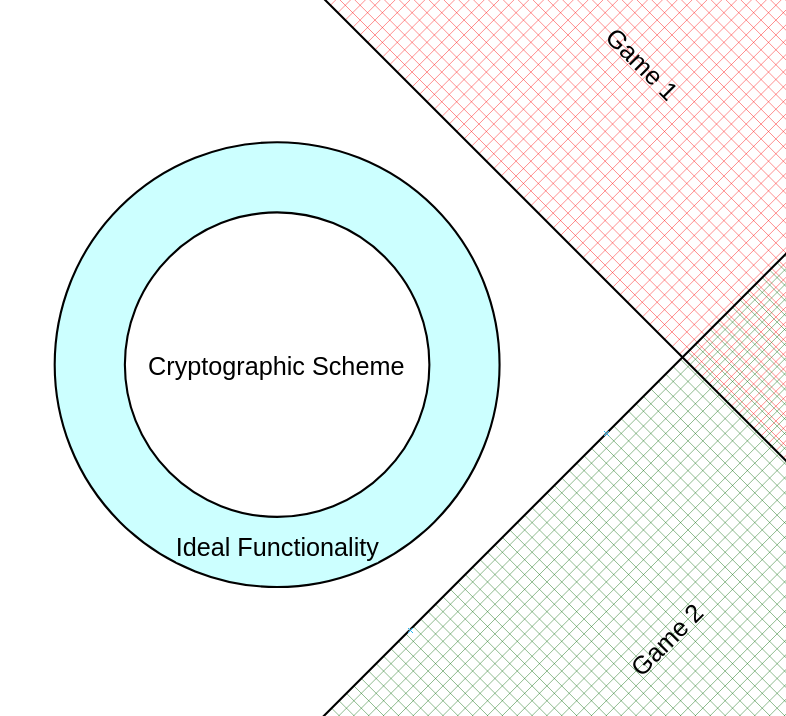
\includegraphics[width=10cm]{./01_body/images/simulation_vs_game_based_security.png}
\centering
\caption{Σχηματική αναπαράσταση Απόδειξης ασφάλειας μέσω παιχνιδιού και μέσω προσομοίωσης}
\label{fig:game_proof_vs_simulation_proof}
\end{figure}


\chapter{Ασφαλής Υπολογισμός Πολλών Μερών}
\label{chapter:SMPC}

Στην ενότητα αυτή θα γίνει μια εισαγωγή στον Ασφαλή Υπολογισμό Πολλών Μερών (Secure Multi Party Computation ή (SMPC)) και στη συνέχεια θα περιγραφούν και θα αναλυθούν ορισμένα βασικά πρωτόκολλα που χρησιμοποιούνται μέχρι και σήμερα. Σχετικά με την ανάλυση των πρωτοκόλλων, θα ξεκινήσουμε από τα πιο απλά και ιστορικά που είναι ασφαλή ενάντια σε παθητικούς αντιπάλους και θα συνεχίσουμε προς τα πιο σύνθετα και σύγχρονα που είναι ασφαλή ενάντια σε ενεργητικούς αντιπάλους. Δυστυχώς, παρότι σε κάποια πρωτόκολλα ίσως είναι προφανής η ιδιότητα της ασφάλεια τους για συγκεκριμένα μοντέλα αντιπάλων, η πλήρης τυποποιημένη απόδειξη της ασφάλειας αυτής για όλα τα πρωτόκολλα που θα αναλύσουμε θα χρειαζόταν τουλάχιστον κάποιες δεκάδες σελίδες σελίδες παραπάνω και θα ξέφευγε από τα πλαίσια της εργασίας αυτής. Ωστόσο, η μεθοδολογία που περιγράψαμε στο Κεφάλαιο \ref{chapter:security} καθώς και η παρατιθέμενη βιβλιογραφία δίνει ένα καλό εναρκτήριο σημείο για τον αναγνώστη που θέλει να εντρυφήσει στις αποδείξεις αυτές. Τα πρωτόκολλα που θα περιγράψουμε στο κεφάλαιο αυτό είναι τα Μπερδεμένα Κυκλώματα Yao, το BGW, το GMW και το SPDZ. Τα πρώτα τρία πρωτόκολλα υποστηρίζονται από τη βιβλιοθήκη ABY που χρησιμοποιούμε στο υλοποιητικό κομμάτι αυτής της εργασίας που βρίσκεται στο Κεφάλαιο \ref{chapter:implementation}. Είναι και τα τρία ασφαλή ενάντια σε παθητικούς αντιπάλους. Το τελευταίο πρωτόκολλο είναι ένα από τα πιο σύγχρονα και επιτυχημένα πρωτόκολλα που έχουν προταθεί στη βιβλιογραφία και παρότι δε σχετίζεται με την υλοποίηση επιλέξαμε να το αναλύσουμε για να υπάρχει σφαιρικότερη κάλυψη της βιβλιογραφίας, αφού είναι ασφαλές ενάντια σε ενεργητικούς αντιπάλους.

Στο Κεφάλαιο \ref{chapter:intro} κάναμε μια πολύ μικρή εισαγωγή στον κλάδο SMPC. Τα SMPC είναι διαδραστικά πρωτόκολλα στα οποία συμμετέχουν δύο ή περισσότεροι συμμετέχοντες, οι οποίοι διαθέτουν καμία, μία ή περισσότερες ιδιωτικές εισόδους. Η συνάρτηση που πρέπει να αποτιμηθεί για τις εισόδους αυτές, πρέπει να είναι από πριν γνωστή στους συμμετέχοντες, ώστε σε πρωτόκολλα που το υποστηρίζουν να μπορούν να επαληθεύσουν αν αυτή που πρόκειται να αποτιμηθεί είναι η προσυμφωνηθήσα συνάρτηση. Σχετικά με την ασφάλεια του Υπολογισμού Πολλών Μερών είναι σημαντικό να αναφέρουμε ότι τα πρωτόκολλα SMPC μεριμνούν αποκλειστικά και μόνο για την ασφαλή αποτίμηση του υπολογισμού. Αυτό σημαίνει ότι το αποτέλεσμα της αποτίμησης του υπολογισμού μπορεί να αποκαλύπτει σημαντικές πληροφορίες για την είσοδο κάποιου άλλου συμμετέχον, όπως για παράδειγμα στην περίπτωση μιας πύλης AND με δύο εισόδους όπου ελέγχονται από δύο συμμετέχοντες αντίστοιχα. Ας αναλογιστούμε το παράδειγμα της Ασφάλειας μέσω Προσομοίωσης, η οποία χρησιμοποιείται κατά κόρον στον κλάδο του SMPC. Στην περίπτωση αυτή, ένα πρωτόκολλο SMPC που έχει αποδειχθεί ασφαλές με αυτήν τη μέθοδο μας διασφαλίζει ότι οποιοσδήποτε αντίπαλος που ελέγχει κάποιους διεφθαρμένους συμμετέχοντες που συμμετέχουν στο πρωτόκολλο για την αποτίμηση του υπολογισμού δε μαθαίνει καμία πληροφορία παραπάνω από τη διαδικασία εκτέλεσης του πρωτοκόλλου, σε σχέση με την πληροφορία που θα μάθαινε αν συμμετείχε σε ένα πρωτόκολλο ιδανικού κόσμου. Προφανώς, ο αριθμός των διεφθαρμένων συμμετεχόντων που ελέγχονται από τον αντίπαλο, η υπολογιστική ισχύς του αντιπάλου καθώς και ο τρόπος διαφθοράς των συμμετεχόντων εξαρτάται από το μοντέλο αντιπάλου που έχουμε επιλέξει. Είναι αντιληπτό ότι τη γνώση που θα αποκτούσε ένας αντίπαλος στην περίπτωση μιας πύλης AND θα την αποκτούσε σε οποιοδήποτε, ιδανικό ή μη, πρωτόκολλο αποτίμησης της.

Στην ενότητα αυτή βασικές βιβλιογραφικές πηγές αποτέλεσαν τα βιβλία \cite{10.1561/3300000019} και \cite{cramer2015secure}. Επίσης, χρήσιμες εργασίες εισαγωγής και σύνοψης του κλάδου, αποτελούν οι \cite{cryptoeprint:2020/300} και  \cite{zhao2019secure}. Στην συνέχεια θα αναλύσουμε τα βασικά χαρακτηριστικά με βάση τα οποία μπορούμε να κατηγοριοποιήσουμε τα πρωτόκολλα SMPC.

\section{Κατηγορίες πρωτοκόλλων ως προς το μοντέλο αναπαράσταση του υπολογισμού}

Οποιοδήποτε πρωτόκολλο SMPC, για να εκτελέσει τον υπολογισμό μιας συνάρτησης $f$, χρειάζεται να λάβει την συνάρτηση σε μια συγκεκριμένη μορφή που εξαρτάται από το τύπο του πρωτοκόλλου. Δηλαδή, αν θέλουμε να χρησιμοποιήσουμε το πρωτόκολλο αυτό καλούμαστε να αναπαραστήσουμε την $f$ στο κατάλληλο υπολογιστικό μοντέλο για το οποίο έχει φτιαχτεί το πρωτόκολλο. Αυτό συμβαίνει, με οποιαδήποτε μηχανή υπολογισμού, σε έναν Επεξεργαστή (CPU) ή σε μια Εικονική Μηχανή για παράδειγμα χρειάζεται να αναπαραστήσουμε την $f$ στην κατάλληλη συμβολική γλώσσα ενώ σε μια Μηχανή Turing χρειάζεται να την αναπαραστήσουμε με την κατάλληλη αλγεβρική δομή. Στην περίπτωση των πρωτοκόλλων SMPC οι κύριες κατηγορίες που τα διακρίνουμε ως προς την αναπαράσταση της $f$ είναι οι παρακάτω :

\begin{definition}
\textbf{Κύρια Υπολογιστικά Μοντέλα των SMPC πρωτοκόλλων :}
\begin{itemize}
    \item Αναπαράσταση ως Boolean δίκτυο/κύκλωμα Συνδυαστικής Λογικής
    \item Αναπαράσταση ως Αριθμητικό δίκτυο/κύκλωμα, ένα παράδειγμα τέτοιου δικτύου δίνεται στο Σχήμα  \ref{fig:arithmetic-circuit}
    \item Πιο σύνθετες αναπαραστάσεις, όπως ως Μηχανή Turing ή RAM (Random Access Machine)
\end{itemize}
\end{definition}

\begin{figure}
    \begin{center}
        \usetikzlibrary {graphs}
        \tikz
        \graph [nodes={draw, circle}] {
                {x, y} -> {+} -> {*} -> w,
            y -> {*}
        };
        \caption{Παράδειγμα αριθμητικού δικτύου}
        \label{fig:arithmetic-circuit}
    \end{center}
\end{figure}

Στα πλαίσια αυτής της εργασίας θα αναφερθούμε μόνο σε πρωτόκολλα που ανήκουν στις πρώτες δύο κατηγορίες. Τα πρωτόκολλα που ανήκουν στην τελευταία κατηγορία αποτελούν ιδιαίτερα ενεργό ερευνητικό κλάδο την τελευταία δεκαετία με αρκετά σημαντικές εργασίες όπως οι \cite{cryptoeprint:2014/082} και \cite{goldwasser2013run}.

Προφανώς, οι παραπάνω κατηγορίες Boolean και Αριθμητικών δίκτυο σχετίζονται μεταξύ τους καθώς μπορούμε εύκολα να χρησιμοποιήσουμε ένα Αριθμητικό δίκτυο για τον υπολογισμό ενός Boolean κυκλώματος. Αν πάρουμε για παράδειγμα μια πύλη AND μπορούμε να τη μετατρέψουμε σε αριθμητική ως εξής :
%
\[
\begin{aligned}
    NAND(x, y)  &= AND(OR(x,y), OR(x,NOT(y)), OR(NOT(x),y)) =\\
                &= OR(x,y) + OR(x,NOT(y)) + OR(NOT(x),y) =\\
                &= x \cdot y + x \cdot NOT(y) + NOT(x) \cdot y =\\
                &= x \cdot y + x \cdot (1-y) + (1-x) \cdot y
\end{aligned}
\]
%
Στην συγκεκριμένη μαθηματική έκφραση κάνουμε διαχωρισμό μεταξύ των λογικών πυλών τις οποίες σημειώνουμε με τα ονόματα τους και των συμβόλων τις πρόσθεσης, της αφαίρεσης και του πολλαπλασιασμού οι οποίες αναφέρονται στο μαθηματικό δακτύλιο ή πεδίο στο οποίο ανήκουν τα στοιχεία $x,y$. Μπορούμε επίσης να χρησιμοποιήσουμε και ένα Boolean κύκλωμα για τον υπολογισμό ενός αριθμητικού δικτύου, χρησιμοποιώντας χρησιμοποιώντας, για παράδειγμα, έναν την αναπαράσταση ενός Αθροιστή (Adder) ή ενός Πολλαπλασιαστή (Multiplier) σε Boolean πύλες. Με παρόμοιο τρόπο λειτουργεί και η βιβλιοθήκη MPC-BLAS που υλοποιήσαμε και στην οποία θα αναφερθούμε στο Κεφάλαιο \ref{chapter:implementation}. Συνήθως βέβαια πρέπει να τονίσουμε πως οι μετατροπές από το έναν τρόπο υπολογισμού στον άλλο δεν είναι ιδιαίτερα αποδοτικές. Δηλαδή η χρήση ενός Boolean κυκλώματος για την εκτέλεση μιας πράξης πολλαπλασιασμού δεν ενδύκνειται, ωστόσο δεν έχουμε πάντα την επιλογή.

Σε αυτό το σημείο πρέπει να αναφερθεί πως ορισμένα πρωτόκολλα SMPC υποστηρίζουν μόνο πεπερασμένο υπολογισμό, δηλαδή πεπερασμένους σε χρόνο αλγορίθμους, και άρα δεν μπορεί να περιέχει άπειρους βρόγχους. Δηλαδή, απαιτείται να γίνει Ξετύλιγμα των βρόγχων (Loop unrolling) στην περίπτωση που υπάρχουν. Αυτό συνήθως συμβαίνει σε πρωτόκολλα στα οποία το κύκλωμα πρέπει να αρχικοποιηθεί (bootstrap) ολόκληρο πριν ξεκινήσει ο υπολογισμός. Στα πρωτόκολλα που θα εξετάσουμε δε συμβαίνει αυτό στην περίπτωση της ασφάλειας ενάντια σε παθητικούς αντιπάλους. Ωστόσο, είμαστε αντιμέτωποι με το εμπόδιο αυτό αν επιθυμήσουμε να μετατρέψουμε τα πρωτόκολλα αυτά σε ασφαλή ενάντια σε ενεργητικούς αντιπάλους μέσω κάποιων ειδικών τεχνικών που θα εξετάσουμε στη συνέχεια του κεφαλαίου.

\section{Κατηγορίες πρωτοκόλλων ως προς τις ιδιότητες ασφάλειας}

Όπως προαναφέραμε, το μοντέλο αναπαράστασης του υπολογισμού που χρησιμοποιεί ένα πρωτόκολλο είναι σύμφυτο με αυτό. Ένα ακόμα σύμφυτο χαρακτηριστικό ενός πρωτοκόλλου είναι η ασφάλεια του. Γενικότερα στα πρωτόκολλα SMPC διακρίνουμε τις παρακάτω κατηγορίες ασφάλειας πρωτοκόλλων :

\begin{itemize}
    \item Πρωτόκολλα ασφαλή ενάντια σε Παθητικούς Αντιπάλους
        \begin{itemize}
            \item Ασφαλή ενάντια σε διεφθαρμένη μειοψηφία
            \item Ασφαλή ενάντια σε διεφθαρμένη πλειοψηφία
        \end{itemize}
    \item Πρωτόκολλα ασφαλή ενάντια σε Ενεργητικούς Αντιπάλους
        \begin{itemize}
            \item Ασφαλή ενάντια σε διεφθαρμένη μειοψηφία
            \item Ασφαλή ενάντια σε διεφθαρμένη πλειοψηφία
        \end{itemize}
\end{itemize}

Προφανώς ένα πρωτόκολλο που είναι ασφαλές ενάντια σε ενεργητικούς αντιπάλους είναι ασφαλές και ενάντια σε παθητικούς. Το ίδιο ισχύει και στην περίπτωση της μειοψηφίας και πλειοψηφίας των διεφθαρμένων συμμετεχόντων. Στο Σχήμα \ref{fig:mp-sdpz-protocols} παραθέτουμε ,ενδεικτικά, των πίνακα υποστηριζόμενων πρωτοκόλλων και των μοντέλων ασφάλειας στα οποία είναι ασφαλή, της βιβλιοθήκης MP-SPDZ \cite{mp-spdz}. Η βιβλιοθήκη αυτή έχει ίσως την εκτενέστερη υποστήριξη πρωτοκόλλων στην βιβλιογραφία.

\begin{table}[h!]
    \centering
    \resizebox{\columnwidth}{!}{
        \begin{tabular}{|c|l|ll|ll|}
            \hline
            \multicolumn{1}{|l|}{}       &                                                                      & \multicolumn{2}{c|}{Αριθμητικό δίκτυο}                                    & \multicolumn{2}{c|}{Boolean κύκλωμα}                                 \\ \hline
            \multicolumn{1}{|l|}{}       & \diagbox{Μοντέλο Ασφάλειας}{Υπολογιστικό Μοντέλο} & \multicolumn{1}{l|}{$modp$ ή $GF(2^n)$}          & $mod2^n$               & \multicolumn{1}{l|}{Δυαδική Διαμοίραση Μυστικών} & Μπερδεμένα Δίκτυα \\ \hline
            \multirow{}{}{Ενεργητικός}   & Διεφθαρμένη Πλειοψηφία                                               & \multicolumn{1}{l|}{MASCOT / LowGear / HighGear} & SPDZ2k                 & \multicolumn{1}{l|}{Tiny / Tinier}               & BMR               \\ \cline{2-6}
            & Εμπιστή Πλειοψηφία                                                   & \multicolumn{1}{l|}{Shamir / Rep3 / PS / SY}     & Brain / Rep3 / PS / SY & \multicolumn{1}{l|}{Rep3 / CCD / PS}             & BMR               \\ \cline{2-6}
            & Έμπιστη Υπερ-πλειοψηφία                                              & \multicolumn{1}{l|}{Rep4}                        & Rep4                   & \multicolumn{1}{l|}{Rep4}                        & N/A               \\ \hline
            Συγκαλλημένος                       & Διεφθαρμένη Πλειοψηφία                                               & \multicolumn{1}{l|}{CowGear / ChaiGear}          & N/A                    & \multicolumn{1}{l|}{N/A}                         & N/A               \\ \hline
            \multirow{}{}{Παθητικός} & Διεφθαρμένη Πλειοψηφία                                               & \multicolumn{1}{l|}{Semi / Hemi / Temi / Soho}   & Semi2k                 & \multicolumn{1}{l|}{SemiBin}                     & Yao's GC / BMR    \\ \cline{2-6}
            & Έμπιστη Πλειοψηφία                                                   & \multicolumn{1}{l|}{Shamir / ATLAS / Rep3}       & Rep3                   & \multicolumn{1}{l|}{Rep3 / CCD}                  & BMR               \\ \cline{2-6}
            & Dealer                                                               & \multicolumn{1}{l|}{Dealer}                      & Dealer                 & \multicolumn{1}{l|}{Dealer}                      & N/A               \\ \hline
        \end{tabular}
    }
    \caption{Πίνακας υποστηριζόμενων πρωτοκόλλων της βιβλιοθήκης MP-SPDZ \cite{mp-spdz}. Ο παρόν είναι εμπνευσμένος από έναν παρόμοιο, αλλά δυσανάγνωστο, πίνακα που υπάρχει στα εγχειρίδια χρήσης της.}
    \label{fig:mp-sdpz-protocols}
\end{table}

\section{Ασφαλής Υπολογισμός Πολλών Μερών ενάντια σε Παθητικούς Αντιπάλους}

Στη ενότητα αυτή θα εξετάσουμε τρία πρωτόκολλα ιστορικής σημασίας τα οποία χρησιμοποιούνται μέχρι και σήμερα λόγω της ευκολίας υλοποίησης τους και της απόδοσης τους. Τα πρωτόκολλα αυτά είναι τα Μπερδεμένα Δίκτυα Yao, το BGW και το GMW.

\subsection{Πρωτόκολλο Μπερδεμένων Δικτύων Yao (Yao's Garbled Circuits Protocol)}
\label{section:yaos-gc}

Το πρωτόκολλο αυτό όπως αναφέραμε και στην Ενότητα \ref{chapter:intro} προτάθηκε από τον Yao το 1986 στις εργασίες \cite{4568207} \cite{4568388}. Πιο συγκεκριμένα, προτάθηκε ως πρωτόκολλο επίλυσης του Προβλήματος των Εκατομμυριούχων, δηλαδή για την περίπτωση των δύο συμμετεχόντων (2PC). Το συγκεκριμένο πρωτόκολλο απαιτεί την μετατροπή του αλγορίθμου σε μια Boolean συνάρτηση ή αντίστοιχα σε ένα Boolean κύκλωμα Συνδυαστικής Λογικής. Παρακάτω, θα αναλύσουμε την περίπτωση των δύο συμμετεχόντων για μια αυθαίρετη Boolean συνάρτηση και μετά θα αναφερθούμε στο πως μπορεί να επιταχυνθεί ο υπολογισμός με τη χρήση Boolean κυκλώματος. Το πρωτόκολλο αυτό μπορεί να αποδειχθεί ότι είναι ασφαλές απέναντι σε Παθητικούς Αντιπάλους.

\subsubsection{Υπολογισμός με χρήση του Πίνακα Αναζήτησης της συνάρτησης $f$}

Έστω δύο συμμετέχοντες $P_1$ και $P_2$ που θέλουν να εκτελέσουν μια Boolean συνάρτηση $\mathbf{out} = f(\mathbf{x}, \mathbf{y})$ με $x$ και $y$ τα διανύσματα των εισόδων των $P_1$ και $P_2$ αντίστοιχα. Έστω επίσης $x_i^j$, το $i$-οστο bit του διανύσματος $x$ για την τιμή $j$ του bit αυτού.  Γνωρίζουμε πως μια Boolean συνάρτηση μπορεί να περιγραφεί πλήρως από τον Πίνακα Αναζήτησης της (Look-up table). Το πρωτόκολλο αυτό απαιτεί κάποιον συμμετέχον να κάνει την προετοιμασία (bootstraping) ο οποίος πρέπει να γνωρίζει τον πλήρη Πίνακα Αναζήτησης της συνάρτησης $f$. Ας υποθέσουμε ότι ο $P_1$ εκτελεί αυτή τη διαδικασία. Για μια από τις $2 \cdot (\abs{\mathbf{x}} + \abs{\mathbf{y}})$ γραμμές του πίνακα ο $P_1$ κρυπτογραφεί την αντίστοιχη έξοδο της συνάρτησης με $ \abs{\mathbf{x}} + \abs{\mathbf{y}}$ διαφορετικά και ομοιόμορφα τυχαία επιλεγμένα κλειδιά χρησιμοποιώντας ένα συμμετρικό κρυπτογραφικό σχήμα με τον εξής τρόπο. Σε κάθε bit εισόδου του πίνακα αντιστοιχεί και ένα ζεύγος κλειδιών, ένα για κάθε τιμή που μπορεί να πάρει, αυτά τα συμβολίζουμε ως $k_{x_i^j}$. Δηλαδή αν $\abs{x}=2$ και $\abs{y}=3$ τότε η έξοδος $\mathbf{out}$ για την ανάθεση τιμών $x=01$ και $y=101$ θα κρυπτογραφηθεί ως $Enc_{k_{x_1^0}, k_{x_0^1}, k_{y_2^1}, k_{y_1^0}, k_{y_0^1}}(\mathbf{out})$. Ένα παράδειγμα της μορφής του πίνακα αυτού βρίσκεται στο Σχήμα \ref{fig:yaos-gc-global-truth-table}. Ο $P_1$ αφού έχει ολοκληρώσει τη δημιουργία του κρυπτογραφημένου πίνακα αληθείας, εφαρμόζει ομοιόμορφα τυχαίες μεταθέσεις στις γραμμές του και τον αποστέλλει ολόκληρο στον $P_2$. Οι τυχαίες μεταθέσεις εφαρμόζονται στον πίνακα διότι αν ήταν γνωστή η διάταξη των γραμμών του από τον $P_2$ τότε αυτός αφού θα λάμβανε τα κατάλληλα κλειδία που αντιστοιχούν στην ιδιωτική του είσοδο θα μπορούσε βλέποντας την γραμμή που αντιστοιχεί στα κλειδιά που έχει λάβει να καταλάβει ποια είναι η είσοδος του $P_1$. Ωστόσο, η μετάθεση των γραμμών δημιουργεί ένα άλλο πρόβλημα. Ο $P_2$ θα πρέπει να προσπαθήσει να αποκρυπτογραφήσει κάθε γραμμή του πίνακα προκειμένου να βρει την σωστή στη χειρότερη περίπτωση ενώ κατά μέσο όρο θα πρέπει να προσπαθήσει να αποκρυπτογραφήσει τις μισές γραμμές του πίνακα. Μια γνωστή αποδοτική τεχνική επίλυσης του προβλήματος αυτού ονομάζεται Point-and-Permute \cite{10.1145/100216.100287}, στην οποία θεωρούμε το τελευταίο bit του κάθε κλειδιού ως ένα από τα bit του δείκτη που δείχνει που θα τοποθετηθεί η γραμμή αυτή κατά την μετάθεση. Δηλαδή αν στο παραπάνω παράδειγμα τα τελευταία bit των κλειδιών έχουν τις εξής τιμές :
%
\begin{align*}
    \text{Τελευταίο bit κλειδιού : }k_{x_1^0} = 1, k_{x_0^1} = 0, k_{y_2^1} = 1, k_{y_1^0} = 1, k_{y_0^1} = 0
\end{align*}
%
τότε η γραμμή αυτή θα αποθηκευτεί στην θέση $10110=22$ του πίνακα. Εφόσον έχουμε υποθέσει ότι τα κλειδιά είναι τυχαία επιλεγμένα η μέθοδος αυτή δεν επηρεάζει την ασφάλεια του πρωτοκόλλου. Ο $P_1$ αποστέλλει επίσης στον $P_2$, τα κατάλληλα κλειδιά κρυπτογράφησης $k_{x_i^j}$ για τις τιμές του διανύσματος εισόδου $\mathbf{x}$ που έχει επιλέξει. Δηλαδή στο προηγούμενο παράδειγμα θα στείλει τα κλειδιά $k_{x_1^0}$, $k_{x_0^1}$. Στην συνέχεια αποστέλλει στον $P_2$ τα κλειδιά που αντιστοιχούν στις τιμές του διανύσματος εισόδου $\mathbf{y}$, μέσω $|y|/(2 \cdot |y|)$ Ανυποψίαστης Μεταφοράς. Τέλος ο $P_2$ αφού έχει αποκτήσει όλα τα απαραίτητα κλειδιά για την αποκρυπτογράφηση της γραμμής του Πίνακα Αναζήτησης της $f$ που αντιστοιχεί στο $f(\mathbf{x}, \mathbf{y})$, την αποκρυπτογραφεί, βλέπει το αποτέλεσμα $\mathbf{out}$ και στην συνέχεια το στέλνει στον $P_1$.

\begin{figure}
    \centering
\[
    \begin{pmatrix}
        f(\mathbf{x}=00, \mathbf{y}=000)\\
        f(\mathbf{x}=00, \mathbf{y}=001)\\
        f(\mathbf{x}=00, \mathbf{y}=010)\\
        f(\mathbf{x}=00, \mathbf{y}=011)\\
        \vdots\\
        f(\mathbf{x}=11, \mathbf{y}=110)\\
        f(\mathbf{x}=11, \mathbf{y}=111)\\
    \end{pmatrix}
    \rightarrow
    \begin{pmatrix}
        Enc_{k_{x_1^0}, k_{x_0^0}, k_{y_2^0}, k_{y_1^0}, k_{y_0^0}}(f(\mathbf{x}=00, \mathbf{y}=000))\\
        Enc_{k_{x_1^0}, k_{x_0^0}, k_{y_2^0}, k_{y_1^0}, k_{y_0^1}}(f(\mathbf{x}=00, \mathbf{y}=001))\\
        Enc_{k_{x_1^0}, k_{x_0^0}, k_{y_2^0}, k_{y_1^1}, k_{y_0^0}}(f(\mathbf{x}=00, \mathbf{y}=010))\\
        Enc_{k_{x_1^0}, k_{x_0^0}, k_{y_2^0}, k_{y_1^1}, k_{y_0^1}}(f(\mathbf{x}=00, \mathbf{y}=011))\\
        \vdots\\
        Enc_{k_{x_1^1}, k_{x_0^1}, k_{y_2^1}, k_{y_1^1}, k_{y_0^0}}(f(\mathbf{x}=11, \mathbf{y}=110))\\
        Enc_{k_{x_1^1}, k_{x_0^1}, k_{y_2^1}, k_{y_1^1}, k_{y_0^1}}(f(\mathbf{x}=11, \mathbf{y}=111))\\
    \end{pmatrix}
\]
    \caption[Παράδειγμα της διαδικασίας κρυπτογράφησης του πίνακα αληθείας της συνάρτησης $f$ σε έναν νέο πίνακα αληθείας με το Πρωτόκολλο Μπερδεμένων Δικτύων Yao.]{Παράδειγμα της διαδικασίας κρυπτογράφησης του πίνακα αληθείας της συνάρτησης $f$ σε έναν νέο πίνακα αληθείας με το Πρωτόκολλο Μπερδεμένων Δικτύων Yao. Ο πίνακας αυτός διαφέρει από τον πραγματικό αφού στον πραγματικό οι γραμμές υπόκεινται σε μετάθεση σύμφωνα με τη τεχνική Point-and-Permute.}
    \label{fig:yaos-gc-global-truth-table}
\end{figure}

\subsubsection{Υπολογισμός με χρήση του Boolean Κυκλώματος της $f$}

Είναι προφανές ότι η παραπάνω μέθοδος δεν μπορεί να κλιμακωθεί σωστά αφού το μέγεθος του Πίνακα Αναζήτησης της $f$ αυξάνεται εκθετικά με το μέγεθος των εισόδων. Μια ιδέα για την επιτάχυνση του υπολογισμού της $f$ από ένα Μπερδεμένο Δίκτυο Yao είναι να την εκφράσουμε ως ένα Boolean Δίκτυο. Από την προσέγγιση αυτή προκύπτει ουσιαστικά και το όνομα αυτού του πρωτοκόλλου. Παρακάτω θα επανεξετάσουμε την αποτίμηση μιας συνάρτησης $f$ από τους δύο συμμετέχοντες $P_1$, $P_2$.

Ο $P_1$ όπως και προηγουμένως είναι αυτός που αναλαμβάνει να αρχικοποιήσει το πρωτόκολλο. Στην προκείμενη περίπτωση να κατασκευάσει το Μπερδεμένο Κύκλωμα. Το κύκλωμα αυτό προκύπτει από το Boolean κύκλωμα της $f$ το οποίο και πρέπει να δημιουργήσει ο $P_1$. Για να το μετατρέψει στο αντίστοιχο Μπερδεμένο Κύκλωμα, δημιουργεί ένα ζεύγος κλειδιών για κάθε καλώδιο του κυκλώματος καθώς και δύο τυχαία συμπληρωματικά bit δεικτοδότησης (παραπλήσια με την τεχνική point-and-permute) για κάθε ζεύγος κλειδιών. Έτσι σε κάθε ζεύγος κλειδιών ενός καλωδίου $i$ αντιστοιχεί η εξής πλειάδα, την οποία ονομάζουμε \textbf{Ετικέτα του καλωδίου} :
%
\[
    w_i^b = (k_i^b \in \bin^\secparam, p_i^b \in \bin) \text{ όπου } p_i^b = 1-p_i^{1-b}
\]
%
Στη συνέχεια ο $P_1$ διατρέχει με το κύκλωμα σύμφωνα με την τοπολογική του διάταξη. Για μια αυθαίρετη πύλη $g_k$ του κυκλώματος, όπως αυτή του Σχήματος \ref{fig:yaos-gc-gate} ανάλογα με το αν είναι πύλη εισόδου, ενδιάμεση ή εξόδου εκτελεί ένα από τα βήματα που εξετάζουμε στη συνέχεια. Η διαφοροποίηση της παραλλαγής αυτής του πρωτοκόλλου σε σχέση με την προηγούμενη παραλλαγή που εξετάσαμε είναι πως για κάθε πύλη του κυκλώματος θα δημιουργήσουμε έναν πίνακα αληθείας. Για να διαχωρίσουμε τους δύο πίνακες θα ονομάσουμε τον πίνακα της προηγούμενης παραλλαγής ολικό πίνακα αληθείας και τον πίνακα αυτής της παραλλαγής τοπικό πίνακα αληθείας. Οι δύο πίνακες αυτοί έχουν μια βασική διαφορά στην κατασκευή τους. Στον τελευταίο η έξοδος κάθε γραμμής είναι η πραγματική έξοδος του κυκλώματος, ενώ στον πρώτο η έξοδος κάθε ενδιάμεσης πύλης είναι ένα μια ετικέτα που περιέχει το κλειδί κρυπτογράφησης που χρησιμοποιείται στην κρυπτογράφηση των γραμμών των πινάκων που λαμβάνουν ως είσοδο την έξοδο αυτή και τα αντίστοιχα bit δεικτοδότησης. Στα σημείο αυτό, για χάριν απλότητας, υποθέτουμε ότι όλες οι πύλες του κυκλώματος διαθέτουν δύο bit εισόδου και ένα bit εξόδου. Προφανώς, ο αλγόριθμος μπορεί πολύ εύκολα να επεκταθεί και για αυθαίρετο αριθμό bit εισόδου και εξόδου. Εναλλακτικά, κατά την αρχικοποίηση του κυκλώματος ο $P_1$ μπορεί πολύ εύκολα μια πύλη αυτού του είδους να αντικατασταθεί με ένα ισοδύναμο συνδυασμό πυλών που αποτελείται μόνο από πύλες με δύο bit εισόδου και ένα bit εξόδου. Τα βήματα που ακολουθεί ο $P_1$ είναι τα εξής :

\begin{itemize}
    \item \textbf{Οποιαδήποτε πύλη} : Στην περίπτωση αυτή, ο $P_1$, για κάθε μία από τις $2^2$ πιθανές (πραγματικές) εισόδους $v_i$, $v_j \in \bin$ της πύλης πρέπει να δημιουργήσει μια γραμμή στον τοπικό πίνακα. Αν θεωρήσουμε $e_{v_i, v_j}$ τη τιμή εξόδου της γραμμής $v_iv_j$ τότε αυτή δημιουργείται ως εξής και τοποθετείται στη θέση $p_i^{v_i}p_j^{v_j}$:
    %
    \[
        e_{v_i, v_j} = Enc_{k_i^{v_i}, k_j^{v_j}, k}(w_k^{g_l(v_a, v_b)})
    \]
    %
    Ένα παράδειγμα μετασχηματισμού του τοπικού πίνακα μιας πύλης φαίνεται στο Σχήμα \ref{fig:yaos-gc-local-truth-table}.
    \begin{figure}[h]
              \centering
              \[
                  \begin{pmatrix}
                      G_l(x=0, y=1)\\
                      G_l(x=0, y=0)\\
                      G_l(x=1, y=0)\\
                      G_l(x=1, y=1)\\
                  \end{pmatrix}
                  \rightarrow
                  \begin{pmatrix}
                      Enc_{k_i^{0}, k_j^{0}, i}(w_k^{g_l(x=0, y=0)})\\
                      Enc_{k_i^{0}, k_j^{1}, i}(w_k^{g_l(x=0, y=1)})\\
                      Enc_{k_i^{1}, k_j^{0}, i}(w_k^{g_l(x=1, y=0)})\\
                      Enc_{k_i^{1}, k_j^{1}, i}(w_k^{g_l(x=1, y=1)})\\
                  \end{pmatrix}
              \]
          \caption[Παράδειγμα της διαδικασίας κρυπτογράφησης του πίνακα αληθείας της συνάρτησης $f$ σε έναν νέο πίνακα αληθείας με το Πρωτόκολλο Μπερδεμένων Δικτύων Yao.]{Παράδειγμα της διαδικασίας κρυπτογράφησης του πίνακα αληθείας της συνάρτησης $f$ σε έναν νέο πίνακα αληθείας με το Πρωτόκολλο Μπερδεμένων Δικτύων Yao. Ο πίνακας αυτός διαφέρει από τον πραγματικό αφού στον πραγματικό οι γραμμές υπόκεινται σε μετάθεση σύμφωνα με τη τεχνική των bit δεικτοδότησης που αναλύσαμε.}
          \label{fig:yaos-gc-local-truth-table}
    \end{figure}
    \item \textbf{Καλώδια εξόδου} : Στην περίπτωση αυτή ακολουθείται ίδια διαδικασία με οποιοδήποτε άλλο καλώδιο μόνο που η τιμή που θα κρυπτογραφήσουμε θα πρέπει να είναι η έξοδος του καλωδίου και όχι κάποιο κρυπτογραφικό κλειδί που χρησιμοποιείται στην αποκρυπτογράφηση των εξόδων των πυλών που δέχονται το καλώδιο εξόδου ως είσοδο. Αν υποθέσουμε ότι η τιμή του καλωδίου εξόδου $w_i$ είναι η $v_i$ τότε τα καλώδια εξόδου δημιουργούνται ως εξής :
    \[
        e_v = Enc_{k_i^v_i, i}(v_i)
    \]
\end{itemize}

\begin{figure}
    \centering
    \begin{circuitikz}
        \draw
        (0,0) node[ieeestd and port](myand){}
        (myand.in 1) node[left]{$w_i^0, w_i^1$}
        (myand.in 2) node[left]{$w_j^0, w_j^1$}
        (myand.out) node[right]{$w_k^0, w_k^1$};
    \end{circuitikz}
    \caption{Παράδειγμα πύλης Μπερδεμένου Δικτύου Yao στην οποία φαίνονται οι δύο ετικέτες του κάθε καλωδίου μιας πύλης.}
    \label{fig:yaos-gc-gate}
\end{figure}

%It is more challenging to make this protocol secure against a malicious adversary that deviates from the protocol. One of the first solutions to make the protocol secure against malicious adversary is to use zero-knowledge proof to prevent malicious activities during the protocol.[11] For years, this approach was considered more as theoretical solution than a practical solution because of complexity overheads of it. But, it is shown that it is possible to use it with just a small overhead.[12] Another approach is using several GC for a circuit and verifying the correctness of a subset of them and then using the rest for the computation with the hope that if the garbler was malicious, it would be detected during the verification phase.[13] Another solution is to make the garbling scheme authenticated such that the evaluator can verify the garbled circuit.[14][15]

\subsection{Πρωτόκολλο Ben-Or, Goldwasser, Wigderson (BGW Protocol)}

Το πρωτόκολλο αυτό προτάθηκε από τους Ben-Or, Goldwasser, Wigderson στην εργασία \cite{BenOr1988CompletenessTF}. Απαιτεί την μοντελοποίηση της $f$ ως ένα Αριθμητικό Δίκτυο σε ένα πεπερασμένο πεδίο $\mathbb{F}$. Στην αρχική του μορφή βασίζεται στη Διαμοίραση Μυστικών Shamir και πιο συγκεκριμένα στις ομομορφικές ιδιότητες που παρουσιάζουν οι μετοχές του (για περισσότερες πληροφορίες σχετικά με τις ομομορφικές ιδιότητες μπορείτε να ανατρέξετε στο Κεφάλαιο \ref{chapter:cryptography} και στο Παράρτημα \ref{chapter:appendix}), ωστόσο μπορούν να χρησιμοποιηθούν και άλλες μέθοδοι διαμοίρασης μυστικών υπό την προϋπόθεση ότι παρουσιάζουν τις ίδιες ομομορφικές ιδιότητες. Όπως αναλύθηκε στο παράρτημα, το SSS είναι προσθετικά ομομορφικό από μόνο του, οπότε κύρια καινοτομία του πρωτοκόλλου BGW είναι η μετατροπή του SSS ώστε να μπορεί είναι και πολλαπλασιαστικά ομομορφικό. Παρακάτω, θα εξετάσουμε τις περιπτώσεις της ομομορφικής πρόσθεσης και πολλαπλασιασμού στην περίπτωση της μιας αριθμητικής πύλης και $n$ συμμετεχόντων και στην συνέχεια θα εξετάσουμε πως μπορούμε να γενικεύσουμε το πρωτόκολλο στην περίπτωση των περισσότερον πυλών. Το πρωτόκολλο αυτό μπορεί να αποδειχθεί ότι είναι ασφαλές ενάντια σε Παθητικούς Αντιπάλους που ελέγχουν τη μειοψηφία των συμμετεχόντων, δηλαδή με διεφθαρμένη μειοψηφία συμμετεχόντων.

Έστω ότι $n$ συμμετέχοντες όπου θέλουν να αποτιμήσουν μια αριθμητική συνάρτηση ή αντίστοιχα ένα αριθμητικό δίκτυο και ας υποθέσουμε όπως και στην Ενότητα \ref{section:yaos-gc}, ότι $out = f(x, y)$, όπου $x$, $y$, είναι οι είσοδοι της συνάρτησης και η καθεμία ελέγχεται από κάποιον συμμετέχον. Η αριθμητική συνάρτηση $f$ πρέπει να είναι γνωστή σε όλους τους συμμετέχοντες. Επίσης, ο κάθε συμμετέχον διαθέτει ένα σημείο $i \in \mathbb{F}$, το οποίο το γνωρίζουν όλοι οι συμμετέχοντες στο δίκτυο, το οποίο χάριν απλότητας ας υποθέσουμε ότι το $i$ είναι ο αύξων αριθμός του συμμετέχοντος και $i = 0, \ldots, n-1 \in \mathbb{F}$. Στην συνέχεια της ενότητας, ο συμβολισμός $i$ θα χρησιμοποιείται για να αναφερθούμε είτε στο σημείο του παίχτη $i$ είτε στον ίδιο τον παίχτη $i$. Στην συνέχεια ανάλογα με την πύλη του αριθμητικού κυκλώματος εκτελείται ένα μια από τις παρακάτω διαδικασίες :

\begin{itemize}
    \item \textbf{Καλώδιο Εισόδου} : Στην περίπτωση της εισόδου, ο συμμετέχον, ας τον ονομάσουμε $P$, που ελέγχει την είσοδο είσοδο, ας την ονομάσουμε $x$, διαμοιράζει μέσω $SSS(n,t)$ την τιμή της $x$, υπό τον περιορισμό ότι $2t + 1 < n$ (θα αιτιολογηθεί στην συνέχεια ο περιορισμός αυτός) και δίνει αντίστοιχες μετοχές $[x]_i$ σε κάθε άλλον συμμετέχον $i \in 0, 1, \ldots n$. Όπως γνωρίζουμε από το $SSS$, η μετοχή του παίχτη $i$ είναι ένα σημείο $(i, p_x(i))$, για την είσοδο $x$ και το $p_x$ είναι το πολυώνυμο $t$-οστού βαθμού που επέλεξε ο συμμετέχον $P$.
    \item \textbf{Πύλη Πρόσθεσης} : Στην περίπτωση αυτή, υποθέντωντας ότι έχουμε μια πύλη πρόσθεσης με δύο εισόδους, τότε κάθε συμμετέχον $i$ διαθέτει μια μετοχή $[x]_i$ και μια $[y]_i$ αντίστοιχα. Κάθε συμμετέχον μπορεί να εκτελέσει την πράξη $x+y$, απλώς αθροίζοντας τις τετμημένες των αντίστοιχων μετοχών, δηλαδή $[c]_i = [x]_i + [y]_i$. Το παραπάνω προκύπτει από την ιδιότητα της γραμμικότητας του $SSS$ που αναλύθηκε στο Κεφάλαιο \ref{chapter:cryptography}, αφού προκύπτει ότι $[c]_i = [x]_i + [y]_i = p_x(i) + p_y(i) = p_{x+y}(i) = [x + y]_i$. Η πράξη της πρόσθεσης δεν απαιτεί καμία αλληλεπίδραση μεταξύ των συμμετεχόντων αφού ο καθένας τους διαθέτει τις μετοχές $[x]_i$ και $[y]_i$.
    \item \textbf{Πύλη Πολλαπλασιασμού} :
        \begin{itemize}
            \item \textbf{Βαθμωτός πολλαπλασιασμός} : Παρόμοια με την πράξη της πρόσθεσης από την γραμμική ιδιότητα του $SSS$ προκύπτει ότι $[c]_i = b \cdot [x]_i = b \cdot p_x(i) = p_{b \cdot x}(i) = [b \cdot x_i ]$.
            \item \textbf{Πολλαπλασιασμός με μεταβλητή} : Κάθε συμμετέχον $i$ διαθέτει μια μετοχή $[x]_i$ και μια $[y]_i$ αντίστοιχα. Όπως και με τους υπόλοιπους τελεστές αρχικά ο κάθε συμμετέχον υπολογίζει την μετοχή $[c]_i = [x]_i \cdot [y]_i$. Γνωρίζουμε ότι $[c]_i = [x]_i \cdot [y]_i = p_x(i) \cdot p_y(i) = p_{x \cdot y}(i) (= p_c(i))= [x \cdot y]_i$. Όπως παρατηρούμε το πρόβλημα που προκύπτει στην πράξη του πολλαπλασιασμoύ είναι ότι ο πολλαπλασιασμός δύο πολυωνύμων $t$-οστού βαθμού, όπως στην προκείμενη περίπτωση των $p_x$ και $p_y$, μπορεί να μας δώσει ως αποτέλεσμα ένα πολυώνυμο μέχρι και $2t$-οστού βαθμού. Είναι απαραίτητο να κρατήσουμε σταθερό αυτό το κατώφλι $t$. Για να το επιτύχουμε αυτό αρχικά ο κάθε συμμετέχον εκτελεί τον πολλαπλασιασμό των μετοχών $[c]_i = [x]_i \cdot [y]_i$, όπως προαναφέραμε. Στο σημείο αυτό, εξετάζουμε την χειρότερη περίπτωση, δηλαδή ότι το $[c]_i$ έχει κατώφλι διαμοίρασης $2t$. Για να μειωθεί το κατώφλι σε $t$, ο κάθε συμμετέχον $i$ διαμοιράζει το $[c]_i$ με $SSS(n, t)$, ας υποθέσουμε ότι χρησιμοποιεί για αυτό ένα τυχαίο πολυώνυμο $p_{h_i}(x)$ όπου προφανώς $p_{h_i}(0)=[c]_i=p_c(i)$, και στην συνέχεια διαμοιράζει τις μετοχές που αντιστοιχούν στον καθένα από τους υπόλοιπους $n-1$ συμμετέχοντες. Δηλαδή, στον παίχτη $j$ ο παίχτης $i$ θα στείλει την τιμή $p_{h_i}(j)$. Έτσι, ο κάθε συμμετέχον $j$ διαθέτει τις μετοχές $p_{h_i}(j)$ για κάθε $i \in 1, 2, \ldots, n$. Στην συνέχεια κάθε συμμετέχον υπολογίζει την τελική του μετοχή ως εξής :
            
            \begin{equation}\label{eq:bgw1}
            p_h(j) = \sum_{i=1}^{2t+1}λ_i(x)p_{h_i}(j)
            \end{equation}
            
            όπου $λ_i$ είναι ο κατάλληλος συντελεστής που αναφέρεται στο παράρτημα και μπορεί να υπολογιστεί από κάθε συμμετέχοντα αφού είναι δημόσια γνωστό στους συμμετέχοντες ότι $α_i=i$. Επειδή, η ορθότητα της Σχέσης \ref{eq:bgw1} ίσως να μην είναι προφανής ας σταθούμε λίγο περισσότερο σε αυτήν. Η Σχέση \ref{eq:bgw1} μπορεί να αναπτυχθεί στην παρακάτω :
            \[
                 p_h(j) = \sum_{i=1}^{2t+1}λ_i(x)p_{h_i}(j) = λ_1p_{h_1}(j) + λ_2p_{h_2}(j) + \ldots + λ_n p_{h_n}(j)
            \]
            και ουσιαστικά το πολυώνυμο $p_h(x)$ του οποίου σημείο είναι το $p_h(j)$ είναι το παρακάτω : 
            \[
                p_h(x) = λ_1p_{h_1}(x) + λ_2p_{h_2}(x) + \ldots + λ_n p_{h_n}(x)
            \]
            Ισχύει ότι $deg(p_h(x))=t$ αφού είναι άθροισμα των πολυωνύμων $p_{h_i}$ για καθένα από τα οποία ισχύει $deg(p_{h_i} = t)$. Επίσης, μπορούμε να επαληθεύσουμε ότι $p_h(0)=p_c(0)$ αφού
            
            \begin{align}
                p_h(0) &= λ_1 p_{h_1}(0) + λ_2 p_{h_2}(0) + \ldots + λ_n p_{h_n}(0) \\
                &= λ_1 p_c(1) + λ_2 p_c(2) + \ldots + λ_n p_c(n) \\
                &= p_c(0)
            \end{align}
        \end{itemize}
    \item \textbf{Καλώδιο Εξόδου} : Στην περίπτωση αυτή το μόνο που έχουν να κάνουν οι συμμετέχοντες είναι να ανοίξουν τις μετοχές τους όπως περιγράφεται στο Πρωτόκολλο SSS, στο Κεφάλαιο \ref{chapter:cryptography}.
\end{itemize}

\subsubsection{Επιτάχυνση του πρωτοκόλλου με χρήση Πολλαπλασιαστικών Τριάδων Beaver (Beaver Triples)}
Στο πρωτόκολλο BGW, στην περίπτωση του πολλαπλασιασμού που έχει προκύψει από είσοδο, κάθε παίχτης πρέπει να εκτελέσει $SSS(n,t)$ και δηλαδή να διαμοιράσει $n$ μετοχές. Αυτό έχει πολυπλοκότητα επικοινωνίας $O(n^2)$. Μπορούμε να βελτιώσουμε την παραπάνω πολυπλοκότητα επικοινωνίας αν χωρίσουμε τον υπολογισμό σε δύο φάσεις, την \textbf{Φάση προεπεξεργασίας (Preprocessing phase)} και την \textbf{Online φάση}. Έτσι μπορούμε να επιτύχουμε βελτίωση της πολυπλοκότητας επικοινωνίας με τον εξής τρόπο. Η επιτάχυνση μπορεί να συμβεί με τον παρακάτω τρόπο.

Ας υποθέσουμε ότι $x$ και $y$ είναι οι είσοδοι της πολλαπλασιαστικής πύλης για τις οποίες κάθε συμμετέχον διαθέτει μετοχές $[x]$ και $[y]$ αντίστοιχα. Επίσης έστω οι τιμές $a, b \sample \mathbb{F}$, $c=a \cdot b$ και οι αντίστοιχες μετοχές $[a]$, $[b]$, $[c]$ τους. Τότε ο κάθε συμμετέχον μπορεί να υπολογίσει την πολλαπλασιαστική πύλη ακολουθώντας τα παρακάτω βήματα :

\begin{enumerate}
    \item Υπολογίζει τα $[x - a]$ και $[y - b]$ και ανακοινώνει δημόσια τις τιμές $d = x - a$ και $e = y - b$.
    \item Υπολογίζει το $de + d[b] + e[a] + [c] = [x \cdot y]$ αφού,
    \begin{align}
        xy &= (x - a + a)(y - a + a) \\
           &= (d + a)(d + b) \\
           &= de + db + ae + ab \\
           &= de + db + ae + c
    \end{align}
\end{enumerate}

Τέλος, να σημειώσουμε ότι ο διαχωρισμός του πρωτοκόλλου σε περισσότερες από μία φάσεις είναι κάτι πολύ σύνηθες στην περίπτωση των SMPC και FHE πρωτοκόλλων, που αποσκοπεί συνήθως στην εξοικονόμηση χρονικής ή χωρικής πολυπλοκότητας κάθε φάσης μέσω των προηγούμενων της. Μια τέτοια περίπτωση αποτελεί και το πρωτόκολλο SPDZ που θα εξετάσουμε σε επόμενη ενότητα.

\subsection{Πρωτόκολλο Goldreich, Micali, Wigderson (GMW Protocol)}

Το πρωτόκολλο αυτό προτάθηκε από τους Goldwasser, Micali, Wigderson στην εργασία \cite{goldreich2019play} το 1987. Απαιτεί την αναπαράσταση του υπολογισμού μιας συνάρτησης, $f$, ως Boolean κύκλωμα. Το πρωτόκολλο αυτό μοιάζει σε ένα βαθμό, με αυτό των Μπερδεμένων Δικτύων Yao, που περιγράψαμε προηγουμένως. Οι συμμετέχοντες έχουν ένα Boolean δίκτυο το οποίο αποτιμούν πύλη ανά πύλη (gate-by-gate) σύμφωνα με την τοπολογική τους σειρά. Ένα ακόμα κοινό χαρακτηριστικό, είναι ότι και το GMW χρησιμοποιεί OT για τον υπολογισμό ορισμένων Boolean πυλών. Σε αυτό το χαρακτηριστικό βασίζεται και η κύρια διαφορά των δύο πρωτοκόλλων. Το GMW απαιτεί ΟΤ μόνο στην περίπτωση της AND πύλης, ενώ οι πύλες NOT και XOR μπορούν να υπολογιστούν χωρίς OT. Το γεγονός αυτό κάνει το GMW κατά μέσο όρο πιο γρήγορο από τo Yao's GC. Μια ακόμα διαφορά τους είναι πως το πρωτόκολλο αυτό επιτρέπει την την συμμετοχή περισσότερων των δύο συμμετεχόντων στον υπολογισμό. Στην συνέχεια, θα επικεντρωθούμε στην περίπτωση των δύο συμμετεχόντων, ενώ θα αναφερθούμε λίγο αργότερα στο πως αυτή μπορεί να γενικευθεί σε για περισσότερους. Το πρωτόκολλο αυτό είναι ασφαλές ενάντια σε Παθητικούς αντιπάλους.

Θα εξετάσουμε την περίπτωση δύο συμμετεχόντων, $P_1$ και $P_2$, και μιας Boolean πύλης όπως αυτή του Σχήματος \ref{fig:gmw-gate} με δύο bit εισόδου και ένα bit εξόδου :
\begin{itemize}
    \item \textbf{Καλώδιο εισόδου} : Έστω πως ο συμμετέχον $P_1$ διαθέτει ένα ιδιωτικό bit εισόδου $x_i$ το οποίο αντιστοιχεί σε ένα καλώδιο $w_i$ του κυκλώματος. Έστω επίσης $s_i^j$, η μετοχή για το καλώδιο $w_i$ του παίχτη $j$. Για κάθε καλώδιο $i$ επιθυμούμε $s_i^j \oplus s_i^{j-1} = w_i$. Ο $P_1$ δημιουργεί τις μετοχές ως εξής :
    \begin{itemize}
        \item Στέλνει στον $P_2$ το $r_i \sample \bin$, η οποία είναι η μετοχή του $P_2$ για το καλώδιο $w_i$, δηλαδή $s_i^2 = r_i$
        \item Δημιουργεί τη δική του μετοχή του $w_i$ ως εξής : $s_i^1 = x_i \oplus r_i$
    \end{itemize}
    Ο σκοπός αυτού του τρόπου διαμοίρασης μετοχών είναι πως για κάθε καλώδιο η πραγματική του τιμή είναι η $w_i = s_i^1 \oplus s_i^2$. Ο λόγος για τον οποίο χρησιμοποιείται η πύλη XOR για τη διαμοίραση είναι πως
    \item \textbf{Πύλη NOT} : Έστω το καλώδιο εισόδου $w_k$ και το καλώδιο εξόδου $w_{k+1}$. Στην περίπτωση της Πύλης NOT, ένας από τους δύο συμμετέχοντες (όχι και οι δύο) τον οποίο πρέπει είτε να έχουν προαποφασίσει είτε εναλλακτικά να ρίξουν κάποιο τυχαίο νόμισμα μέσω Ανυποψίαστης Μεταφοράς, έστω ο $P_1$, το μόνο που έχει να κάνει είναι να αντιστρέψει το bit της μετοχής του, δηλαδή $s_{k+1}^1 = 1-s_k^1$
    \item \textbf{Πύλη XOR} : Έστω τα καλώδια εισόδου $w_k$, $w_{k+1}$ και το καλώδιο εξόδου $w_{k+2}$. Στην περίπτωση της Πύλης XOR, οι δύο συμμετέχοντες κάνουν XOR τις μετοχές που έχουν για κάθε μία από τις δύο εισόδους της πύλης. Δηλαδή $s_{k+2}^1 = s_{k}^1 \oplus s_{k+1}^1$ και $s_{k+2}^2 = s_k^2 \oplus s_{k+1}^2$
    \item \textbf{Πύλη AND}: Έστω τα καλώδια εισόδου $w_k$, $w_{k+1}$ και το καλώδιο εξόδου $w_{k+2}$. Στην περίπτωση της Πύλης AND, ο ένας από τους δύο συμμετέχοντες, έστω ο $P_1$ πρέπει να ετοιμάσει ένα 1-4 ΟΤ της παρακάτω συνάρτησης :
    \[
    S=S_{s_i^1, s_j^1}\left(s_i^2, s_j^2\right)=\left(s_i^1 \oplus s_i^2\right) \wedge\left(s_j^1 \oplus s_j^2\right)
    \]
    Αυτό το κάνει επιλέγοντας $r \sample \bin$ και στη συνέχεια δημιουργώντας τον παρακάτω πίνακα από τον οποία στέλνει την κατάλληλη γραμμή μέσω 1-4 OT ανάλογα με τη τιμή που έχουν οι μετοχές του $P_2$ :
    \[
    T_G=\left(\begin{array}{l}
                  r \oplus S(0,0) \\
                  r \oplus S(0,1) \\
                  r \oplus S(1,0) \\
                  r \oplus S(1,1)
    \end{array}\right)
    \]
    \item \textbf{Καλώδιο εξόδου} :
\end{itemize}

\begin{figure}
    \centering
    \begin{circuitikz}
        \draw
        (0,0) node[ieeestd and port](myand){}
        (myand.in 1) node[left]{$s_i^0, s_i^1$}
        (myand.in 2) node[left]{$s_j^0, s_i^1$}
        (myand.out) node[right]{$w_k^0, w_k^1$};
    \end{circuitikz}
    \caption{Παράδειγμα πύλης για το πρωτόκολλο GMW στη περίπτωση των δύο συμμετεχόντων}{Παράδειγμα πύλης για το πρωτόκολλο GMW στη περίπτωση των δύο συμμετεχόντων. Σε κάθε καλώδιο σημειώνονται οι δύο μετοχές που κρατάνε οι συμμετέχοντες για αυτό.}
    \label{fig:gmw-gate}
\end{figure}

\section{Ασφαλής Υπολογισμός Πολλών Μερών ενάντια σε Ενεργητικούς Αντιπάλους}

Η ενότητα αυτή δεν εμπίπτει πλήρως στους σκοπούς αυτής της εργασίας από την πρακτική σκοπιά αφού η βιβλιοθήκη MPC-BLAS δημιουργήσαμε και θα αναλύσουμε στο επόμενο κεφάλαιο είναι ασφαλής ενάντια σε Παθητικούς αντιπάλους. Ωστόσο, ο κλάδος αυτός πρόκειται για έναν από τους πιο ερευνητικά ενεργούς υποκλάδους του SMPC και θεωρούμε παράλειψη να μην αναφερθούμε σε αυτόν.  Γενικότερα, δημιουργία πρωτοκόλλων Ασφαλούς Υπολογισμού ασφαλή ενάντια σε Ενεργητικούς αντιπάλους δεν αποτελεί μια εύκολη υπόθεση. Για την επίτευξη αυτού του σκοπού έχουν αναπτυχθεί διάφορες τεχνικές τις οποίες θα εξετάσουμε συνοπτικά στην επόμενη ενότητα κια αμέσως μετά θα αναλύσουμε το πρωτόκολλο SPDZ που επιτυγχάνει το σκοπό αυτό.

\subsection{Τεχνικές Μετατροπής μετατροπής της ασφάλειας πρωτοκόλλων από Παθητική σε Ενεργητική}

Οι μεθοδολογίες που ακολουθούνται όταν θέλουμε να δημιουργήσουμε ένα πρωτόκολλο που να είναι ασφαλές ενάντια σε ενεργητικούς στη βιβλιογραφία χωρίζονται κυρίως σε δύο κύριες κατηγορίες. Στην πρώτη περίπτωση η αφετηρία μας είναι ένα πρωτόκολλο ασφαλές ενάντια σε παθητικούς αντιπάλους το οποίο στην συνέχεια μέσω τεχνικών προσπαθούμε να κάνουμε ασφαλές ενάντια σε ενεργητικούς αντιπάλους. Μερικές από τις τεχνικές που εφαρμόζονται είναι οι εξής :

\begin{itemize}
    \item Cut-and-Choose \cite{chaum1984blind}
    \item Μεταγλωττιστής GMW \cite{goldreich2019play}
    \item Αυθεντικοποιημένα Μπερδεμένα Δίκτυα \cite{wang2017authenticated}
\end{itemize}

Οι εναλλακτικές μέθοδος που μπορούμε να ακολουθήσουμε είναι να προσπαθήσουμε να δημιουργήσουμε ένα πρωτόκολλο ασφαλούς ενάντια σε ενεργητικούς αντιπάλους υποθέτοντας πως κάποια κρίσιμα κομμάτια του υλοποιούνται με κάποιο ιδανικό τρόπο, για παράδειγμα μέσω ενός έμπιστου τρίτου. Αυτός ο τρόπος, μας επιτρέπει να προχωρήσουμε τη διαδικασία σχεδίασης του πρωτοκόλλου. Στο τέλος της διαδικασίας προσπαθούμε να αντικαταστήσουμε τον έμπιστο τρίτο με κάποιο πρωτόκολλο ασφαλές ενάντια σε ενεργητικούς αντιπάλους ή παθητικούς αντιπάλους που να εκτελεί την διεργασία του. Αυτό τον τρόπο ακολουθεί και το πρωτόκολλο SPDZ που θα εξετάσουμε στη συνέχεια.

\subsection{Πρωτόκολλα Ασφαλή ενάντια σε Ενεργητικούς Αντιπάλους}

Η Online φάση του πρωτοκόλλου SPDZ όπως προαναφέραμε είναι ασφαλής ενάντια σε ενεργητικούς αντιπάλους που ελέγχουν διεφθαρμένη πλειοψηφία των συμμετεχόντων. Είναι σημαντικό να αναφέρουμε πως στη περίπτωση αυτή έχει αποδειχθεί ότι δεν μπορούν να υπάρξουν απόλυτα ασφαλή SMPC πρωτόκολλα, παρά μόνο υπολογιστικά ασφαλή πρωτόκολλα.

\subsection{Πρωτόκολλο SPDZ}

Το πρωτόκολλο SPDZ παρουσιάστηκε για πρώτη φορά το 2011 στην εργασία \cite{cryptoeprint:2011/535} και είναι άμεσα επηρεασμένο από την \cite{bendlin2011semi} που παρουσιάστηκε την ίδια χρονιά και υπήρξαν αρκετά κοινά μέλη στις δύο αυτές ερευνητικές ομάδες αλλά και από την \cite{ishai2007zero}. Το SPDZ απαιτεί την αναπαράσταση μια συνάρτησης $f$ που θέλουν να αποτιμήσουν οι συμμετέχοντες ως αριθμητικό δίκτυο. Το πρωτόκολλο, χωρίζεται σε δύο φάσεις, αυτή της Προεπεξεργασίας ή Offline(Preprocessing ή Offline phase) και την Online φάση (Online phase). Η πρώτη είναι ασφαλής ενάντια σε παθητικούς αντιπάλους ενώ η δεύτερη είναι ασφαλής ενάντια σε ενεργητικούς αντιπάλους. Δυστυχώς, δεν μπορούμε να καλύψουμε λεπτομερώς τη φάση προεπεξεργασίας διότι βασίζεται στην Κάπως Ομομορφική Κρυπτογραφία. Από τότε που προτάθηκε το SPDZ, έχουν υπάρξει διάφορες προτάσεις/βελτιώσεις του στη βιβλιογραφία οι οποίες κυρίως βελτιώνουν το κομμάτι της Προεπεξεργασίας, μερικές από αυτές είναι οι MASCOT. Σήμερα, με το όνομα SPDZ αναφερόμαστε γενικότερα στην κλάση των πρωτοκόλλων που βασίζονται στην εργασία \cite{cryptoeprint:2011/535}. Στην παράγραφο αυτή θα αναλύσουμε το πρωτόκολλο που προτάθηκε στην εργασία αυτή. Πριν ξεκινήσουμε με την ανάλυση του πρωτοκόλλου πρέπει πρώτα να σταθούμε στη σημειογραφία που χρησιμοποιείται σε αυτό.

\subsubsection{Σημειογραφία πρωτοκόλλου SPDZ}

Στα πλαίσια του πρωτοκόλλου αυτού όταν αναφερόμαστε σε Διαμοίραση Μυστικών εννοούμε Προσθετική Διαμοίραση Μυστικών. Το εργαλείο αυτό βρίσκεται στη καρδιά του SPDZ. Παρότι δεν το έχουμε ορίσει μέχρι στιγμής στην εργασία αυτή, λειτουργεί πολύ απλά. Κάθε μετοχή αποτελεί μια τιμή όπου το άθροισμα όλων των μετοχών αποκαλύπτουν το μυστικό της διαμοίρασης, δηλαδή είναι μια διαμοίραση με κατώφλι $n-n$, αν υποθέσουμε ότι έχουμε $n$ συμμετέχοντες. Υποθέτοντας ότι έχουμε $n$ συμμετέχοντες στο πρωτόκολλο, τότε κάθε τιμή ενός καλωδίου $x$ είναι διαμοιρασμένη σε όλους τους παίχτες. Συνολικά η τιμή $x$ περιγράφεται από την παρακάτω πλειάδα
\begin{equation}
\label{def:spdz-secret}
[ x ] = (δ, x^{1}, \ldots, x^{n}, m^{1} = γ_Δ(x^1), \ldots, m^{n} = γ_Δ(x^n), Δ^{1}, \ldots, Δ^{n})
\end{equation}
όπου ισχύουν οι εξής ιδιότητες :
\begin{equation}
    \label{def:spdz-secret-properties}
x=\sum_{i=1}^n x^{i}, x \cdot Δ + δ=(\sum_{i=1}^n m^{i}), \Delta=\sum_{i=1}^n \Delta^{i}
\end{equation}
Τον ρόλο της μεταβλητής $δ$ θα τον δούμε στην συνέχεια, η τιμή της στην αρχή του πρωτοκόλλου συνήθως είναι 0. Ο τιμές $x^i$ είναι οι προσθετικές μετοχές της $x$, οι τιμές $m_i$ είναι η προσθετικές μετοχή του σχήματος MAC και οι τιμές $Δ_i$ είναι οι προσθετικές μετοχές του σχήματος MAC. Το σχήμα MAC στην συγκεκριμένη περίπτωση, δεν σχετίζεται με τα σχήματα MAC που βασίζονται σε συμμετρικά κρυπτογραφικά σχήματα. Ορίζεται ως εξής :
\[
    m = \operatorname{MAC}_k(x) = γ_k(x) = k \cdot x \mod p \text{ , όπου $p$ πρώτος με το κατάλληλο μέγεθος.}
\]
Δηλαδή, από την Σχέση \ref{def:spdz-secret}, για κάθε καλώδιο, έστω $x$, του κυκλώματος ο κάθε συμμετέχον $P_i$ έχει στην κατοχή του την εξής πλειάδα :
\[
    [x]_i = (x^i, γ_Δ(x^i), Δ^i) \text{ για τα οποία ισχύει : } m_i = γ_Δ(x_i) = Δ_i \cdot x_i
\]
Στο σημείο αυτό να αναφέρουμε πως οι μετοχές για την τιμή $Δ$ δεν μεταβάλλονται από μετοχή σε μετοχή. Τις αναφέραμε για μεγαλύτερη πληρότητα της περιγραφής της μετοχής. Οι τιμές αυτές χρησιμοποιούνται μόνο όταν είναι να αποτιμηθούν οι έξοδοι του πρωτοκόλλου, οπότε θα τις παραλείπουμε στην περιγραφή μιας μετοχής και θα επανέλθουμε σε αυτές όταν θα αναλύσουμε αυτό το στάδιο του πρωτοκόλλου.

Στην περίπτωση πρόσθεσης μιας σταθεράς, έστω $ε$, σε μια μετοχή, έστω $[x]$, τότε αυτή εκτελείται ως εξής :
\[
    [x]' = ε+[x] = [ε + x] = (δ-ε, x^1+ε, x^2, \ldots, x^n, γ_Δ(x^1), γ_Δ(x^2), \ldots, γ_Δ(x^n))
\]
Παρατηρούμε ότι στην περίπτωση αυτή διατηρούνται οι ιδιότητες της Σχέσης \ref{def:spdz-secret-properties}, αφού :
\begin{equation}
    \begin{gathered}
    x'=\sum_{i=1}^n x^{i} + ε = x+ε\\
    x' \cdot Δ = (x'+ ε + δ) \cdot Δ = (x + ε - ε) \cdot Δ = x \cdot Δ\\
    \end{gathered}
\end{equation}
Παρατηρούμε επίσης ότι μόνο ένας συμμετέχον, επιλέξαμε αυθαίρετα τον $P_1$ θα προσθέσει την σταθερά στην μετοχή του, δηλαδή την $[x]_1$.
\subsubsection{Φάση Προεπεξεργασίας (Preprocessing phase)}

Η φάση αυτή αποτελείται από ένα πρωτόκολλο που εκτελείται μεταξύ όλων των συμμετεχόντων χωρίς να είναι απαραίτητο να έχουν επιλεγεί οι είσοδοι από τους συμμετέχοντες. Ο σκοπός της φάσης αυτής είναι η δημιουργία επαρκούς πλήθους πολλαπλασιαστικών τριάδων Beaver, δηλαδή $[a], [b], [c]$ όπου $c = a \cdot b$ και επαρκούς πλήθος ομοιόμορφα τυχαίων διαμοιρασμένων τιμών $[r]$.

Οι τιμές που παράγονται στη φάση αυτή διαφοροποιούνται ελαφρώς σε σχέση με αυτές που χρησιμοποιούνται στην online φάση και έχουν την εξής μορφή και σημειογραφία :
\[
[[ a ]]=((a_1, \ldots, a_n),(b_i, γ(a)_1^i, \ldots, γ(a)_n^i)_{i=1, \ldots, n}))
\]
όπου
\[
    a = \sum_i a_i \text{ και } ab_i = \sum_j γ(α)_i^j
\]
Ένα παίχτης $P_i$ για την $[[a]]$ έχει στη κατοχή του τα εξής :
\[
    [[a]]_i = ((a_1, \ldots, a_n), (b_i, γ_{b_i}(a)_1^i, \ldots, γ_{b_i}(a)_n^i))
\]
Η γενικότερη ιδέα είναι πως $γ_{b_i}(a)_i = \sum_jγ(a)_i^j$ είναι το MAC που αυθεντικοποιεί την τιμή $a$ υπό το ιδιωτικό κλειδί, $b_i$, του $P_i$.

\subsubsection{Online φάση (Online phase)}

Έστω $n$ συμμετέχοντες, όπου τον καθένα συμβολίζουμε με $P_i$, $i=1, \ldots, n$.

\begin{itemize}
    \item \textbf{Καλώδιο εισόδου} : Έστω ο παίχτης $P_i$ θέλει να εισάγει μια είσοδο $x_i$. Τότε παίρνει ένα ζεύγος $[r]$, $[[r]]$ και εκτελεί το παρακάτω :
    \begin{enumerate}
        \item Το $[[r]]$ ανοίγεται στον $P_i$.
        \item Στέλνει το $ε \gets x_i - r$ σε όλους τους υπόλοιπους συμμετέχοντες.
        \item Ο κάθε συμμετέχον θέτει τη μετοχή του για το $x_i$ ως εξής : $[x]_i \gets [r] + ε$
    \end{enumerate}
    \item \textbf{Πύλη πρόσθεσης} : Έστω ότι η πύλη διαθέτει δύο εισόδους $x$, $y$ και έξοδο $w$. Τότε αυτή μπορεί να υπολογιστεί χωρίς αλληλεπίδραση με τον κάθε συμμετέχοντα να θέτει τη μετοχή του $[w]_i = [x]_i + [y]_i$.
    \item \textbf{Πύλη πολλαπλασιασμού} : Έστω ότι η πύλη διαθέτει δύο εισόδους $x$, $y$ και έξοδο $w$. Τότε οι συμμετέχοντες χρησιμοποιούν δύο τριάδες Beamer, ας τις ονομάσουμε $([a], [b], [c])$ και $[f], [g], [h]$ και εκτελούν :
    \begin{enumerate}
        \item Ανοίγεται μια δημόσια τυχαία τιμή $[[t]]$.
        \item Ανοίγεται μερικώς η τιμή $ρ = t \cdot [a] - [f]$ και η τιμή $σ=[b]-[g]$.
        \item Αποτιμάται η τιμή $t \cdot [c] - [h] - σ \cdot [f] - ρ \cdot [g] - σ \cdot ρ$ απο κάθε συμμέχον και ανοίγεται μερικώς το αποτέλεσμα.
        \item Αν το αποτέλεσμα δεν είναι μηδέν τότε ακυρώνεται η εκτέλεση, αν είναι μηδέν τότε ο κάθε συμμετέχον υπολογίζει την μετοχή $[w]_i$ ως εξής :
        \[
            [w]_i = [c]_i + ε \cdot [b]_i + δ \cdot [a]_i + ε \cdot δ
        \]
    \end{enumerate}
    \item \textbf{Καλώδιο εξόδου} : Έστω ένα καλώδιο εξόδου $y$ με αντίστοιχη μετοχή $[y]$, τότε οι συμμετέχοντες εκτελούν τα εξής βήματα :
    \begin{enumerate}
        \item Έστω $a^1, \ldots a^T$ όλες οι τιμές που έχουν ανοιχτεί δημόσια μέχρι στιγμής, τότε ανοίγεται μια τυχαία τιμή $[[e]]$. Τότε
        \item Ο κάθε συμμετέχον $P_i$ δεσμεύεται στις εξής τιμές $γ_i = \sum_j e_j \cdot γ_Δ(a_j)_i$, $y_i$, $γ_Δ(y)_i$.
        \item Η τιμή $Δ$ ανοίγεται.
        \item Ο κάθε παίχτης $P_i$ δεσμεύεται στις τιμές $γ_i = \sum_j e_jγ_Δ(a_j)_i$, $y_i$, $γ_Δ(y)_i$.
        \item Για να ληφθεί η τελική τιμή $y$ της εξόδου, οι δεσμεύσεις $y_i$ και $γ_Δ(y)_i$ ανοίγονται δημόσια. Κάθε παίχτης ελέγχει αν $γ_Δ(y+δ) = \sum_i γ_Δ(y)_i$ και αν ισχύει η ισότητα τότε το η έξοδος είναι $y = \sum_i y_i$ διαφορετικά απορρίπτεται το αποτέλεσμα.
    \end{enumerate}
\end{itemize}
\chapter{Υλοποίηση}
\label{chapter:implementation}

Στο κεφάλαιο αυτό θα περιγράψουμε την πειραματική υλοποίηση που πραγματοποιήθηκε στα πλαίσια αυτής της διπλωματικής εργασίας. Πρόκειται για την υλοποίηση Βασικών Υπορουτινών Γραμμικής Άλγεβρας (Basic Linear Algebra Subroutines ή BLAS) Επιπέδου 1 για Ασφαλή Υπολογισμό Δύο Μερών η οποία βασίζεται στην βιβλιοθήκη ABY για την εκτέλεση των πρωταρχικών κρυπτογραφικών και ασφαλούς υπολογισμού διεργασιών. Την βιβλιοθήκη που υλοποιήσαμε ονομάζουμε MPC-BLAS, ωστόσο ένα ίσως καταλληλότερο όνομα θα ήταν το 2PCBLAS. Πρωτού περάσουμε στην ανάλυση της MPC-BLAS βιβλιοθήκης, πρέπει πρώτα να αναλύσουμε  ένα λιγότερο κρυπτογραφικό κομμάτι αυτής της εργασίας, τις απλές BLAS βιβλιοθήκες.

\section{Η διεπαφή BLAS}

Η Γραμμική Άλγεβρα αποτλεί πλέον θεμελιώδες μαθηματικό εργαλείο των θετικών επιστήμων, για αυτό και αποτελεί βασικό μάθημα των πρώτων ετών των προπτυχιακών σπουδών σε σχεδόν όλες τις σχολές θετικών επιστημών. Εξετάζωντας μόνο την επιστήμη της πληροφορικής, την βλέπουμε σε πάρα κλάδους της, όπως την Μηχανική Μάθηση (π.χ. SVM), στην Ψηφιακή Επεξερφασία Σημάτων (π.χ. FFT), στην Αριθμητική Ανάλυση, στην Κρυπτογραφία (π.χ. Κρυπτογραφία Πλεγμάτων), στα Γραφικά Υπολογιστών (π.χ. Ray Tracers) καθώς και σε πολλούς ακόμα. Η μαζικότητα αυτή, της χρήσης της γραμμικής άλγεβρας, δημιούργησε από τα πρώτα χρόνια των γλωσσών προγραμματισμού την επιτακτική ανάγκη για την εκτέλεση γρήγορων πράξεων γραμμικής άλγεβρας. Έτσι, από τα χρόνια της γλώσσας Fortan, εγκαθιδρύθηκε από το BLAS Technical Foroum ένα πρώτυπο, μια διεπαφή συναρτήσεων, την οποία μπορούν να χρησιμοποιούν τα προγράμματα Fortran (Basic Linear Algebra Subroutines ή BLAS). Ο σκοπός της διεπαφής αυτής είναι η υλοποίηση να μπορεί να είναι διαφορετική
από πλατφόρμα σε πλατφόρμα, ώστε να εκμεταλλέυεται τις ιδιομορφίες του υλικού της κάθε πλατφόρμας. Κρατώντας την διεπαφή σταθερή δεν χρειάζεται να αλλάξει ένα πρόγραμμα που την χρησιμοποιεί. Το μόνο που χρειάζεται να γίνει είναι να ξανά μεταγλωττιστεί το πρόγραμμα για την συγκεκριμένη πλατφόρμα και να συνδεθεί (linked) με την νέα BLAS υλοποίηση. Μάλιστα στην περίπτωση που η BLAS υλοποίηση υποστηρίζει δυναμική σύνδεση (dynamic linking) μπορεί να μην είναι απαρραίτητο να ξαναμεταγλωττιστεί το πρόγραμμα για την συγκεκριμένη πλατφόρμα. Με την έλευση της γλώσσας C, δημιουργήθηκε αντίστοιχη διεπαφή για την C όπως και με αυτή της Fortran. Έχει επικρατήσει να καλούμε την διεπαφή για την Fortran ως BLAS ενώ για την C ως CBLAS.

Γενικότερα, η ύπαρξη τέτοιου είδους διεπαφής δίνει την δυνατότητα σε κατσκευαστές υλικού, για παράδειγμα επεξεργαστών ή καρτών γραφικών, να δημιουργήσουν BLAS υλοποιήσεις που να εκμεταλλέυονται τα χαρακτηριστικά των κάθε υλικού τους. Έτσι σήμερα υπάρχουν στη βιβλιογραφία πάρα πολλές υλοποιήσεις της διεπαφής BLAS, ανοιχτού ή κλειστού κώδικα, από ποικοίλους συγγραφείς, μεταξύ των οποίων και οι μεγαλύτεροι κατασκευαστές υλικού επεξεργαστών και καρτών γραφικών.

Η διεπαφή BLAS, χωρίζεται σε τρία επίπεδα. Το δεύτερο επίπεδο περιέχει πράξεις μόνο μεταξύ διανυσμάτων ή γενικότερα πράξεις επάνω σε διανύσματα, όπως για παράδειγμα η εύρεση της θέσεις του στοιχείου με την μεγαλύτερη απόλυτη τιμή (πράξη IxAMAX). Το δεύτερο επίπεδο περιέχει μόνο πράξεις μεταξύ πινάκων και διανυσμάτων ενώ το τρίτο επίπεδο περιέχει μόνο πράξεις μεταξύ πινάκων. Στα πλαίσια της εργασίας αυτής θα αναφερθούμε μόνο στις πράξεις του πρώτου επιπέδου οι οποίες φαίνονται συνοπτικά και με αφαιρετικό τρόπο στο Σχήμα \ref{code:blas-level-1}, ολόκληρη η διεπαφή BLAS βρίσκεται στην \improvement{Add reference}. Οι ονομασίες που χρησιμοποιούντε για τις συναρτήσεις και τις υπορουτίνες είναι στην μορφή xDOT. Το x είναι ένας χαρακτήρας μπαλαντέρ που παίρνει τιμές S, D, C, Z ανάλογα με το αν αναφερόμαστε σε πραγματικούς αριθμούς, μονής ή διπλή ακρίβειας, ή σε μιγαδικούς αριθμούς, μονής ή διπλής ακρίβειας, αντίστοιχα. Για παράδειγμα η αντίστοιχη διεπαφή CBLAS, για την συνάρτηση xDOT, φαίνεται στο Σχήμα \ref{code:cblas-level-1}. Ολόκληρη η διεπαφή CBLAS βρίσκεται στην \improvement{Add reference}.

Στο παράδειγμα του Σχήματος \ref{code:blas-level-1}, ως συναρτήσεις (functions) θεωρούνται αυτές που επιστρέφουν την έξοδο τους ως την επιστρεφόμενη τιμή. Ωστόσο δεν δεν είναι εμφανές με ποιον τρόπο γίνεται η επιστροφή των εξόδων των υπορουτινών. Αυτή γίνεται με επιστροφή μέσω αναφοράς (return by reference). Έτσι για παράδειγμα η υπορουτίνα xAXPY τοποθετεί την καινούργια τιμή του $Y$ στην διεύθυνση που βρίσκεται η παλιά του τιμή. Οι οι παραμέτροι $INCx$ που βρίσκονται σε όλες τις συναρτήσεις που παίρνουν ως όρισμα ένα διάνυσμα καθορίζουν το βήμα θα διαβαστούν οι τιμές του διανύσματος. Αν θέλουμε να χρησιμοποιήσουμε ολόκληρο το διάνυσμα $X$ μπορούμε να χρησιμοποιήσουμε $INCX=1$ ενώ αν θέλουμε να διαβάσουμε μόνο τις τιμές που βρίσκονται στις άρτιες θέσεις του μπορούμε να χρησιμοποιήσουμε την τιμή $INCX=2$. Τέλος η τιμή $N$ είναι ο αριθμός των τιμών που θα διαβαστούν από το κάθε διάνυσμα.

\begin{figure}
    \centering
\[
\scalemath{0.6}{
\begin{array}{lllllllllllllllll}
%  & &  & dim & scalar & vector \\
SUBROUTINE & xROTG  & ( & N, & X, & INCX, & Y, & INCY, & D1, & D2, & A, & B, & C, & S, & PARAM & ) & \text{Generate plane rotation}\\
SUBROUTINE & xROTMG & ( & N, & X, & INCX, & Y, & INCY, & D1, & D2, & A, & B, & C, & S, & PARAM & ) & \text{Generate modified plane rotation}\\
SUBROUTINE & xROT   & ( & N, & X, & INCX, & Y, & INCY, & D1, & D2, & A, & B, & C, & S, & PARAM & ) & \text{Apply plane rotation}\\
SUBROUTINE & xROTM  & ( & N, & X, & INCX, & Y, & INCY, & D1, & D2, & A, & B, & C, & S, & PARAM & ) & \text{Apply modified plane rotation}\\
SUBROUTINE & xSWAP  & ( & N, & X, & INCX, & Y, & INCY, & D1, & D2, & A, & B, & C, & S, & PARAM & ) & x \leftrightarrow y\\
SUBROUTINE & xSCAL  & ( & N, & X, & INCX, & Y, & INCY, & D1, & D2, & A, & B, & C, & S, & PARAM & ) & x \leftarrow y\\
SUBROUTINE & xCOPY  & ( & N, & X, & INCX, & Y, & INCY, & D1, & D2, & A, & B, & C, & S, & PARAM & ) & y \leftarrow x\\
SUBROUTINE & xAXPY  & ( & N, & X, & INCX, & Y, & INCY, & D1, & D2, & A, & B, & C, & S, & PARAM & ) & y \leftarrow ax + y\\
FUNCTION   & xDOT   & ( & N, & X, & INCX, & Y, & INCY, & D1, & D2, & A, & B, & C, & S, & PARAM & ) & dot \leftarrow x^Ty\\
FUNCTION   & xDOT   & ( & N, & X, & INCX, & Y, & INCY, & D1, & D2, & A, & B, & C, & S, & PARAM & ) & dot \leftarrow x^Ty\\
FUNCTION   & xDOTU  & ( & N, & X, & INCX, & Y, & INCY, & D1, & D2, & A, & B, & C, & S, & PARAM & ) & dot \leftarrow x^Hy\\
FUNCTION   & xDOTC  & ( & N, & X, & INCX, & Y, & INCY, & D1, & D2, & A, & B, & C, & S, & PARAM & ) & \dot \leftarrow a + x^Ty\\
FUNCTION   & xxDOT  & ( & N, & X, & INCX, & Y, & INCY, & D1, & D2, & A, & B, & C, & S, & PARAM & ) &  dot \leftarrow a + x^Ty\\
FUNCTION   & xNRM2  & ( & N, & X, & INCX, & Y, & INCY, & D1, & D2, & A, & B, & C, & S, & PARAM & ) & nrm2 \leftarrow \abs{x}_2\\
FUNCTION   & xASUM  & ( & N, & X, & INCX, & Y, & INCY, & D1, & D2, & A, & B, & C, & S, & PARAM & ) & asum \leftarrow \abs{re(x)}_1 + \abs{im(x)}_1\\
FUNCTION   & IxAMAX & ( & N, & X, & INCX, & Y, & INCY, & D1, & D2, & A, & B, & C, & S, & PARAM & ) & amax \leftarrow 1^{st}k \abs{re(x_k)} + \abs{im(x)}_1\\
\end{array}
}
\]
    \caption{Πίνακας Βασικών Υπορουτινών Γραμμικής Άλγεβρας - Επιπέδου 1 (BLAS-Level 1)}
    \label{code:blas-level-1}
\end{figure}

\begin{figure}[h]
    \centering
        \inputminted[fontsize=\scriptsize,frame=single]{text}{./01_body/code/cblas-level-1.h}
    \caption{Διεπαφή CBLAS Επιπέδου 1.}
    \label{code:cblas-level-1}
\end{figure}

\section{Η βιβλιοθήκη MPC-BLAS}

Στα πλαίσια αυτής της εργασίας υλοποιήθηκε η βιβλιοθήκη MPC-BLAS. Πρόκειται για μια πειραματική βιβλιοθήκη που ο απότερος σκοπός της είναι να μπορέσει να αποτελέσει ένα σχεδόν "drop-in" αντικατάστατο μιας BLAS βιβλιοθήκης. 


\section{Βασικές Υπορουτίνες Γραμμικής Άλγεβρας}

\section{Η βιβλιοθήκη ABY}

Η βιβλιοθήκη ABY είναι η βιβλιοθήκη στην οποία στηρίχθηκε η εφαρμογή μας για την εκτέλεση για την εκτέλεση των πρωταρχικών κρυπτογραφικών και ασφαλούς υπολογισμού διεργασιών. Παρουσιάστηκε στην βιβλιογραφία το 2018 στην εργασία \improvement{Add reference}. Πρόκειται για μια βιβλιοθήκη Ασφαλούς Υπολογισμού Δύο Μερών, που υποστηρίζει πρωτόκολλα που βασίζονται σε Boolean και Αριθμητικά Δίκτυα τα οποία μπορούν να συνδυαστούν σε μια εκτέλεση λόγω της υβριδικής της φύσης. Για την περίπτωση των Boolean δικτύων υποστηρίζονται τα πρωτόκολλα GMW και Yao, ενώ για την περίπτωση των αριθμητικών δικτύων υποστηρίζεται το πρωτόκολλο BGW. Τα τρία αυτά πρωτόκολλα αναλύθηκαν στο Κεφάλαιο \ref{chapter:SMPC}.

\subsection{Εξέταση της καταλληλότητας της βιβλιοθήκης ABY}


\section{Η βιβλιοθήκη MPCBLAS}

\subsection{Συνοπτική παρουσίαση}

\subsection{Υλοποίηση}

\subsection{Διεπαφή}

\subsection{Χρήση}

\subsubsection{Παράδειγμα χρήσης}
    \chapter{Επίλογος}
\label{chapter:postamble}

Σε αυτό το σημείο, γίνεται μία σύντομη σύνοψη των προηγούμενων κεφαλαίων. Δίνεται περισσότερη έμφαση κυρίως στο κεφαλαίο της υλοποίησης, που είναι και ουσιαστικά η κύρια πρόταση αυτής της εργασίας, πέραν της μελέτης των SMPC πρωτοκόλλων και τις ανάλυσης όλων των προαπαιτούμενων γνώσεων για την κατανόηση αυτών.

\section{Αποτελέσματα και Συμπεράσματα}

Στο θεωρητικό κομμάτι αυτής της εργασίας έγινε μια εισαγωγή στην κρυπτογραφία, στη θεωρητική ασφάλεια καθώς και σε μεθόδους απόδειξης της, με απώτερο σκοπό την ανάλυση πρωτοκόλλων Ασφαλούς Υπολογισμού Πολλών Μερών (SMPC). Στα πλαίσια της κρυπτογραφίας αναλύθηκαν σύγχρονα εργαλεία, όπως Σχήματα Διαμοίρασης Μυστικών, Σχήματα Δέσμευσης, Σχήματα Ανυποψίαστης Μεταφοράς και Αποδείξεις Μηδενικής Γνώστης. Παράλληλα με αυτά αναλύθηκε όλο το μαθηματικό υπόβαθρο που απαιτείται για τη βαθύτερη κατανόηση τους. Σχετικά με τη θεωρητική ασφάλεια, αναλύθηκαν οι βασικοί ορισμοί και οι βασικές μέθοδοι απόδειξης της, η Μέθοδος Μεταπήδησης μεταξύ Παιχνιδιών και η Μέθοδος Προσομοίωσης. Αφού καλύφθηκε όλο το απαραίτητο υπόβαθρο, αναλύθηκαν τέσσερα πρωτόκολλα SMPC, το Πρωτόκολλο Μπερδεμένων Κυκλωμάτων Yao, το BMR, το GMW και το SPDZ. Τα πρώτα τρία από αυτά αποτελούν κλασσικά πρωτόκολλα τα οποία ήταν υποψήφια για να χρησιμοποιηθούν στην υλοποίηση, ενώ το τελευταίο είναι από τα πιο σύγχρονα και επιτυχημένα πρωτόκολλα το οποίο είναι ασφαλές ενάντια σε ενεργητικούς αντιπάλους.

Στο πρακτικό κομμάτι αυτής της εργασίας υλοποιήθηκε, και περιγράφηκε στο Κεφάλαιο \ref{chapter:implementation}, η βιβλιοθήκη MPC-BLAS, μια 2MPC BLAS Level-1 βιβλιοθήκη για πραγματικούς αριθμούς κινητής υποδιαστολής μονής ακρίβειας για δύο συμμετέχοντες. Η βιβλιοθήκη αυτή είναι η πρώτη βιβλιοθήκη αυτού του είδους, που προτείνεται στη βιβλιογραφία, τη στιγμή που γράφεται αυτή η εργασία.

Στα πλαίσια της υλοποίησης εκτελέστηκαν επίσης δύο πειράματα. Προσπαθήσαμε να συγκρίνουμε το ποσοστό της επιβάρυνσης που εισάγει μια SMPC υλοποίηση για τους αλγορίθμους που υλοποιήσαμε. Παρατηρήσαμε ότι η επιβάρυνση που εισάγεται είναι γραμμική και είναι της τάξης των 10.000-100.000 χρονικών μονάδων. Δηλαδή, αν μια εκτέλεση κάποιας συνάρτησης μια βιβλιοθήκης CBLAS απαιτούσε 1 δευτερόλεπτο, η αντίστοιχη κλήση στην περίπτωση της MPC-BLAS θα απαιτούσε 10.000-100.000 δευτερόλεπτα. Αυτό ίσως ακούγεται ιδιαίτερα αποθαρρυντικό για μια τυπική/εμπορική χρήση αυτής της βιβλιοθήκης. Ωστόσο, εκτιμούμε πως υπάρχει τεράστιο περιθώριο βελτίωσης, ίσως και κατά αρκετές τάξεις μεγέθους και αυτό αποδεικνύεται από το γεγονός πως τα πρωτόκολλα SMPC έχουν σήμερα παραδείγματα εμπορικών εφαρμογών και μάλιστα για μεγάλους όγκους δεδομένων. Να σημειώσουμε βέβαια πως περισσότερα από τα παραδείγματα αυτά επικεντρώνονται κυρίως σε σχετικά μικρό αριθμό συμμετεχόντων, συνήθως μικρότερο των 10. Πολλές ιδέες για τη βελτίωση της απόδοσης της βιβλιοθήκης αναλύονται στην επόμενη ενότητα. Τέλος, θεωρούμε πως μια βελτιωμένη, ως προς την ταχύτητα, μορφή MPC-BLAS μπορεί να αποκτήσει πρακτική εφαρμογή. Ο ισχυρισμός αυτός βασίζεται στο γεγονός ότι υπάρχουν πάρα πολλά προγράμματα και βιβλιοθήκες που χρησιμοποιούν BLAS πράξεις, όπως το MATLAB και η NumPy στις οποίες βασίζονται εφαρμογές που θα επιθυμούσαν την ιδιότητα της ιδιωτικότητας.

\section{Ιδέες και θέματα μελλοντικής μελέτης}

Στην Ενότητα αυτή θα παρουσιάσουμε ορισμένες ιδέες για βελτίωση της βιβλιοθήκης MPC-BLAS που υλοποιήσαμε. Στις περισσότερες περιπτώσεις η βιβλιοθήκη ABY στην οποία βασίζεται η MPC-BLAS αποτελεί τον περιοριστικό παράγοντα και άρα μια βελτίωση ή προσθήκη στη βιβλιοθήκη ABY συνεπάγεται με μικρές αλλαγές βελτίωση της MPC-BLAS.

\subsection{Υλοποίηση των BLAS-2 και BLAS-3 υπορουτινών και ολοκλήρωση μιας εύχρηστης βιβλιοθήκης}
Η υλοποίηση των λειτουργιών BLAS-2 και BLAS-3 ήταν εξ' αρχής εκτός των σκοπών αυτής της εργασίας, αφού κύριο μέλημα της ήταν η μελέτη του κλάδου του SMPC ξεκινώντας από τα πρώτα του βήματα και φτάνοντας ως τη σύγχρονη βιβλιογραφία, τόσο τη θεωρητική όσο και την υλοποιητική, και τέλος η προσπάθεια πειραματισμού και εφαρμογής αυτών σε μια καινοτόμα υλοποίηση. Η υλοποίηση σε καμία περίπτωση δεν είναι πλήρης αφού δεν υπήρχε ο χρόνος για να συμβεί αυτό. Έτσι, η υλοποίηση των BLAS-2 και BLAS-3 υπορουτινών της βιβλιοθήκης είναι το σημαντικότερο κομμάτι του παζλ που λείπει αυτή τη στιγμή από την υλοποίηση για να ολοκληρωθεί και να εξασφαλίσει έτσι πιθανότητες να χρησιμοποιηθεί και σε άλλα πειράματα στη βιβλιογραφία. Σαν επόμενο βήμα μετά από αυτό, θα ήταν η δημιουργία διεπαφής/δεσιμάτων (bindings) και σε άλλες γλώσσες προγραμματισμού ή βιβλιοθήκες προκειμένου να γίνει πιο εύχρηστη. Ας μην ξεχνάμε άλλωστε, ότι τα υλοποιητικά παράγωγα της κρυπτογραφίας, στην οποιαδήποτε μορφή τους, καλούνται να παίξουν τον ρόλο του διαφανούς ενδιάμεσου σε έναν χρήστη ή έναν προγραμματιστή, ρόλος που πιστεύουμε ότι ως επί το πλείστον αποτυγχάνουν σε σημαντικό βαθμό να παίξουν και δεν είναι καθόλου εύκολο να επιτευχθεί.

\subsection{Υλοποίηση αποδοτικότερου αλγορίθμου Κινητής Υποδιαστολής}
Όπως προαναφέραμε η βιβλιοθήκη ABY υποστηρίζει πράξεις κινητής υποδιαστολής μόνο μέσω Boolean κυκλώματος, το οποίο είναι μια υλοποίηση μιας Μονάδας Κινητής Υποδιαστολής σε γλώσσα περιγραφής υλικού (π.χ. Verilog, VHDL κτλ.) η οποία στη συνέχεια έχει μεταφραστεί και μετατραπεί σε κατάλληλη μορφή ώστε να μπορεί να τη διαβάσει η ABY με σκοπό να δημιουργήσει το αντίστοιχο Μπερδεμένο Κύκλωμα Yao. Είναι προφανές ότι παρά τις τεχνικές επιτάχυνσης των κυκλωμάτων αυτών, η πολυπλοκότητα επικοινωνίας τους δεν μπορεί να συγκριθεί με αυτή αντίστοιχων ομομορφικών πρωτοκόλλων που υποστηρίζουν αυτές τις πράξεις \cite{cryptoeprint:2022/322} \cite{alxd1}, δηλαδή πρωτόκολλα που βασίζονται σε αριθμητικά δίκτυα χωρίς να χρειάζονται να τα μετατρέψουν σε αντίστοιχα Boolean. Αυτό κυρίως οφείλεται στο ότι η πολυπλοκότητα επικοινωνίας τους εξαρτάται από το βάθος του κυκλώματος που χρησιμοποιούν για να αναπαραστήσουν τον υπολογισμό, όπου στην παρούσα περίπτωση είναι αρκετά μεγάλο. Είναι σημαντικό να αναφέρουμε, ότι υποστήριξη πράξεων κινητής υποδιαστολής που συμμορφώνονται σε συγκεκριμένα πρότυπα, όπως για παράδειγμα το IEEE754 \cite{8766229}, δεν είναι μια ιδιαίτερα απλή αλγοριθμική και υλοποιητική διαδικασία \cite{10.5555/1096483} η οποία γίνεται ακόμα δυσκολότερη όταν θέλουμε να υποστηρίξουμε και συναρτήσεις όπως η εύρεση ρίζας ($SQRT$, που χρειάζεται για παράδειγμα στον υπολογισμό του μέτρου ενός διανύσματος στην περίπτωση του BLAS, ή το ημίτονο ($SIN$) που χρησιμοποιείται σε έναν πίνακα περιστροφής. Η διαδικασία γίνεται ακόμα πιο δυσμενής αν αναλογιστούμε τους παράγοντες της ασφάλειας και της αποδοτικότητας που εισάγει ο SMPC. Μόλις το 2021 αναπτύχθηκε η πρώτη σουίτα αλγορίθμων που υποστηρίζουν πράξεις κινητής υποδιαστολής καθώς και ένα πλήθος από συναρτήσεις όπως αυτή του ημίτονου και της ρίζας που αναφέραμε, στην εργασία \cite{cryptoeprint:2022/322} με όνομα SECFLOAT. Η SECFLOAT βασίζεται στον διαμοιρασμό μυστικών και υποστηρίζει πράξεις κινητής υποδιαστολής μέχρι 32-bit με συμμόρφωση στο πρότυπο IEE754. Η υλοποίηση αυτής της σουίτας αλγορίθμων θα αύξανε δραματικά την απόδοση του συστήματος μας αφού οι BLAS συναρτήσεις χρησιμοποιούν αποκλειστικά πράξεις κινητής υποδιαστολής. Πιο συγκεκριμένα, οι συγγραφείς της SECFLOAT την\ σύγκριναν με την απόδοση της ABY σε πράξεις κινητής υποδιαστολής και παρατήρησαν ότι είναι 5-11 φορές γρηγορότερη ανάλογα με την πράξη που επιλέγεται. Ο μοναδικός περιοριστικός παράγοντάς είναι ότι η SECFLOAT έτσι όπως έχει προταθεί στη βιβλιογραφία υποστηρίζει πράξεις μόνο μέχρι 32-bit κάτι που θα επέτρεπε μόνο περίπου το 1/4 μιας βιβλιοθήκης BLAS να βασιστεί σε αυτήν καθώς στα περισσότερα συστήματα τα 32-bit αντιστοιχούν στον τύπου float. Εκτιμούμε όμως ότι οι αλγόριθμοι της SECFLOAT με μικρές αλλαγές μπορούν να υποστηρίξουν πράξεις κινητής υποδιαστολής μέχρι και 64-bit.

\subsection{Επέκταση της ABY για SMPC ή χρήση βιβλιοθήκης για υποστήριξη SMPC}
Η βιβλιοθήκη ABY υποστηρίζει μόνο υπολογισμού για πλαίσια του 2PC. Αυτό ίσως αποτελεί έναν περιοριστικό παράγοντα για τη βιβλιοθήκη μας. Θα μπορούσαμε να εξετάσουμε να τη βασίσουμε σε κάποια άλλη βιβλιοθήκη που να υποστηρίζει εξ'αρχής SMPC πρωτόκολλα. Όπως αναφέρουμε και στο Κεφάλαιο \ref{chapter:SMPC}, πριν την υλοποίηση η προσπάθεια μας για εύρεση κατάλληλης βιβλιοθήκης για SMPC απέβη άκαρπη. Στην υλοποίηση αυτής της ιδέας, παρότι θεωρούμε ότι θα είχε πολύ θετικό αντίκτυπο, κρίνουμε πως είναι ιδιαίτερα δύσκολη διότι είτε θα πρέπει να επεκτείνουμε τη βιβλιοθήκη ABY για υποστήριξη SMPC είτε να χρησιμοποιήσουμε κάποια δύσχρηστη βιβλιοθήκη που να υποστηρίζει υπολογισμούς σε αυτό το πλαίσιο όπως η MP-SPDZ \cite{mp-spdz}.

\subsection{Επέκταση της ABY ή χρήση βιβλιοθήκης με υποστήριξη πρωτοκόλλων ασφαλών ενάντια σε Ενεργητικούς Αντιπάλους}
Η βιβλιοθήκη ABY δεν υποστηρίζει πρωτόκολλα ασφαλή απέναντι σε ενεργητικούς αντιπάλους, παρά μόνο ενάντια σε παθητικούς αντιπάλους, και άρα η παρούσα έκδοση της MPC-BLAS δεν υποστηρίζει αυτού του είδους πρωτόκολλα. Στο Κεφάλαιο \ref{chapter:SMPC} μελετήθηκε το πρωτόκολλο SPDZ το οποίο, ως και σήμερα, με παραλλαγές του, αποτελεί από τα πιο αποδοτικά πρωτόκολλα ασφαλή ενάντια σε ενεργητικούς αντιπάλους που έχουν προταθεί στη βιβλιογραφία. Θα μπορούσαμε να επεκτείνουμε τη βιβλιοθήκη ABY στο να υλοποιεί το SDPZ και στη συνέχεια να το χρησιμοποιήσουμε στη βιβλιοθήκη MPCBLAS. Η συγκεκριμένη πρόταση γίνεται διότι, παρότι υπάρχουν ορισμένες υλοποιήσεις το SPDZ όπως οι \cite{mp-spdz,aly2021scale,FRESCO}, πολλές από αυτές δε διαθέτουν ιδιαίτερα εύχρηστη διεπαφή για C/C++, όπως η \cite{aly2021scale}, δεν διαθέτουν κατάλληλη τεκμηρίωση της διεπαφής, όπως η \cite{mp-spdz}, ή δε διαθέτουν διεπαφή για C/C++, όπως η \cite{FRESCO}. Ωστόσο, στην περίπτωση που θέλουμε να επιτύχουμε και υψηλή απόδοση στη βιβλιοθήκη θα πρέπει να διερευνηθεί το κατά πόσο μπορεί η σουίτα αλγορίθμων SECFLOAT να υλοποιηθεί με βάση το SPDZ.
    \chapter{Βιβλιογραφία}
\label{chapter:bibliography}

\begingroup
\let\clearpage\relax
\printbibliography[heading=none]
\endgroup
    \chapter{Παράρτημα}
\label{chapter:appendix}

\section{Μαθηματικό Υπόβαθρο}
\label{section:math-backgorund}

\subsection{Αφηρημένη Άλγεβρα}

Σε αυτήν την ενότητα θα γίνει μια μικρή και ιδιαίτερα περιορισμένη εισαγωγή στην Αφηρημένη Άλγεβρα που είναι απαραίτητο εργαλείο στην μελέτη της κρυπτογραφίας. Σε καμία περίπτωση δεν είναι πλήρης και κυρίως θα μελετηθούν έννοιες που πιστεύουμε θα διευκολύνουν τον αναγνώστη αποκλειστικά της συγκεκριμένης εργασίας. Ακόμα, παραλείπουμε τις αποδείξεις από κάθε θεώρημα, ωστόσο οι περισσότερες από αυτές είναι αρκετά απλές και μπορούν να βρεθούν σε ένα εισαγωγικό βιβλίο Αφηρημένης Άλγεβρας. Παροτρύνουμε τον μη μυημένο αναγνώστη που επιθυμεί να αποκτήσει μια πιο σφαιρική γνώση γύρω από το αντικείμενο αυτό να απευθυνθεί σε εισαγωγικά βιβλία, όπως το \cite{pinter2010book} το οποίο αποτελεί και κύρια βιβλιογραφική πηγή της παρούσας ενότητας.

Στην συνέχεια θα ξεκινήσουμε παραθέτοντας βασικούς ορισμούς της Αφηρημένης Άλγεβρας ξεκινόντας από τη θεωρία ομάδων και έπειτα συνεχίζοντας με τη θεωρία των δακτυλίων. Όπου κρίνεται απαραίτητο θα γίνονται σχόλια και αναφορές που έχουν άμεση σχέση με τα κρυπτογραφικά εργαλεία που χρησιμοποιούνται στα προηγούμενα κεφάλαια.

\begin{definition}
\textbf{Ομάδα (Group)} : Είναι η αλγεβρική δομή $\langle G, \circ \rangle$ που αποτελείται από ένα μη κενό σύνολο $G$, εφοδιασμένο μία πράξη $\circ : G \times G \rightarrow G$, που ικανοποιεί τις παρακάτω ιδιότητες:

\begin{itemize}
    \item Κλειστότητα : $\forall a,b \in G : a \circ b \in G$
    \item Προσεταιριστικότητα : $\forall a,b,c \in G : (a \circ b) \circ c = a \circ (b \circ c)$
    \item Ουδέτερο στοιχείο : $\exists! e \in G, \forall a \in G : a \circ e = a $
    \item Αντίστοφο στοιχείο : $\forall a \in G, \exists b \in G : a \circ b = e$
\end{itemize}
\end{definition}

Στα πλαίσια αυτής της ενότητας, μια ομάδα $\langle G, \circ \rangle$ την αποκαλούμε με το όνομα του συνόλου που εμπεριέχει, δηλαδή $G$ στην προκείμενη περίπτωση και όπου δεν κρίνεται αναγκαίο μπορεί να παραλείπεται η αναφορά στην πράξη που συνοδεύει την ομάδα $G$. Ακόμα η προκαθορισμένη σημειογραφία που θα χρησιμοποιηθεί για την πράξη της ομάδας είναι ο πολλαπλασιασμός (χωρίς αυτό να σημαίνει κάτι παραπάνω για την εσωτερική της δομή) και χρησιμοποιείται διαφορετικό σύμβολο μόνο όπου κρίνεται απαραίτητο για ευκολότερη ανάγνωση.

Ανάλογα με το είδος της πράξης, αν είναι για παράδειγμα πολλαπλασιασμός ή αφαίρεση, συνηθίζουμε να την αποκαλούμε \textbf{Πολλαπλασιαστική} ή \textbf{Προσθετική Ομάδα} αντίστοιχα και ουδέτερα στοιχεία τους 0 και 1 αντίστοιχα. Ωστόσο, αυτό δεν είναι καθοριστικό για την εσωτερική της δομή, καθώς πολλές ομάδες περιέχουν πράξεις που ουδεμία σχέση έχουν με τον πολλαπλασιασμό ή την αφαίρεση. Αν η ομάδα διαθέτει επίσης και την ιδιότητα της αντιμεταθετικότητας την αποκαλούμε \textbf{Αβελιανή Ομάδα}. Ακόμα, η τάξη μια ομάδας $G$, ορίζεται ως το πλήθος των στοιχείων της $ord(G)=|G|$, σε περίπτωση που είναι πεπερασμένη η τάξη της η ομάδα ονομάζεται \textbf{Πεπερασμένη Ομάδα}.

\begin{definition}
\textbf{Υποομάδα (Subgroup)} : Έστω μια ομάδα $\langle G, \circ \rangle$ και $\emptyset \subset Η \subseteq G$. Η αλγεβρική δομή $\langle H, \circ \rangle$ εφοδιασμένη με την ίδια ακριβώς πράξη $\circ$ ονομάζεται υποομάδα της $G$ και την συμβολίζουμε $H \leq G$ αν, και μόνο αν είναι κλειστή ως προς την $\circ$ και την ύπαρξη αντίστροφου. 
\end{definition}

Μπορούμε τώρα να ορίσουμε μια ειδική μορφή υποομάδας που θα αποδειχθεί χρήσιμη στη συνέχεια.

\begin{definition}
\textbf{Κανονική Υποομάδα} : Έστω η ομάδες $G$, $H$ με $G \leq H$. Το $H$ είναι κανονική υποομάδα αν είναι κλειστεί ως προς την συζυγία και την συμβολίζουμε $H \trianglelefteq G$. Δηλαδή :
$$
\forall a \in H, x \in G : xax^{-1} \in H
$$
\end{definition}

Μια ακόμη πολύ σημαντική κατηγορία ομάδων που έχουν μεγάλη χρησιμότητα στον κλάδο της κρυπτογραφίας είναι αυτή των κυκλικών ομάδων.

\begin{definition}
\textbf{Κυκλική Ομάδα (Cyclic group} : Μια ομάδα $G$ όπου κάθε στοιχείο της $a \in G$ είναι μπορεί να εκφραστεί ως δύναμη κάποιου συγκεκριμένου στοιχείου της $g \in G$, το οποίο ονομάζεται \textbf{γεννήτορας (generator} της κυκλικής ομάδας. Δηλαδή :
$$
\exists g \in G, \forall a \in G, \exists n \in \mathbf{Z} : a = g^n
$$
\end{definition}

Στο σημείο αυτό μπορούμε να ορίσουμε την συνάρτηση του Διακριτού Λογαρίθμου, μια πολύ γνωστή συνάρτηση στην κρυπτογραφία.

\begin{definition}
\textbf{Διακριτός Λογαρίθμος (Discrete Logarithm ή DL)} : Έστω μια κυκλική ομάδα $\langle G, \cdot \rangle$, τότε γνωρίζουμε ότι $G = \langle g \rangle$ όπου $g$ ένας γεννήτορας της ομάδας, δηλαδή  $\forall a \in G  \exists x : g^x=a \in G$. Ο Διακριτός Λογάριθμος ορίζεται ως η συνάρτηση $log_g(a)$ που επιστρέφει την δύναμη $x$ για την οποία $g^x=a$, δηλαδή $log_g(a)=x \Leftrightarrow g^x=a$.
\end{definition}

Από τον Διακριτό Λογάριθμο προκύπτει και το γνωστό \textbf{Πρόβλημα του Διακριτού Λογαρίθμου (Discrete Logarithm Problem ή DLP)} το οποίο έγκειται στον υπολογισμό την συνάρτησης του DL με κάποιον γενικευμένο αλγόριθμο αναζήτησης. Το πρόβλημα αυτό θεωρείται πως στο κλασσικό μοντέλο υπολογισμού ότι είναι δυσεπίλυτο δηλαδή ότι δεν υπάρχει πολυωνυμικός στον αριθμό των ψηφίων της ομάδας $G$ (δηλαδή του μεγέθους της τάξης της ομάδας) αλγόριθμος που να το επιλύει.

Στην συνέχεια μπορούμε να δούμε πως ορίζονται οι βασικές ιδιότητες του ομομορφισμού και του ισομορφισμού οι οποίες απαντώνται στα Ομομορφικά Κρυπτογραφικά Σχήματα αλλά και έχουν σημαντικό ρόλο στο παρακάτω θεώρημα.

\begin{definition}
\textbf{Ομομορφισμός Ομάδας (Group Homomorphism)} : Έστω $\langle G, \circ \rangle$, $\langle H, \star \rangle$ ομάδες, μια συνάρτηση $f : G \rightarrow H$ είναι ομομορφισμός αν και μόνο αν :
$$
\forall a, b \in G : f(a \circ b) = f(a) \star f(b)
$$
\end{definition}

\begin{definition}
\textbf{Ισομορφισμός (Isomoprhism)} : Μια συνάρτηση $f$ είναι ισομορφισμός αν, και μόνο αν, είναι ομομορφισμός και αμφιμονοσήμαντη.
\end{definition}

Σε αυτό το σημείο μπορούμε να αναφερθούμε σε ένα θεμελιώδες θεώρημα της Θεωρίας Ομάδων, το οποίο βρίσκεται πίσω από πολλές ιδιότητες των ομάδων και των δακτυλίων που χρησιμοποιούνται στην κρυπτογραφία.

\begin{theorem}
\textbf{Θεώρημα Lagrange (Lagrange's theorem)} :  Σε κάθε πεπερασμένη ομάδα $G$, η τάξη κάθε υποομάδας της $Η \leq G$ διαιρεί την τάξη της $G$, δηλαδή 
$$
\forall H \leq G, ord(G)|ord(H)
$$
\end{theorem}

Από το παραπάνω μπορεί να αποδειχθεί το εξής θεώρημα :
\begin{theorem}
Κάθε πεπερασμένη ομάδα πρώτης τάξης είναι κυκλική και κάθε στοιχείο της είναι γεννήτορας της ομάδας.
\end{theorem}

Οι επόμενοι δύο ορισμοί είναι απαραίτητα εργαλεία στην κατανόηση του παρακάτω θεωρήματος.

\begin{definition}
\label{def:coset}
\textbf{Συσύνολο Ομάδας (Group Coset)} : Έστω $\langle G, \circ \rangle$ με $G = \{a_1, a_2, \ldots\}$ (η ομάδα μπορεί να είναι πεπερασμένη ή και μη) μια πολλαπλασιαστική ομάδα και μια υποομάδα $Η$ της $G$. Για κάθε στοιχείο $a \in G$ ορίζουμε τα παρακάτω :
\begin{itemize}
    \item Αριστερό Συσύνολο : $a \circ H = \{a \circ a_1, a \circ a_2, \ldots\}$
    \item Δεξί Συσύνολο : $a \circ H = \{a_1 \circ a, a_2 \circ a, \ldots\}$
\end{itemize}
\end{definition}

Για τα συσύνολα ομάδων αφού ως προκαθορισμένη σημειογραφία για την πράξη της ομάδας είναι ο πολλαπλασιασμός προκύπτουν οι συμβολισμοί $aΗ$ και $Ha$ αντίστοιχα.

\begin{definition}
\textbf{Ομάδα Υπολοίπου} : Έστω οι G, H του Ορισμού \ref{def:coset} με τον περιορισμό ότι $H \trianglelefteq H$. Ορίζουμε τον παρακάτω συμβολισμό $G / H = \{Ha_1, Ha_2, Ha_3\}$. Το σύνολο $G / H$ εφοδιασμένο με την πράξη του πολλαπλασιασμού συσυνόλων, μπορεί να αποδειχτεί ότι αποτελεί ομάδα και το ονομάζουμε \textbf{Ομάδα Υπολοίπου της G προς το H}.
\end{definition}

\begin{definition}
\textbf{Θεμελιώδες Ομομορφικό Θεώρημα (\EN{Fundamental Homomorphism Theorem (FHT)})} : Έστω $G$,$H$ δύο ομάδες όπου $H \trianglelefteq G$ και $f : G \rightarrow H$ ένας ομομορφισμός από το $G$ στο $H$. Αν $K$ είναι ο πυρήνας της $f$ τότε :
$$
Η \cong G / K
$$
\end{definition}

Στην συνέχεια θα γίνει μια μικρή εισαγωγή στη θεωρία των δακτυλίων, η οποία είναι ιδιαίτερα περιορισμένη και δίνεται έμφαση όπου αυτό κρίνεται απαραίτητο. 

\begin{definition}
\textbf{Δακτύλιος} : Είναι αλγεβρική δομή $\langle R, \circ, \star \rangle$, η οποία αποτελείται από ένα μη κενό σύνολο $R$, εφοδιασμένο με δύο διμελείς πράξεις $\circ:R \times R \rightarrow R$ και $\star: R \times R \rightarrow R$, που ικανοποιεί τα ακόλουθα αξιώματα :

\begin{itemize}
    \item Η αλγεβρική δομή $\langle R, \circ \rangle$ είναι αβελιανή ομάδα.
    \item Η αλγεβρική δομή $\langle R, \star \rangle$ είναι μονοειδές.
    \item Η πράξη $\star$ είναι επιμεριστική ως προς την $\circ$ :
    \begin{itemize}
        \item Αριστερός Επιμεριστικός νόμος : $\forall a, b, c \in R : a \star (b \circ c) = (a \star b) \circ (a \star c)$
        \item Δεξιός Επιμεριστικός νόμος :$\forall a, b, c \in R : (b \circ c) \star a = (b \star a) \circ (c \star a)$
    \end{itemize}
    \end{itemize}
\end{definition}

Αντίστοιχα με την περίπτωση των ομάδων έτσι και με αυτή των δακτυλίων θα ακολουθήσουμε παρόμοια τακτική στην σημειολογία. Με την μόνη διαφορά ότι στην περίπτωση των δακτυλίων η προκαθορισμένη σημειογραφία που θα χρησιμοποιήσουμε για τις πράξεις είναι αυτή της πρόσθεσης και του πολλαπλασιασμού για την πρώτη και την δεύτερη πράξη ενός δακτύλιο αντίστοιχα.

Σε αυτό το σημείο πρέπει να αναφέρουμε ότι σε ένα μικρότερο ποσοστό της βιβλιογραφίας ο παραπάνω ορισμός του δακτυλίου αναφέρεται ως δακτύλιος με μονάδα, αναφερόμενος στο πολλαπλασιαστικό ταυτοτικό στοιχείο. Στη περίπτωση που η δομή του δακτυλίου δεν εμπεριέχει πολλαπλασιαστικό ταυτοτικό στοιχείο τότε η δομή του πολλαπλασιασμού μετατρέπεται σε ημι-ομάδα (semi-group). Η σύμβαση που ακολουθείται ως επί το πλείστον στην βιβλιογραφία, είναι σύμφωνη με τον παραπάνω ορισμό του δακτυλίου που δώσαμε ενώ η δομή χωρίς την πολλαπλασιαστική μονάδα απαντάται ως Δακτύλιος χωρίς μονάδα (Ring without "i"dentity ή Rng). Ένας δακτύλιος ο οποίος είναι αντιμεταθετικός ως προς τον πολλαπλασιασμό αποκαλείται \textbf{Αντιμεταθετικός Δακτύλιος}. 

\begin{definition}
\textbf{Υποδακτύλιος (Subring)} : Έστω ένας δακτύλιος $\langle R, \circ, \star \rangle$ και $\emptyset \subset Η \subseteq G$. Η αλγεβρική δομή $\langle H, \circ, \star \rangle$ εφοδιασμένη με τις ίδιες ακριβώς πράξεις με αυτή του $R$ είναι υποδακτύλιος αν και μόνο αν είναι κλειστή ως προς την $\circ$, τον αντίστροφο ως προς την $\circ$ και κλειστή ως προς την $\star$.
\end{definition}

\begin{definition}
\textbf{Ιδεώδες (Ideal)} : Έστω οι δακτύλιοι $A$, $B$ με το $B$ να είναι υποδακτύλιος του $Α$. Το $B$ είναι ιδεώδες αν, και μόνο αν απορροφά τον πολλαπλασιασμό στο $A$. Δηλαδή :
$$
\forall a \in A, \forall b \in B : ab \in B
$$
\end{definition}

\begin{definition}
\textbf{Ομομορφισμός Δακτυλίου (Ring Homomorphism)} : Έστω $\langle A, \circ_1, \star_1 \rangle$, $\langle B, \circ_2 \star_2 \rangle$ ομάδες, μια συνάρτηση $f : A \rightarrow B$ είναι ομομορφισμός αν και μόνο αν :
\begin{itemize}
    \item $\forall a, b \in A : f(a \circ_1 b) = f(a) \circ_2 f(b)$
    \item $\forall a, b \in A : f(a \circ_2 b) = f(a) \star_2 f(b)$
\end{itemize}
\end{definition}

\begin{definition}
\textbf{Συσύνολο Δακτυλίου (Ring coset)} : Έστω ένας δακτύλιος $\langle A, \circ, \star$ με $Α = \{a_1, a_2, \ldots \}$ και $B$ ένα ιδεώδες του Α. Για κάθε στοιχείο $a \in A$ το συσύνολο δακτυλίου ορίζεται ως εξής :
$$
a \circ J = \{a \circ a_1, a \circ a_2, \ldots\}
$$
\end{definition}

Για τα συσύνολα δακτυλίων αφού ως προκαθορισμένη σημειογραφία για την πρώτη πράξη είναι η πρόσθεση προκύπτει ο συμβολισμός $a + J$. Προφανώς στην περίπτωση των δακτυλίων αφού ως προς την πρόσθεση είναι αβελιανή ομάδα έχουμε $a + J = J + a$.

\begin{definition}
\textbf{Δακτύλιος Υπολοίπου (Quotient Ring)} : Έστω το $Α$ ένας δακτύλιος και το $J$ ένα ιδεώδες του. Το $A / J$ εφοδιασμένο με τις πράξεις της πρόσθεσης και του πολλαπλασιασμού συσυνόλων είναι δακτύλιος και ονομάζεται \textbf{Δακτύλιος Υπολοίπου του A προς το J}
\end{definition}

\begin{definition}
\textbf{Θεμελιώδες Ομομορφικό Θεώρημα για δακτύλιους (Fundamental Homomorphism Theorem (FHT))} : Έστω δύο δακτύλιοι $A$ και $B$ όπου το $B$ είναι ιδεώδες του $A$ και $f : A \rightarrow B$ ένας ομομορφισμός από το $A$ στο $B$ με $K = ker(f)$. Τότε μπορεί να αποδειχθεί ότι :
$$
Β \cong A / K
$$
\end{definition}

\begin{definition}
\textbf{Πεδίο (Field)} : Ένας αντιμεταθετικός δακτύλιος στον οποίο κάθε στοιχείο έχει πολλαπλασιαστικό και προσθετικό αντίστροφο.
\end{definition}

\begin{definition}
\textbf{Πεπερασμένο πεδίο (Finite field ή Galois Field)} : Ένα πεδίο με πεπερασμένα στοιχεία.
\end{definition}

Μπορεί να αποδειχθεί ότι η τάξη ενός πεπερασμένου πεδίου είναι πάντα πρώτος αριθμός ή δύναμη πρώτου αριθμού. 

\subsection{Θεωρία αριθμών}

Στην αναφορά μας στη Θεωρία Αριθμών θα θα αρκεστούμε μόνο σε απαραίτητα συμπεράσματα τα οποία απαιτούνται για την κατανόηση της συγκεκριμένης εργασίας. Το παρακάτω θεώρημα είναι ένα από τα πολύ βασικά στην κρυπτογραφία και είναι έμμεση απορία του Θεωρήματος του Lagrange.

\begin{definition}
\textbf{Μικρό Θεώρημα του Fermat (Fermat's Little Theorem ή FLT)} :  Έστω μια ομάδα $\langle G, \circ \rangle$ με τάξη  $ord(G)=p$, όπου $p$ ένας πρώτος αριθμός, τότε μπορεί να αποδειχθεί ότι :
$$
\forall g \in G : g^{p} \equiv g (\pmod p)
$$
\end{definition}

Προφανώς, αφού κάθε ομάδα πρώτης τάξης είναι και κυκλική, μπορούμε να εξάγουμε και άλλες ταυτότητες από το παραπάνω θεώρημα, όπως ότι $\forall g \in G : g^{p-1} \equiv 1 (\pmod p)$. Στην συνέχεια θα αναφερθούμε σε μια πολύ σημαντική συνάρτηση για τον κλάδο της κρυπτογραφίας.

\begin{definition}
\textbf{Συνάρτηση Euler (Euler's totient function)} :  Ορίζεται ως η συνάρτηση $φ: \mathbf{Z} \rightarrow \mathbf{Z}$, $φ(n)$ και επιστρέφει τον αριθμό των σχετικά πρώτων αριθμών με τον αριθμό του ορίσματος. Μπορεί να υπολογιστεί από τον παρακάτω τύπο :
$$
φ(n)=n\prod_{p\mid n}\left(1-{\frac {1}{p}}\right)
$$
\end{definition}

Η συγκεκριμένη συνάρτηση έχει αποδειχθεί ότι για οποιονδήποτε μη πρώτο αριθμό $n$, ο υπολογισμός της είναι ισοδύναμος με το πρόβλημα της \textbf{Παραγοντοποίησης σε γινόμενο πρώτων παραγόντων} \cite{miller1976riemann}. Στην ισοδυναμία αυτή βασίζεται η ασφάλεια πολλών κρυπτογραφικών σχημάτων, όπως του γνωστού RSA. Το τελευταίο πρόβλημα εικάζεται ότι ανήκει στην κλάση προβλημάτων $co-NP \cap NP$ και μια από τις πολύ βασικές κρυπτογραφικές υποθέσεις είναι ότι το συγκεκριμένο πρόβλημα είναι δυσεπίλυτο στο κλασσικό μοντέλο υπολογισμού. Αντιθέτως, έχει αποδειχθεί ότι στο κβαντικό μοντέλο υπολογισμού ανήκει μπορεί να υπολογιστεί αποδοτικά από τον Αλγόριθμο του Shor και ότι ανήκει και στην κλάση $BQP$. 

\subsection{Άλγεβρα}

\subsubsection{Αναπαράσταση Πολυωνύμου}

Στην παρούσα Ενότητα παρουσιάζεται, χωρίς ιδιαίτερη εμβάθυνση, κυρίως το μαθηματικό υπόβαθρο που απαιτείται για να γίνει απολύτως κατανοητή η Διαμοίραση Μυστικών Shamir που μελετάμε στο Κεφάλαιο \ref{chapter:SMPC} αλλά και η περίπτωση της πράξης του πολλαπλασιασμού του Πρωτόκολλου BGW που μελετάμε επίσης στο ίδιο κεφάλαιο.

\begin{theorem}
\textbf{Ισοδυναμία Αναπαράστασης Πολυωνύμου} : Κάθε πολυώνυμο $n$-οστού βαθμού $α(x) = α_nx^n + α_{n-1}x^n + \ldots + α_0x + γ$ μπορεί να περιγραφεί κατά μοναδικό τρόπο είτε από τους $n+1$ συντελεστές του $[α_n, α_{n-1}, \ldots, α_0, γ]$ είτε από $n+1$ διαφορετικές αποτιμήσεις του πολυωνύμου $[α(x_1), α(x_2), \ldots, α(x_{n+1}]$ στα σημεία $x_1, x_2, \ldots, x_{n+1}$. Δηλαδή αυτές οι δύο αναπαραστάσεις είναι ισοδύναμες.
\end{theorem}

Η απόδειξη του παραπάνω είναι κατασκευαστική είναι πολύ απλή. Ας υποθέσουμε ότι $\mathbf{c} = [α_n, α_{n-1}, \ldots, α_0, γ]^T$ το διάνυσμα των συντελεστών του $α(x)$ και ότι $\mathbf{c} = [α(x_1), α(x_2), \ldots, α(x_{n+1}]^T$ το διάνυσμα των αποτιμήσεων. Υπάρχει μια $1-1$ συνάρτηση η οποία μετατρέπει από την μια αναπαράσταση στην άλλη. H συνάρτηση για την μετατροπή από την περιγραφή μέσω συντελεστών του πολυωνύμου στην περιγραφή μέσω αποτιμήσεων είναι η παρακάτω : 

$$
    \mathbf{V} = 
    \begin{bmatrix}
    1 & α_{1} & α_{1}^{2} & \ldots & α_{1}^{2 t} \\
    1 & α_{2} & α_{2}^{2} & \ldots & α_{2}^{2 t} \\
    \vdots & & & & \\
    1 & α_{n} & α_{n}^{2} & \ldots & α_{n}^{2 t}
    \end{bmatrix}
$$

και μπορεί να εφαρμοστεί ως εξής :

$$
     \mathbf{s} = \mathbf{V} \times \mathbf{c}
$$

Αντίστοιχα μπορούμε επειδή το $\mathbf{V}$ είναι μητρώο Vandermonde είναι και αντιστρέψιμο. Έτσι μπορούμε να υπολογίσουμε το διάνυσμα συντελεστών $\mathbf{c}$ από το διάνυσμα αποτιμήσεων $\mathbf{s}$ ως εξης :

$$
    \mathbf{c} = \mathbf{V}^{-1} \times \mathbf{s}
$$

\subsubsection{Παρεμβολή Lagrange (Lagrange Interpolation)}

Πρόκειται από τις πιο γνωστές και βασικές μεθόδους παρεμβολής. 
\begin{definition}
\textbf{Παρεμβολή Lagrange :}
Έστω ότι θέλουμε να παρεμβάλουμε $k+1$ σημεία για τα οποία μας δίνονται οι τιμές τους στη μορφή $\left(x_{i}, y_{i}\right)$ όπου $i \in 0, 1, \dots k$ και $x_i \ne x_j \forall i, j$. Τότε αρκεί να παρατηρήσουμε ότι χρειαζόμαστε μια συνάρτηση $l_j$ με την παρακάτω μορφή :
$$
l_{j}(x) =\begin{cases}1, x=x_j\\ 0, x = x_i\\ \text{κάτι άλλο}, \text{σε οποιαδήποτε άλλη περίπτωση}\end{cases}
$$
Τότε μπορούμε να δημιουργήσουμε μια παρεμβολή από τα σημεία που μας δίνονται ως εξής :
$$
L(x):=\sum_{j=0}^{k} y_{j} l_{j}(x)
$$
Η $L(x)$ μπορούμε να επαληθέυσουμε ότι παρεμβάλει τα σημεία $(x_i, y_i)$ αφού $L(x_j)=y_j \forall j \in 0, 1, \dots, k$
Τέλος αρκεί να βρούμε μια κατάλληλη συνάρτηση $l_j(x)$. Αυτή προφανώς μπορεί να οριστεί ως εξής :
$$
\ell_{j}(x):=\prod_{\substack{0 \leq m \leq k \\ m \neq j}} \frac{x-x_{m}}{x_{j}-x_{m}}=\frac{\left(x-x_{0}\right)}{\left(x_{j}-x_{0}\right)} \cdots \frac{\left(x-x_{j-1}\right)}{\left(x_{j}-x_{j-1}\right)} \frac{\left(x-x_{j+1}\right)}{\left(x_{j}-x_{j+1}\right)} \cdots \frac{\left(x-x_{k}\right)}{\left(x_{j}-x_{k}\right)}
$$
Μπορούμε να επαληθεύσουμε ότι η $l_j(x)$ όντως έχει τα χαρακτηριστικά που επιθυμούμε : 
\begin{itemize}
    \item Για $j=i$ : 
    $$
        \ell_{j}\left(x_{j}\right):=\prod_{m \neq j} \frac{x_{j}-x_{m}}{x_{j}-x_{m}}=1
    $$
    \item Για $j \ne i$
    $$
        \ell_{j}\left(x_{i}\right)=\prod_{m \neq j} \frac{x_{i}-x_{m}}{x_{j}-x_{m}}=\frac{\left(x_{i}-x_{0}\right)}{\left(x_{j}-x_{0}\right)} \cdots     \frac{\left(x_{i}-x_{i}\right)}{\left(x_{j}-x_{i}\right)} \cdots \frac{\left(x_{i}-x_{k}\right)}{\left(x_{j}-x_{k}\right)}=0 .
    $$
    \item Για οποιαδήποτε άλλη περίπτωση
    $$
        \ell_{j}\left(x_{j}\right):=\prod_{m \neq j} \frac{x_{j}-x_{m}}{x_{j}-x_{m}}
    $$
\end{itemize}

\end{definition}
\newpage
\section{Αλγοριθμικό Υπόβαθρο}
\label{section:algorithmic-background}

Στην ενότητα αυτή παραθέτουμε και αναλύουμε, χωρίς εμβάθυνση, ορισμένους βασικούς ορισμούς από την Θεωρία Πολυπλοκότητας. Κύρια βιβλιογραφική πηγή στην συγκεκριμένη ενόττηα αποτέλεσε η \cite{Bauer2011}.

\subsection{Βασικοί Ορισμοί}

Αρχικά, θεωρούμε σημαντικό να διασαφηνίσουμε τον όρο αποδοτικός αλγόριθμος στα πλαίσια της κρυπτογραφίας. Αυτός ορίζεται ως εξής :

\begin{definition}
\textbf{Αποτελεσματικός αλγόριθμος (efficient algorithm)} : Κάθε αλγόριθμος ο οποίος έχει χρονική και χωρική πολυπλοκότητα $O(poly(n))$, όπου $n$ είναι το μέγεθος της εισόδου του αλγορίθμου.
\end{definition}

Ακόμα, θέλουμε να διασαφηνίσουμε τον όρο Boolean δίκτυο στα πλαίσια του SMPC, αυτό θα μας είναι χρήσιμο στο Κεφάλαιο \ref{chapter:SMPC}, σε SMPC πρωτόκολλα που πραγματοποιούν υπολογισμόυς πάνω σε Boolean δίκτυα. Ένα Boolean δίκτυο ορίζεται ως εξής :

\begin{definition}
\textbf{Boolean Δίκτυο} : Ένα κατευθυνόμενο ακυκλικό γράφημα (Directed Acyclic Graph ή DAG), $G=(E, V)$, όπου κάθε κόμβος $v \in V$ είναι μια Boolean πύλη και κάθε ακμή μια σύνδεση μεταξύ των boolean πυλών. Για κάθε κόμβο $v \in V$, $deg^-(v) \ge 1$ και $deg^+(v) = 1$.
\end{definition}

Παραθέτουμε επίσης τον ορισμό του Μαντείου, που απαντάται στο Κεφάλαιο \ref{chapter:security}, υπό την μορφή του Τυχαίου Μαντείου που είναι και η πιο συνήθης μορφή του που τον συναντάμε στον κλάδο της κρυπτογραφίας.

\begin{definition}
\textbf{Μαντείο (Oracle)} : Πρόκειται για έναν αλγόριθμο μαύρου κουτιού o οποίος δέχεται ερωτήσεις και δίνει απαντήσεις.
\end{definition}

\subsection{Διαδραστικές Αποδείξεις}

Τέλος, θα κάνουμε μια μικρή αναφορά στις Διαδραστικές Αποδείξεις στις οποίες βασίζονται οι Διαδραστικές ή Μη Αποδείξεις Μηδενικής Γνώσης, οι οποίες αποτελούν βασικό εργαλείο της σύγχρονης κρυπτογραφίας και στις οποίες αναφερθήκαμε στο Κεφάλαιο \ref{chapter:cryptography}.

Για να μπορέσουμε να αντιληφθούμε την έννοια και την χρησιμότητα των αποδείξεων πρέπει να ξεκινήσουμε τη μελέτη από το παραδοσιακό σύστημα αποδείξεων.  Ας πάρουμε για παράδειγμα μια απόδειξη για μια Boolean έκφραση $x$ που θέλουμε να αποδείξουμε ότι είναι, μη ικανοποιήσιμη, δηλαδή ότι δεν υπάρχει ανάθεση τιμών που να οδηγεί σε αληθή αποτίμηση. Ονομάζουμε \textbf{Γλώσσα $L$}, το (άπειρο σύνολο) όλων των Boolean εκφράσεων που είναι μη ικανοποιήσιμες και ονομάζουμε \textbf{Μάρτυρα ή Πιστοποιητικο} ενός στοιχείου $x$ την απόδειξη  ότι $x \in L$. Το συγκεκριμένο πρόβλημα ανάγεται στο να αποδείξουμε η έκφραση $x$ ανήκει στη γλώσσα $\UNSAT$, δηλαδή $x \in \UNSAT$. 
Επίσης, γνωρίζουμε ότι $\UNSAT \in \coNP$. Επιστρέφοντας στο παράδειγμα μας, ας υποθέσουμε ότι ένας άνθρωπος, o \textbf{Αποδεικνύων (Prover) $P$} (θεωρούμε ότι διαθέτει υπολογιστικά απεριόριστους πόρους), θέλει να αποδείξει σε κάποιον άλλο, τον \textbf{Επαληθευτή (Verifier) $V$} (θεωρούμε ότι διαθέτει υπολογιστικά περιορισμένους πόρους), ότι $x \in \UNSAT$. Σε μια μη διαδραστική απόδειξη για το $\UNSAT$ η καλύτερη λύση που γνωρίζουμε είναι να ο $P$ να γράψει τις αποτιμήσεις της $x$ για όλες τις πιθανές τιμές των μεταβλητών της σε ένα χαρτί\footnote{Η κλάση $\coNP$ περιέχει όλα τα προβλήματα για τα οποία εικάζουμε ότι δεν μπορεί να υπάρξει πολυωνυμική στο μέγεθος της εισόδου απόδειξη.}, ο $V$ να πάρει το χαρτί να το διαβάσει και αν πειστεί από την απόδειξη να δηλώσει ότι αποδέχεται ότι $x \in \UNSAT$. Στο παράδειγμα μας, αν θεωρήσουμε ότι υπάρχουν $n$ μεταβλητές στην έκφραση $x$ τότε το μέγεθος της απόδειξης είναι τουλάχιστον $Ω(2^n)$, αυτό σημαίνει ότι ο $V$ δεν μπορεί να διαθέτει υπολογιστικά περιορισμένους πόρους παρά μόνο υπολογιστικά απεριόριστους πόρους για να μπορέσει να διαβάσει όλη την απόδειξη από το χαρτί. Παρατηρούμε ότι αυτό δεν θα ήταν το ίδιο με ένα πρόβλημα $x \in \NP$, αφού ο μάρτυρας στην συγκεκριμένη περίπτωση είναι πολυωνυμικός στο μέγεθος της εισόδου και έτσι ένας $V$ με υπολογιστικά περιορισμένους πόρους είναι αρκετός. Στην περίπτωση μάλιστα του $\SAT$ το μέγεθος του μάρτυρα είναι $n$, δηλαδή γραμμικό στο μέγεθος της εισόδου. Οι Διαδραστικές Αποδείξεις (Interactive Proofs ή $\IP$) ουσιαστικά είναι μια μέθοδος αποδείξεων, μια αφηρημένη υπολογιστική μηχανή, η οποία μας επιτρέπει να διατηρήσουμε την ισχύ του $P$ άπειρη και την ισχύ του $V$ υπολογιστικά περιορισμένη, που συνεπάγεται ότι και το μέγεθος του μάρτυρα θα πρέπει να είναι πολυωνυμικό, με το μοναδικό μειονέκτημα να υπάρχει πιθανότητα $<1/3$ ο $P$ να μπορεί να κάνει τον $V$ να αποδεχθεί χωρίς ο ίδιος ο $P$ να γνωρίζει πραγματικά έναν μάρτυρα. Δηλαδή το μοναδικό μειονέκτημα των $\IP$ είναι ότι μπορεί να υπάρχουν πλαστοί μάρτυρες/πιστοποιητικά τα οποία να μπορούν να οδηγήσουν τον $V$ σε πλάνη. Οι διαδραστικές αποδείξεις παρουσιάστηκαν για πρώτη φορά στην βιβλιογραφία από τον Babay στην εργασία \cite{10.1145/22145.22192} \improvement{Investigate further}. Μπορούμε τώρα να ορίσουμε με πιο αυστηρό τρόπο όλα τα παραπάνω.

\begin{definition}
\textbf{Διάδραση μεταξύ ντετερμινιστικών συναρτήσεων} : Έστω συναρτήσεις $f, g$ : $\{0,1\}^{*} \rightarrow\{0,1\}^{*}$. Μια $k$-γύρων διάδραση μεταξύ των $f$ και $g$ σε είσοδο $x \in\{0,1\}^{*}$, την οποία συμβολίζουμε ως $\langle f, g\rangle(x)$, είναι η ακολουθία των συμβολοσειρών $a_{1}, \ldots, a_{k} \in\{0,1\}^{*}$ που ορίζονται ως εξής :

$$
\begin{aligned}
a_{1} &=f(x) \\
a_{2} &=g(x, a_{1}) \\
\ldots & \\
a_{2 i+1} &=f(x, a_{1}, \ldots, a_{2 i}) \\
a_{2 i+2} &=g(x, a_{1}, \ldots, a_{2 i+1})
\end{aligned}
$$

όπου $x$ είναι η είσοδος που θέλουμε να αποδείξουμε ότι $x \in L$
\end{definition}

Στην περίπτωση της γλώσσας $\UNSAT$, το$x$ είναι η Boolean έκφραση που θέλουμε να αποδείξουμε ότι $x \in \UNSAT$. Προφανώς αν ο οι συναρτήσεις $f$ και $g$ έχουν εσωτερική κατάσταση που μπορεί να διατηρήσει το ιστορικών των προηγούμενων μηνυμάτων, δεν χρειάζεται όλο το ιστορικό μηνυμάτων να αποστέλλεται σε κάθε αλληλεπίδραση. Τώρα μπορούμε να ορίσουμε αυστηρά την κλάση των Ντετερμινιστικών Διαδραστικών Αποδείξεων :

\begin{definition}
\textbf{Κλάση Ντετερμινιστικών Διαδραστικών Συναρτήσεων (Deterministic Interactive Proofs ή $\dIP$)}: Έστω $P$ ντετερμινιστική συναρτήση ΤΜ που είναι απεριόριστης ισχύος. Η γλώσσα $L \in dIP$ λέμε ότι διαθέτει ένα ντετερμινιστικό σύστημα διαδραστικής απόδειξης αν υπάρχει ντετερμινιστική TM $V$ με είσοδο $x, a_{1}, \ldots, a_{i}$ και χρονική πολυπλοκότητα $O(poly(|x|))$ που ικανοποιεί τις παρακάτω ιδιότητες : 
\begin{itemize}
    \item \textbf{Πληρότητα (Completeness)} : $x \in L \Rightarrow \exists P:\{0,1\}^{*} \rightarrow\{0,1\}^{*} \text { out }_{V}\langle V, P\rangle(x) = 1$
    \item \textbf{Ορθότητα (Soundness)} : $x \notin L \Rightarrow \forall P:\{0,1\}^{*} \rightarrow\{0,1\}^{*} \text { out }_{V}\langle V, P\rangle(x) = 0$
\end{itemize}
\end{definition}

Μερικές σημείωσεις σχετικά με τον παραπάνω ορισμό είναι ότι αφού ο $V$ έχει χρονική πολυπλοκότητα $O(poly(|x|))$, προφανώς και μπορεί να επεξεργαστεί $O(poly(|x|))$ αριθμό μηνυμάτων και άρα το μέγεθος του μάρτυρα $|w|=O(poly(|x|))$. Επίσης, ρόλος του $V$ στον ορισμό αυτό είναι διπλός, είναι η ΤΜ που αλληλεπιδρά με τον $P$ για την παραγωγή των μηνυμάτων της διάδρασης, δηλαδή του μάρτυρα, αλλά και η ΤΜ που θα επαληθεύσει τον μάρτυρα. Σχετικά με την κλάση  $\dIP$ αποδειχθεί ότι $\dIP = \NP$ \improvement{Add reference.}. Ωστόσο, μεγαλύτερο ενδιαφέρον προκύπτει αν θεωρήσουμε μη ντετερμινιστικό τον Επαληθευτή $V$. Τότε η κλάση που προκύπτει είναι η γνωστή $\IP$ και ορίζεται ως εξής :

\begin{definition}
\textbf{Κλάση (Μη Ντετερμινιστικών) Διαδραστικών Αποδείξεων ((Non-Deterministic) Interactive Proofs ή $\IP$)} : Έστω $P$ ντετερμινιστική συναρτήση ΤΜ που είναι απεριόριστης ισχύος. Η γλώσσα $L$ λέμε ότι ανήκει στην κλάση $\IP$, δηλαδή $L \in IP$ αν υπάρχει μη ντετερμινιστική ΤΜ $V$ με $x, r, a_{1}, \ldots, a_{i}, V$ και χρονική πολυπλοκότητα σε $O(poly(|x|))$ που ικανοποιεί τις παρακάτω ιδιότητες :
\begin{itemize}
    \item \textbf{Πληρότητα (Completeness)} : $x \in L \Rightarrow \exists \operatorname{Pr}\left[\text { out }_{V}\langle V, P\rangle(x)=1\right] \geq (ε=) \dfrac{2}{3}$
    \item \textbf{Ορθότητα (Soundness)} : $x \notin L \Rightarrow \forall \operatorname{Pr}\left[\text { out }_{V}\langle V, P\rangle(x)=1\right] \leq 1 - ε$
\end{itemize}
\end{definition}

Σχετικά με τον παραπάνω ορισμό, γνωρίζουμε ότι η έξοδος μιας μη ντετερμινιστικής ΤΜ είναι πιθανοτική και μπορούμε να σκεφτούμε το σύνολο των εισόδων της ως μια πιθανοτική κατανομή. Σχετικά με την σταθερά $ε$ έχει αποδειχθεί ότι μπορούμε να έχουμε Τέλεια Πληρότητα και Τέλεια Ορθότητα μόνο για γλώσσες στην κλάση $\NP$. Οι τιμή $\sfrac{2}{3}$ είναι αυθαίρετη και αν επαναλάβουμε το πρωτόκολλο $m$ αριθμό φορών μπορούμε να την αντικαταστήσουμε με $1-negl(m)$. Έτσι ουσιαστικά με τους ορισμούς του Κεφαλαίο \ref{chapter:security} μπορούμε να πούμε ότι έχουμε \textbf{Υπολογιστική Πληρότητα (Computational Completeness)} και \textbf{Υπολογιστική Ορθότητα (Computational Soundness)}. Ένα από τα σημαντικότερα ευρήματα του κλάδου είναι ότι $IP=PSPACE$. Η απόδειξη παρουσιάστηκε από τον Shamir το 1992 στην \cite{shamir1992ip}. Τέλος, μπορούμε να παραλείψουμε ένα από τα πρώτα IP πρωτόκολλα, το Sumcheck, που προτάθηκαν στην \cite{lund1992algebraic} για την διαδραστική απόδειξη της $\UNSAT$ γλώσσας.
% \newpage
% \input{04_appendix/security_background}

    \glsaddallunused[\acronymtype]

\end{document}